\documentclass[11pt]{book} % or report
\usepackage[utf8]{inputenc}
\usepackage{amsmath}
\usepackage{amsfonts}
\usepackage{amssymb}
\usepackage{geometry}
\geometry{a4paper, margin=1in}
\usepackage{graphicx}
\usepackage[hidelinks]{hyperref}
\usepackage{amsthm}
\usepackage{tikz}
\usepackage{subcaption}
\usetikzlibrary{positioning}
\usepackage{pgfplots} 
\usepackage[ruled,vlined]{algorithm2e} 
\usepackage{dsfont}

\setlength{\parindent}{0pt}


\newcommand\mycommfont[1]{\footnotesize\ttfamily\textcolor{blue}{#1}}
\SetCommentSty{mycommfont}

\DeclareMathOperator*{\argmax}{argmax}
\DeclareMathOperator*{\argmin}{argmin}

\newtheorem{theorem}{Theorem}[section]
\newtheorem{definition}{Definition}[section]
\newtheorem{corollary}{Corollary}[section]
\newtheorem{claim}{claim}[section]

\newtheorem*{claim*}{Claim}
\newtheorem*{corollary*}{Corollary}
\newtheorem*{remark*}{Remark}
\setcounter{tocdepth}{3}


\title{Summary of 76909 - Neural Learning}
\author{Hadar Tal}
\date{Winter 2024}

\begin{document}

\frontmatter
\maketitle
\tableofcontents


\mainmatter
\chapter{Mathematical Background}

\section{Math notations}

In this course, we adopt standard mathematical notations to maintain clarity and consistency. Scalars are denoted by lowercase or uppercase italic letters (e.g., \(a\), \(A\)), vectors by lowercase bold letters (e.g., \(\mathbf{v}\)), and matrices by uppercase bold letters (e.g., \(\mathbf{M}\)). The set of real numbers is represented by \(\mathbb{R}\), and \(\mathbb{R}^n\) denotes an \(n\)-dimensional vector space. Functions are represented as \(f(\cdot)\), and derivatives are denoted using the prime notation (e.g., \(f'(x)\)) or the \(\nabla\) symbol for gradients.

The gradient of a function with respect to a variable, denoted as \(\frac{df}{dx}\), represents the rate of change of the function \(f\) with respect to the variable \(x\). This notation is predominantly used in the context of single-variable functions. In the realm of multivariable functions, the gradient is a vector of all partial derivatives, indicating the direction and rate of the steepest ascent in the function's value. The gradient is represented as \(\nabla f\) or \(\vec{\nabla} f\), where each component of the vector \(\nabla f = \left(\frac{\partial f}{\partial x_1}, \frac{\partial f}{\partial x_2}, \ldots, \frac{\partial f}{\partial x_n}\right)\) signifies the partial derivative of \(f\) with respect to each variable \(x_i\).

The directional gradient, on the other hand, gives the rate of change of the function in a specific direction, represented by a unit vector \(\mathbf{u}\). It is calculated as the dot product of the gradient and the direction vector, denoted by \(\nabla_{\mathbf{u}} f = \nabla f \cdot \mathbf{u}\). This quantity measures how fast the function changes at a point in a given direction.

The delta symbol (\(\Delta\)), often used to signify change or difference, is employed in various contexts in mathematics and physics. For instance, \(\Delta x\) represents a change in the variable \(x\), and \(\Delta f(x) = f(x_2) - f(x_1)\) denotes the change in the function \(f\) as the argument moves from \(x_1\) to \(x_2\). This notation is essential for describing finite differences, differences in quantities, and is fundamental to the concepts of differentiation and integration.


\section{Vector and matrix derivatives of scalar functions}

\subsection{Definitions}

The derivative of a scalar function with respect to a vector, \(\nabla_{\mathbf{x}} f\), results in a vector of partial derivatives. Similarly, the derivative of a scalar function with respect to a matrix, \(\nabla_{\mathbf{X}} f\), yields a matrix where each element is the partial derivative of \(f\) with respect to the corresponding element in \(\mathbf{X}\).

\subsection{Examples}

For a function \(f(\mathbf{x}) = \mathbf{x}^T\mathbf{A}\mathbf{x} + \mathbf{b}^T\mathbf{x} + c\), where \(\mathbf{x}\) is a vector, \(\mathbf{A}\) is a matrix, \(\mathbf{b}\) is a vector, and \(c\) is a scalar, the gradient with respect to \(\mathbf{x}\) is \(\nabla_{\mathbf{x}} f(\mathbf{x}) = 2\mathbf{A}\mathbf{x} + \mathbf{b}\).

\subsection{multi-variate chain rule} \label{ssec:chain_rule}
Let $y(x,z)$ be a function of $x$ and $z$, and $x(w)$ and $z(w)$ be functions of $w$. 
Then the derivative of $y$ with respect to $w$ is given by:
\begin{equation}
    \frac{dy}{dw} = \frac{\partial y}{\partial x} \frac{dx}{dw} + \frac{\partial y}{\partial z} \frac{dz}{dw}
\end{equation}

\subsubsection{Procuct rule}
Let $f(x)$ and $g(x)$ be two functions of $x$. 
Then the derivative of their product is given by:
\begin{equation}
    \frac{d}{dx} [f(x)g(x)] = f'(x)g(x) + f(x)g'(x)
\end{equation}

\subsubsection{Quotient rule}
Let $f(x)$ and $g(x)$ be two functions of $x$. 
Then the derivative of their quotient is given by:
\begin{equation}
    \frac{d}{dx} \left[\frac{f(x)}{g(x)}\right] = \frac{f'(x)g(x) - f(x)g'(x)}{[g(x)]^2}
\end{equation}


\section{Logarithms and exponentials}



\subsection{Exponential function}
The exponential function, denoted by \(e^x\), is a fundamental mathematical function that grows rapidly as \(x\) increases. 
It is the inverse of the natural logarithm and is widely used in various mathematical and scientific contexts.

Important properties of the exponential function include:
\begin{itemize}
    \item \(e^{x+y} = e^x e^y\)
    \item \(e^{x-y} = \frac{e^x}{e^y}\)
    \item \(e^{ax} = (e^x)^a\)
    \item \(e^0 = 1\)
    \item \(e^1 = e\)
    \item \(e^{-x} = \frac{1}{e^x}\)
    \item \(e^{x} > 0\) for all \(x \in \mathbb{R}\)
\end{itemize}

\textcolor{red}{todo - add graphs and rules derivation}

\subsection{Natural logarithm}
The natural logarithm, denoted by \(\ln(\cdot)\), is the inverse function of the exponential function. 
It is defined for positive real numbers and has the property that \(\ln(e^x) = x\) for all \(x \in \mathbb{R}\).

Important properties of the natural logarithm include:
\begin{itemize}
    \item \(\ln(xy) = \ln(x) + \ln(y)\)
    \item \(\ln(x/y) = \ln(x) - \ln(y)\)
    \item \(\ln(x^a) = a \ln(x)\)
    \item \(\ln(e) = 1\)
    \item \(\ln(1) = 0\)
\end{itemize}

\textcolor{red}{todo - add graphs}

%
%
%

\textcolor{red}{todo - add logistic, normal, htan fuction draws and derivations}


\section{Probability}

\subsection{Definitions}

Probability theory provides a mathematical framework for quantifying uncertainty. A probability space is defined by a sample space, events within the sample space, and a probability measure that assigns probabilities to events.

\subsection{Random variables}

A random variable is a function that assigns a real number to each outcome in a sample space. The distribution of a random variable describes how probabilities are distributed over its possible values.

\subsection{Gaussian (Normal) distribution}

The Gaussian distribution is a continuous probability distribution characterized by its mean (\(\mu\)) and variance (\(\sigma^2\)). It is denoted as \(N(\mu, \sigma^2)\) and has the probability density function \(f(x | \mu, \sigma^2) = \frac{1}{\sqrt{2\pi\sigma^2}} e^{-\frac{(x-\mu)^2}{2\sigma^2}}\).

\subsection{Central limit theorem (CLT)}

The CLT states that, under certain conditions, the sum of a large number of independent, identically distributed random variables will be approximately normally distributed, regardless of the original distribution.

\subsection{Correlation and covariance}

Correlation and covariance are measures of how two random variables vary together. Covariance is defined as \(\text{Cov}(X, Y) = E[(X - E[X])(Y - E[Y])]\), where \(E[\cdot]\) denotes the expected value. Correlation is the normalized version of covariance and provides a dimensionless measure of linear dependency.

\subsection{Multi-variate Gaussian distribution}

The multi-variate Gaussian distribution extends the Gaussian distribution to multiple dimensions, characterized by a mean vector \(\boldsymbol{\mu}\) and a covariance matrix \(\boldsymbol{\Sigma}\). It describes the distribution of a random vector and is crucial for modeling the joint distribution of multiple random variables.


\section{Positive Definite and Positive Semi-Definite Matrices}


\begin{definition}
A symmetric matrix \(\mathbf{A} \in \mathbb{R}^{n \times n}\) is said to be \textit{Positive Definite} if for all non-zero vectors \(\mathbf{x} \in \mathbb{R}^n\), the following condition holds:
\begin{equation}
\mathbf{x}^T \mathbf{A} \mathbf{x} > 0.
\end{equation}
This implies that the quadratic form of \(\mathbf{A}\) is always positive for any non-zero vector \(\mathbf{x}\), indicating that \(\mathbf{A}\) has all positive eigenvalues.
\end{definition}

\begin{definition}
A symmetric matrix \(\mathbf{A} \in \mathbb{R}^{n \times n}\) is considered \textit{Positive Semi-Definite} if for all vectors \(\mathbf{x} \in \mathbb{R}^n\), the following condition is satisfied:
\begin{equation}
\mathbf{x}^T \mathbf{A} \mathbf{x} \geq 0.
\end{equation}
This criterion implies that the quadratic form of \(\mathbf{A}\) is never negative for any vector \(\mathbf{x}\), indicating that \(\mathbf{A}\) has all non-negative eigenvalues.
\end{definition}

\begin{theorem}
A symmetric matrix \(\mathbf{A} \in \mathbb{R}^{n \times n}\) is positive definite if and only if all its eigenvalues are positive.
\end{theorem}

\subsection{Norms}
Here are some common vector norms that are frequently used in the context of machine learning and optimization:
\begin{itemize}
    \item The $L_0$ norm of a vector \(\mathbf{x} \in \mathbb{R}^n\) is given by \(\lVert \mathbf{x} \rVert_0 = \sum_{i=1}^{n} \mathbf{1}(x_i \neq 0)\), where \(\mathbf{1}(\cdot)\) is the indicator function.
    \item The $L_1$ norm of a vector \(\mathbf{x} \in \mathbb{R}^n\) is given by \(\lVert \mathbf{x} \rVert_1 = \sum_{i=1}^{n} \lvert x_i \rvert\).
    \item The \textit{Euclidean norm} ($L_2$) of a vector \(\mathbf{x} \in \mathbb{R}^n\) is given by \(\lVert \mathbf{x} \rVert_2 = \sqrt{\sum_{i=1}^{n} x_i^2}\).
    \item The infinity norm of a vector \(\mathbf{x} \in \mathbb{R}^n\) is given by \(\lVert \mathbf{x} \rVert_{\infty} = \max_{i} \lvert x_i \rvert\).
    \item The \textit{Frobenius norm} of a matrix \(\mathbf{A} \in \mathbb{R}^{m \times n}\) is defined as \(\lVert \mathbf{A} \rVert_F = \sqrt{\sum_{i=1}^{m} \sum_{j=1}^{n} a_{ij}^2}\).
\end{itemize}

\subsection{Cosine similarity and distance}

\subsection{Binomial coefficients}

%
%
%

\section{KKT conditions}
\subsection{Optimization with Constraints}

Optimization with constraints involves finding the optimal solution of an objective function within a set of permissible solutions defined by constraints. These constraints can be equalities, inequalities, or both, and they restrict the feasible region over which the optimization is performed.
we consider the following general constrained optimization problem:
\begin{equation}
\begin{aligned}
& \underset{\mathbf{x} \in \mathbb{R}^n }{\text{minimize}}
& & f(\mathbf{x}) \\
& \text{subject to}
& & g_i(\mathbf{x}) \leq 0, \; i = 1, 2, \ldots, p \\
&&& h_j(\mathbf{x}) = 0, \; j = 1, 2, \ldots, k
\end{aligned}
\end{equation}
where \(f(\mathbf{x})\) is the objective function, \(g_i(\mathbf{x}) \leq 0\) are the inequality constraints, and \(h_j(\mathbf{x}) = 0\) are the equality constraints.

%
%

\subsection{Lagrangian}

The Lagrangian function is a strategy to solve optimization problems with constraints by converting them into unconstrained problems. For a function \( f(x) \) subject to \( g_i(x) \leq 0 \) and \( h_j(x) = 0 \), the Lagrangian is defined as:

\[
\mathcal{L}(x, \lambda, \nu ) = f(x) + \sum_{i}\lambda_i g_i(x) + \sum_{j}\nu_j h_j(x)
\]
where \( \lambda_i \) and \( \mu_j \) are the Lagrange multipliers associated with the inequality and equality constraints, respectively.

Let $S = \{x \in \mathbb{R}^n | g_i(x) \leq 0, h_j(x) = 0\}$ be the feasible set of the optimization problem. 
\begin{claim}
\[
    \min_{x \in S} f(x) = \min_{x \in \mathbb{R}^n} \max_{\lambda \geq 0, \nu} \mathcal{L}(x, \lambda, \nu)
\]
\end{claim}

\begin{claim}[Weak duality]
\[
    \max_{\lambda \geq 0, \nu} \min_{x \in \mathbb{R}^n} \mathcal{L}(x, \lambda, \nu) \leq \min_{x \in \mathbb{R}^n} \max_{\lambda \geq 0, \nu} \mathcal{L}(x, \lambda, \nu)
\]  
\end{claim}

\begin{definition}[The dual problem]
Let 
\[
  g(\lambda, \nu) = \min_{x \in \mathbb{R}^n} \mathcal{L}(x, \lambda, \nu),        \forall \lambda \geq 0, \nu  
\]
The dual problem is defined as:
\[
    \max_{\lambda \geq 0, \nu} g(\lambda, \nu) = \max_{\lambda \geq 0, \nu} \min_{x \in \mathbb{R}^n} \mathcal{L}(x, \lambda, \nu)
\]

\begin{claim}[Weak duality (equivalent form)]
\[
    \max_{\lambda \geq 0, \nu} g(\lambda, \nu) \leq \min_{x \in S} f(x)
\]
\end{claim}
\end{definition}

\subsection{Karush-Kuhn-Tucker (KKT) Conditions}

The KKT conditions extend the method of Lagrange multipliers to handle inequality constraints. 
They provide necessary conditions for a solution to be optimal. 
\begin{definition}[KKT conditions]

Variables \(x^* \in \mathbb{R}^n\), \(\lambda^* \in \mathbb{R}^p\), and \(\nu^* \in \mathbb{R}^k\) are said to satisfy the KKT conditions if they satisfy the following conditions:
\begin{itemize}
    \item Primal feasibility: \(g_i(x^*) \leq 0, \; i = 1, 2, \ldots, p\), and \(h_j(x^*) = 0, \; j = 1, 2, \ldots, k\)
    \item Dual feasibility: \(\lambda_i^* \geq 0, \; i = 1, 2, \ldots, p\)
    \item Stationarity: 
    \[ 
    \nabla_x L(x^*, \lambda^*, \nu^*) = \nabla_x f(x^*) + \sum_{i=1}^{p} \lambda_i \nabla_x g_i(x^*) + \sum_{j=1}^{k} \nu_j \nabla_x h_j(x^*) = 0
    \]
    \item Complementary slackness: \(\lambda_i^* g_i(x^*) = 0, \; i = 1, 2, \ldots, p\)
\end{itemize}
\end{definition}

These conditions are necessary for a solution to be optimal, but they are not sufficient.
For convex problems, the KKT conditions are both necessary and sufficient for optimality.

\begin{theorem}[KKT conditions for convex problems]
If the objective function and the inequality and equality constraints are convex, then the KKT conditions are both necessary and sufficient for optimality.
Namely, 
\[
  f(x^*) - g(\lambda^*, \nu^*) = 0  
\]
\end{theorem}

\subsection{Interpretation: Single Constraint}

Let's first consider a simple problem over $\mathbb{R}^d$ with a single inequality constraint:
\begin{align*}
    & \min_{x \in \mathbb{R}^d} f(x) \\
    & \text{s.t.} \quad g(x) \leq 0.
\end{align*}

Assuming that KKT conditions hold, we have that
\[
    \nabla f(x^*) + \lambda^* \nabla g(x^*) = 0, \quad \text{and} \quad \lambda^* g(x^*) = 0.
\]

This can be interpreted as follows:

\begin{itemize}
    \item If $x^*$ is attained in the interior of the feasible domain, we expect that $\nabla f(x^*) = 0$. Indeed, if $g(x^*) < 0$, then $\lambda^* = 0 \implies \nabla f(x^*) = 0$.
    \item Otherwise, $x^*$ is attained on the boundary of the domain, where $\nabla g(x^*)$ is orthogonal to the boundary and points outwards, whereas $\nabla f(x^*)$ is also orthogonal to the boundary but points inwards (or is zero). In other words, there exists a scaling factor $\lambda^* \geq 0$ such that
    \[
        \nabla f(x^*) = -\lambda^* \nabla g(x^*),
    \]
    which is precisely what we obtain from the optimality conditions.
\end{itemize}


\begin{figure}[]
\centering
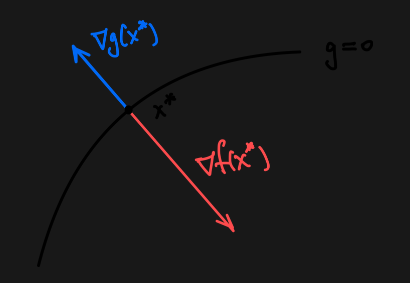
\includegraphics[width=0.4\textwidth]{Figs/kkt.png}
\caption{Graphical interpretation of KKT conditions on a single constraint.}
\label{fig:kkt}
\end{figure}


\subsection{Benefits of the Dual Problem}

The dual problem can be advantageous because it may be easier to solve than the primal problem. Additionally, it offers insights into the sensitivity of the optimal value to changes in the objective function or constraints. The duality gap, the difference between the solutions of the primal and dual problems, is zero under certain conditions, which provides a certificate of optimality for the primal solution.

%
%
%

\section{Smooth functions}
\subsection{Definition by derivatives}
\subsection{Definition by coefficients of Fourier transform}

\section{Singular value decomposition (SVD)}
\subsection{Definition}
\subsection{Properties}
\subsection{Applications}

%
%
%
%
%
%
%
%
%
%
%
%
%
%
%
%

\chapter{The Point Neuron}

\section{A Learning system}
\subsection{Supervised vs unsupervised learning vs reinforcement learning}

%
%
%

\subsection{Basic concepts in learning theory}

%
%
%

\subsection{The challenge of learning}
\subsubsection{Trainability}
The learning system's ability to arrive at the correct solution.

\subsubsection{Expressibility (capacity)}
The learning system's ability to represent complex functions.
We can choose the model for a given problem some examples are:
\begin{itemize}
    \item Linear regression $y = \mathbf{w}^T \mathbf{x} = b$
    \item Quadratic regression $y = \mathbf{w_2} \lVert \mathbf{x} \rVert^2 + \mathbf{w_1} \mathbf{x} + \mathbf{w_0}$
    \item Polynomial regression $y = \sum_{i=0}^{N} \mathbf{w_i} \lVert \mathbf{x} \rVert^i$
            While the equation is non linear in the input, it is quadratic in the weights, so the error function is convex.

    \item Fourier series $y = \sum_{k=n}^{N} \mathbf{w_k} e^{i k \pi \mathbf{x} / P}$ 
\end{itemize}
Using reacher models we can represent more complex functions, but we need to be careful with overfitting.

\subsubsection{Generalization}

\begin{definition}[Training error]
$E_{tr} = \frac{1}{P} \sum_{\mu=1}^{P} (\hat{y}(\mathbf{x}^\mu, \mathbf{w}) - y^\mu)^2$
\end{definition}

\begin{definition}[Generalization error]
$E_{g} = \int P(\mathbf{x}) (\hat{y}(\mathbf{x}, \mathbf{w}) - y(\mathbf{x}))^2 d\mathbf{x}$
\end{definition}

We have 2 assumptions:
\begin{itemize}
    \item All input come from some distribution $x^\mu \sim P(x)$. In most applications we will assume that any sample from the training set is an independent and identically distributed (i.i.d.) sample from the distribution $P(x)$.
    \item There is an underlying pattern in the labels $y^\mu \sim P(y|x^\mu)$
\end{itemize}
We will always have $E_{tr} \leq E_{g}$.

\begin{figure}
    \centering
    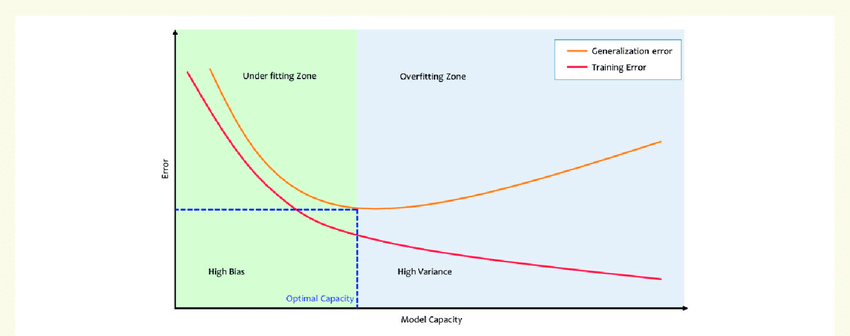
\includegraphics[width=\linewidth]{Figs/capacity-error-curve.png}
    \caption{Capacity VS Error curve}
    \label{fig:scenario1}
\end{figure}

\subsubsection{No free lunch theorem (NFT)}
\begin{theorem}
    If an algorithm performs well on a certain class of problems, it necessarily pays for that with degraded performance on the set of all remaining problems.
\end{theorem}
\begin{corollary}
    Every 2 optimization algorithms are equivalent when their performance is averaged across all possible problems.
\end{corollary}

\subsubsection{Regularization}
\begin{definition}
    Regularization is a technique used to prevent overfitting by discouraging overly complex models.
\end{definition}

\begin{itemize}
    \item Sparse parameters: $E_{tr}(\mathbf{w}) = \sum_{\mu=1}^{P} (\hat{y}(\mathbf{x}^\mu, \mathbf{w}) - y^\mu)^2 + \lambda \lVert \mathbf{w} \rVert_0$
    \item L1 regularization (Lasso): $E_{tr}(\mathbf{w}) = \sum_{\mu=1}^{P} (\hat{y}(\mathbf{x}^\mu, \mathbf{w}) - y^\mu)^2 + \lambda \lVert \mathbf{w} \rVert_1$
    \item L2 regularization: $E_{tr}(\mathbf{w}) = \sum_{\mu=1}^{P} (\hat{y}(\mathbf{x}^\mu, \mathbf{w}) - y^\mu)^2 + \lambda \lVert \mathbf{w} \rVert_2^2$
        We can solve this optimization problem analytically, and the solution is $\mathbf{w}^* = (\mathbf{X}\mathbf{X}^T + \lambda \mathbf{I})^{-1}\mathbf{X}\mathbf{Y}$
\end{itemize}


%
%
%

\section{Linear regression}
\subsection{Definition of the problem}
\begin{itemize}
    \item $\vec{x} \in \mathbb{R}^N$ - the input vector
    \item $y = \sum_{i=1}^{N} w_i x_i = \vec{w}^T \vec{x}$ - the output
    \item The training set: $\{(\vec{x}^1, y^1), (\vec{x}^2, y^2), \ldots, (\vec{x}^P, y^P)\} = \{(\vec{x}^\mu, y^\mu)\}_{\,\mu=1}^{P}$
    \item The training error of a single example (MSE): $\epsilon^\mu = (\hat{y}(\vec{x}^\mu, \vec{w}) - y^\mu)^2 = (\vec{w}^T \vec{x}^\mu - y^\mu)^2$
    \item The average error of a training set: $E_{tr}(\vec{w}) = \frac{1}{P} \sum_{\mu=1}^{P} \epsilon^\mu = \frac{1}{P} \sum_{\mu=1}^{P} (\vec{w}^T \vec{x}^\mu - y^\mu)^2$
    \item The generalization error: $E_{g}(\vec{w}) = \int P(\vec{x}) (\vec{w}^T \vec{x} - y(\vec{x}))^2 d\vec{x}$
\end{itemize}

%
%

\subsection{Points in general position}
\begin{definition}
A set of points in \(\mathbb{R}^n\) is said to be in \textit{general position} if no subset of \(m+1\) points lies in any \(m\)-dimensional hyperplane, for any \(m < n\). In simpler terms, in \(\mathbb{R}^2\) (the plane), points in general position means that no three points are collinear. Similarly, in \(\mathbb{R}^3\), no four points lie on the same plane. This concept extends to higher dimensions accordingly.
\end{definition}

%
%

\subsection{The optimal solution}

We will define the (empirical) feature covariance matrix of the input as:
\begin{align*}
    \mathbf{C_{tr}} = \frac{1}{P} \sum_{\mu=1}^{P} \vec{x}^\mu (\vec{x}^\mu)^T \\
    (\mathbf{C_{tr}})_{ij} = \frac{1}{P} \sum_{\mu=1}^{P} x_i^\mu x_j^\mu
\end{align*}

We will define the input-output covariance vector as:
\begin{align*}
    \vec{U_{tr}} = \frac{1}{P} \sum_{\mu=1}^{P} y^\mu \vec{x}^\mu \\
    (\vec{U_{tr}})_i = \frac{1}{P} \sum_{\mu=1}^{P} y^\mu x_i^\mu
\end{align*}

The weights that achieve the minimal loss must satisfy $\nabla E_{tr}(\vec{w}) = 0$. 
\begin{align*}
    \nabla \left(\frac{1}{P} \sum_{\mu=1}^{P} (\vec{w}^T \vec{x}^\mu - y^\mu)^2\right) = 0 \quad \\
    \Rightarrow \quad \frac{1}{P} \sum_{\mu=1}^{P} 2(\vec{w}^T \vec{x}^\mu - y^\mu) \vec{x}^\mu = 0 \\ 
    \Rightarrow \frac{1}{P} \sum_{\mu=1}^{P} (\vec{w}^T \vec{x}^\mu) \cdot \vec{x}^\mu  - \frac{1}{P} \sum_{\mu=1}^{P} y^\mu \vec{x}^\mu = 0 \\
    \Rightarrow \frac{1}{P} \sum_{\mu=1}^{P} \vec{x}^\mu (\vec{x}^\mu)^T \vec{w}  - \frac{1}{P} \sum_{\mu=1}^{P} y^\mu \vec{x}^\mu = 0 \\
    \Rightarrow \mathbf{C_{tr}} \vec{w} - \vec{U_{tr}} = 0 \\
\end{align*}

Alternatively, in vectorized notation:
\begin{align*}
    \mathbf{X} &= (\vec{\mathbf{x}}_1, \vec{\mathbf{x}}_2, \ldots, \vec{\mathbf{x}}_P) \in \mathbb{R}^{N \times P}, \quad
    \tilde{\mathbf{y}} = (y_1, y_2, \ldots, y_P) \in \mathbb{R}^P \\
    \nabla_{\mathbf{w}} E_{\text{tr}} (\mathbf{w}) &= 0 \\
    \frac{1}{P} \nabla_{\mathbf{w}} \lVert \mathbf{X}^T\mathbf{w} - \vec{\mathbf{y}} \rVert^2 &= 0 \\
    \nabla_{\mathbf{w}} (\mathbf{X}^T\mathbf{w} - \vec{\mathbf{y}})^T (\mathbf{X}^T\mathbf{w} - \vec{\mathbf{y}}) &= 0 \\
    \nabla_{\mathbf{w}} (\mathbf{w}^T\mathbf{X}\mathbf{X}^T\mathbf{w} + \vec{\mathbf{y}}^T\vec{\mathbf{y}} - 2\mathbf{w}^T\mathbf{X}\mathbf{Y}) &= 0 \\
    2\mathbf{X}\mathbf{X}^T\mathbf{w} - 2\mathbf{X}\mathbf{Y} &= 0 \\
\end{align*}

\subsubsection{The solution for P $\geq$ N}

\begin{theorem}
    The matrix \(\mathbf{C_{tr}}\) is positive definite if the input vectors are in general position and \(P \geq N\).
\end{theorem}

\begin{proof}
    \begin{align*}
        \mathbf{C_{tr}} &= \frac{1}{P} \sum_{\mu=1}^{P} \vec{x}^\mu (\vec{x}^\mu)^T \\
        \vec{v}^T \mathbf{C_{tr}} \vec{v} &= \frac{1}{P} \sum_{\mu=1}^{P} \vec{v}^T \vec{x}^\mu (\vec{x}^\mu)^T \vec{v} \\
        &= \frac{1}{P} \sum_{\mu=1}^{P} (\vec{v}^T \vec{x}^\mu) (\vec{v}^T \vec{x}^\mu)^T \\
        &= \frac{1}{P} \sum_{\mu=1}^{P} \lVert \vec{v}^T \vec{x}^\mu \rVert^2 \geq 0
    \end{align*}
\end{proof}

\begin{theorem}
    The optimal weights that minimize the training error are given by:
    \begin{align*}
        \mathbf{w}^* &= (\mathbf{X}\mathbf{X}^T)^{-1}\mathbf{X}\mathbf{Y} = \mathbf{C_{tr}}^{-1}\mathbf{U_{tr}}
    \end{align*}
\end{theorem}


%

\subsubsection{The solution for P $<$ N}

\textcolor{red}{TODO}

%
%

\subsection{Learning with noisy teacher}

\textcolor{red}{The teacher provides noisy labels to the training set. The noise is modeled as a Gaussian distribution with zero mean and variance $\sigma^2$. The training error is now given by:}

%
%
%


\section{The point neuron}
\subsection{The neuron model}
\begin{definition}[The neuron model]\ \\
    Let $\vec{x} \in \mathbb{R}^N$ - input vector (it can be real values, binary (logic) or represent spikes), \\
    $\vec{w} \in \mathbb{R}^N$ - weight vector (synaptic weights), \\  
    $b \in \mathbb{R}$ - bias, \\
    $\phi : \mathbb{R} \rightarrow \mathbb{R}$ - activation function. \\
    then the output of the neuron is given by:
    \begin{align}
        y = \phi(\vec{w}^T \vec{x} + b)
    \end{align}
\end{definition}

\begin{figure}[ht]
    \centering
    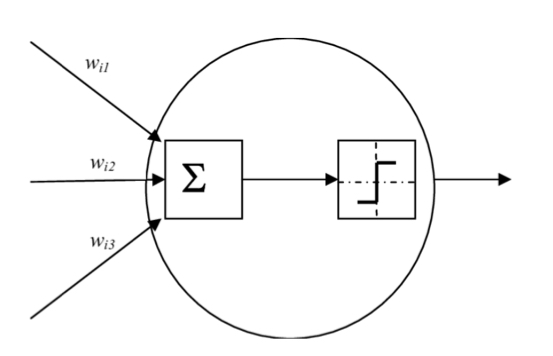
\includegraphics[width=0.3\textwidth]{Figs/point_neuron.jpeg}
    \caption{The neuron model}
    \label{fig:neuron_model}
\end{figure}


\subsection{Activation functions}
\subsubsection{Deterministic activation functions}
\begin{itemize}
    \item Linear activation function: $\phi(x) = \alpha x, \mathbb{R} \rightarrow \mathbb{R}$ (gives inear regression)
    \item Sigmoidal function - non-linear, bounded from below and above. e.g.,: 
    \begin{itemize}
        \item The sigmoid function (logistic) : $\phi(x) = \frac{1}{1 + e^{-x}}, \mathbb{R} \rightarrow (0, 1)$
        \item The hyperbolic tangent function: $\phi(x) = \tanh(x) , \mathbb{R} \rightarrow (-1, 1)$     
    \end{itemize}
    \item Threshold function: 
    \begin{itemize}
        \item Binary (heaviside) function: $\phi(x) = \begin{cases} 1, & \text{if } x \geq 0 \\ 0, & \text{if } x < 0 \end{cases}$ or $\phi(x) = sign(x) , \mathbb{R} \rightarrow \{-1, 1\}$
        \item The rectified linear unit (ReLU): $\phi(x) = \max(0, x) , \mathbb{R} \rightarrow [0, \infty)$ 
            The ReLY can be thought of the firing rate of a neuron (which can not be negative).
        \item The leaky ReLU: $\phi(x) = \max(\alpha x, x), \alpha \in (0, 1), \mathbb{R} \rightarrow (-\infty, \infty)$
    \end{itemize}
\end{itemize}

\begin{figure}
    \centering
    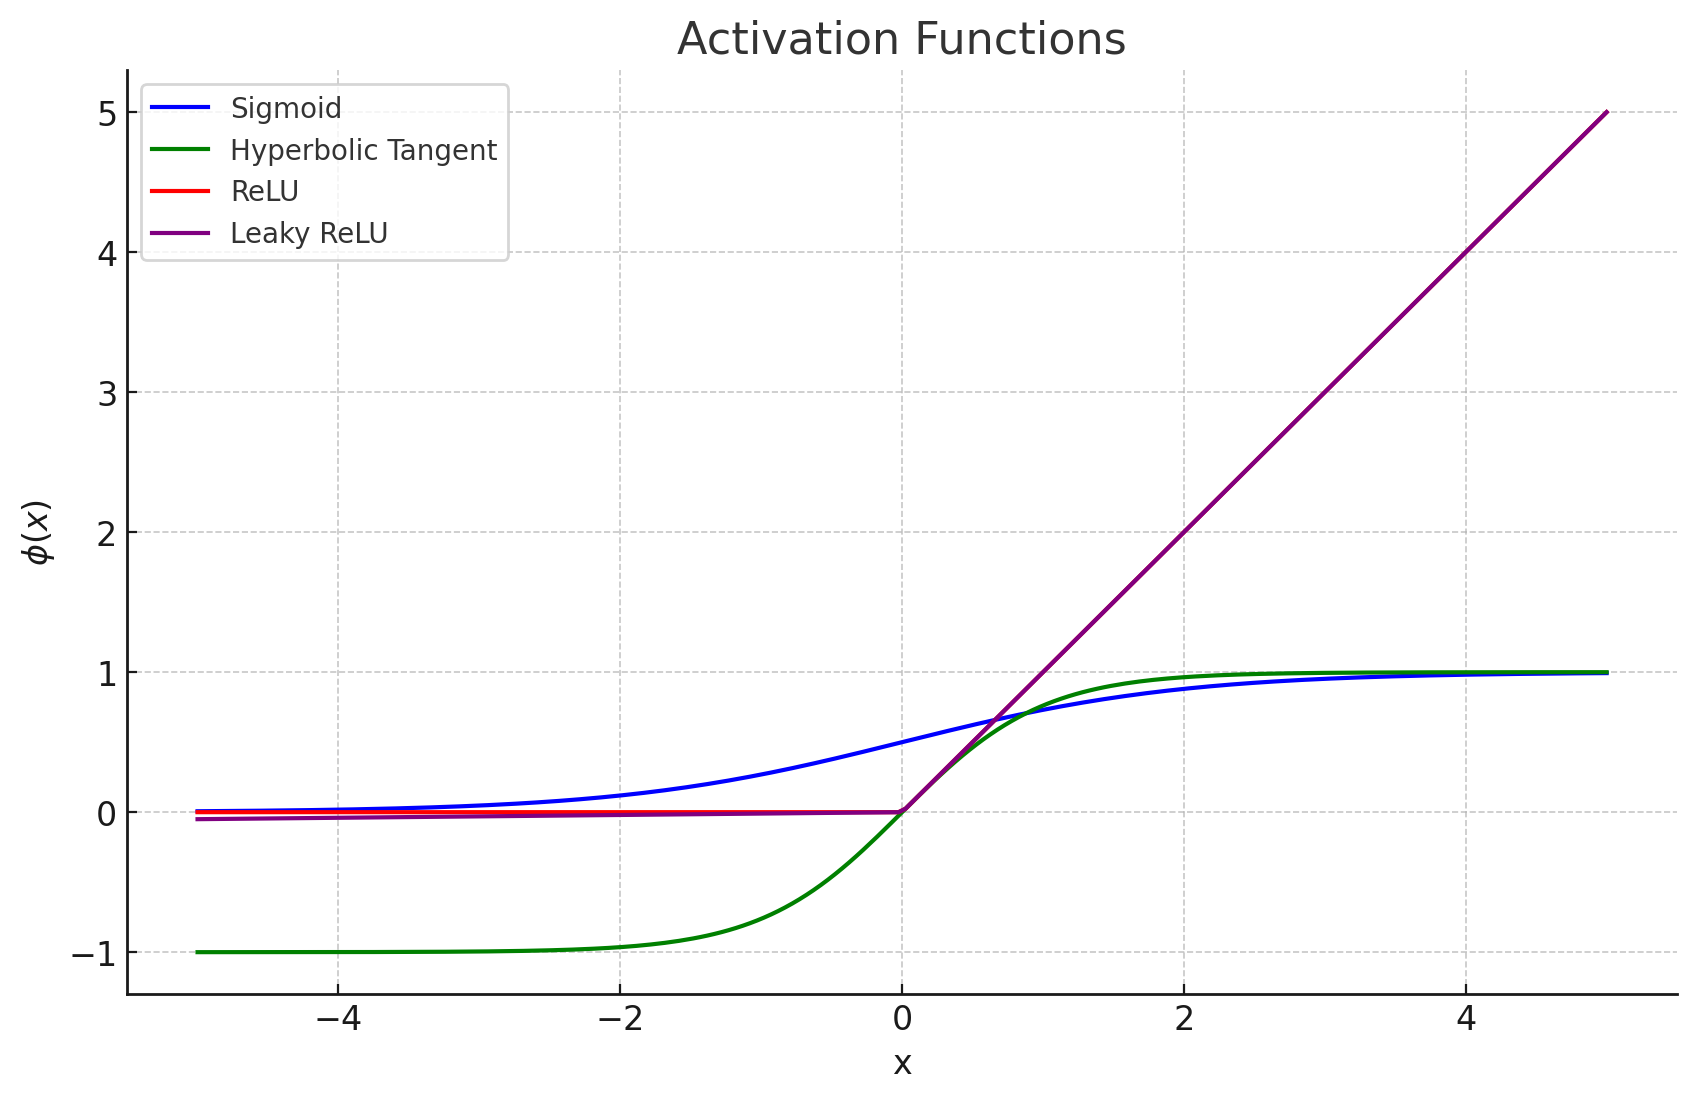
\includegraphics[width=0.6\linewidth]{Figs/activation_functions.png}
    \caption{Activation functions}
\label{fig:activation_functions}
\end{figure}

\subsubsection{Stochastic activation functions}
Demonstrate neuron that fire with some probability.
For example, The stochastic binary neuron: $\phi(x) = \begin{cases} 1 & \text{with probability } \frac{1}{1 + e^{-ax}} \\ 0 & \text{with probability } o.w \end{cases}$
    
\subsubsection{A spiking neuron}
Spiking neurons are more biological models of neurons which output a sequence of spikes over time, known as a spike train. The spike train can be mathematically described as follows:
\[
y(t) = \sum_k \delta(t_k - t),
\]
where \( y(t) \) is the output spike train at time \( t \), \( \delta \) represents the Dirac delta function, and \( t_k \) are the spike times. This formula sums up impulses at each spike time, creating a spike train.

The variables in the equation are characterized as:
\begin{itemize}
    \item \( \delta(t_k - t) \): Dirac delta function, which is 0 everywhere except at \( t = t_k \), where it is infinitely high with an integral of 1 over the entire real line, representing a spike at time \( t_k \).
    \item \( t_k \): The specific times at which the neuron fires a spike.
\end{itemize}

The output of the neuron can be considered through different models:
\begin{itemize}
    \item Inhomogeneous Poisson: The spikes are generated from a Poisson process with a rate parameter \( \lambda = ah \), meaning that the probability of a spike occurring in an infinitesimally small time window \( dt \) is \( \lambda dt = ahd\). Here, \( \lambda \) is not constant but may vary with \( h \), the input to the neuron.
    \item Integrate and fire: This model captures the behavior of a neuron that fires when its membrane potential crosses a specific threshold.
    \item HH neurons: Referring to the Hodgkin-Huxley model, will not be covered.
\end{itemize}


%
% 

\subsection{The binary perceptron}

\begin{definition}[The binary perceptron]
    The binary perceptron is a neuron model with a binary threshold activation function. The output of the binary perceptron is given by:
    \begin{align}
        \hat{y}(x|w,b) = sign(\vec{w}^T \vec{x} + b) \in \{-1, 1\}
    \end{align}
\end{definition}
For a given set of inputs $\{\vec{x}^\mu, y^\mu\}_{\mu=1}^{P}$, we want to find $w^*$ and $b^*$ that will hold 
\begin{align}
    \hat{y}(\vec{x}^\mu|w^*,b^*) = y^\mu, \quad \forall \mu
\end{align}
From a geometrical point of view, the binary perceptron is a linear classifier that separates the input space into two regions. 
The decision boundary is a hyperplane defined by $\vec{w}^T \vec{x} + b = 0$.
We ant all the projections of $\vec{x}^\mu$ on the hyperplane to be positive for $y^\mu = 1$ and negative for $y^\mu = -1$.

\begin{figure}
    \begin{subfigure}{0.5\textwidth}
        \centering
        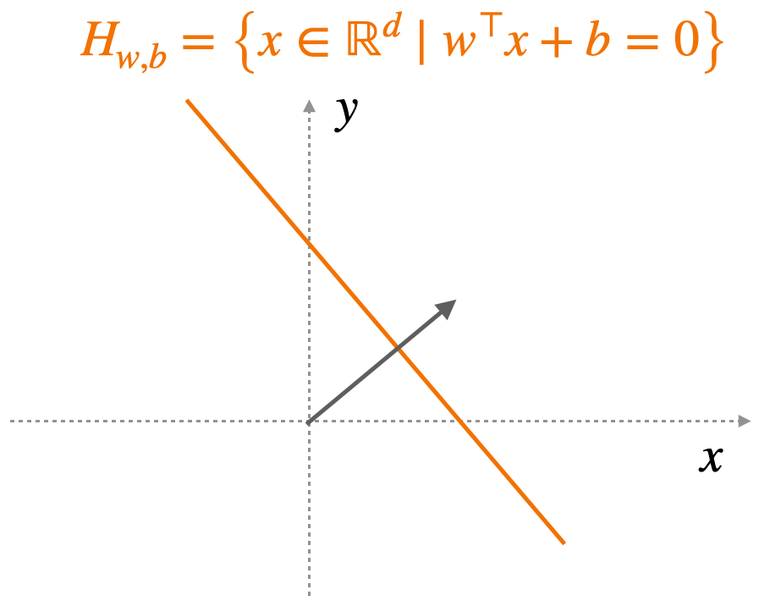
\includegraphics[width=\linewidth]{Figs/binary_hyperplane.png}
        \caption{The separation hyperplane of the binary perceptron}
    \label{fig:binary_perceptron}
    \end{subfigure}
    \begin{subfigure}{0.5\textwidth}
        \centering
        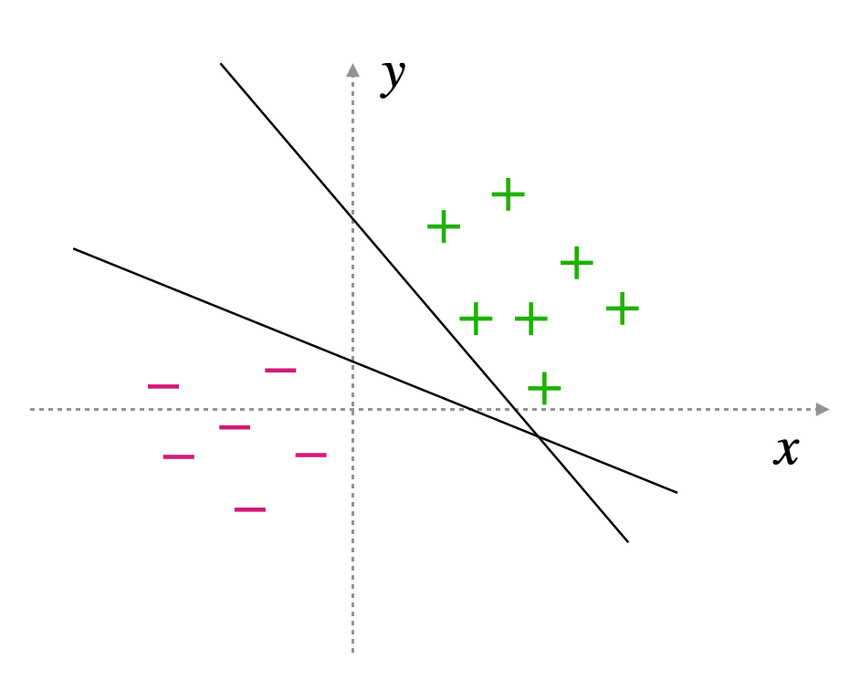
\includegraphics[width=\linewidth]{Figs/perceptron_2d.png}
        \caption{The binary perceptron in 2D}
    \label{fig:binary_perceptron2}
    \end{subfigure}
\end{figure}

We can simplify the problem by setting $b = 0$ and adding a constant input $x_0 = 1$ to the input vector $\vec{x}$, and now $w_0 = b$.
This simple perceptron makes a linear separation of the input space, and it can solve only linearly separable problems - 
For example, the XOR problem can not be solved by a single perceptron.


\subsection{The perceptron learning algorithm}
For a given set of inputs $\{\vec{x}^\mu, y^\mu\}_{\mu=1}^{P}$, we assume that the data is linearly separable.

\begin{algorithm}[H]
    \SetAlgoLined
    \caption{The Perceptron Learning Algorithm}
    
    \KwIn{Training set $D = \{(\vec{x}^t, y^t)\}$, learning rate $\eta$}
    \KwOut{Weight vector $\vec{w}$}
    
    Initialize weight vector $\vec{w}^1$ arbitrarily\;
    $t \leftarrow 1$\;
    
    \While{not converged}{
        Choose a random example $(\vec{x}^t, y^t)$ from $D$\;
        \If{$y^t \neq \text{sign}((\vec{w}^t)^T \vec{x}^t)$}{
            $\vec{w}^{t+1} \leftarrow \vec{w}^t + \eta y^t \vec{x}^t$\;
        }
        $t \leftarrow t + 1$\;
    }
\end{algorithm}


\begin{corollary}[Update rule of the weights]
    \begin{align}
        \bigtriangleup \vec{w}^t = \eta y^t \vec{x}^t \Theta (-y^t (\vec{w}^{t-1})^T \vec{x}^t)
    \end{align}
where $\Theta$ is the Heaviside step function defined as:
\[
    \Theta(x) = \begin{cases} 1, & \text{if } x > 0 \\ 0, & \text{if } x \leq 0 \end{cases}
\]
\end{corollary}

\begin{corollary}[Hebbian learning rule]
The perceptron learning algorithm is a form of Hebbian learning, where the weights are updated based on the correlation between the input and the output.
If the pre and the post synaptic neurons fire together, then the synapse between them is strengthened.
\[
    \bigtriangleup \vec{w}^t = \eta \frac{1}{2} (1 - y^t (\vec{w}^{t-1})^T \vec{x}^t) y^t \vec{x}^t = \frac{\eta}{2} (y^t -\hat{y}^t) \vec{x}^t = - \eta \epsilon^t \vec{x}^t
\]
where $\epsilon^t = \frac{1}{2} (y^t -\hat{y}^t)$ is the error of the perceptron (the error is signed) and because $y^t \in \{-1, 1\}$, the error is 0 if the perceptron is correct 
and otherwise it is equal to the sign of the correct label.
\end{corollary}


\begin{figure}
    \centering
    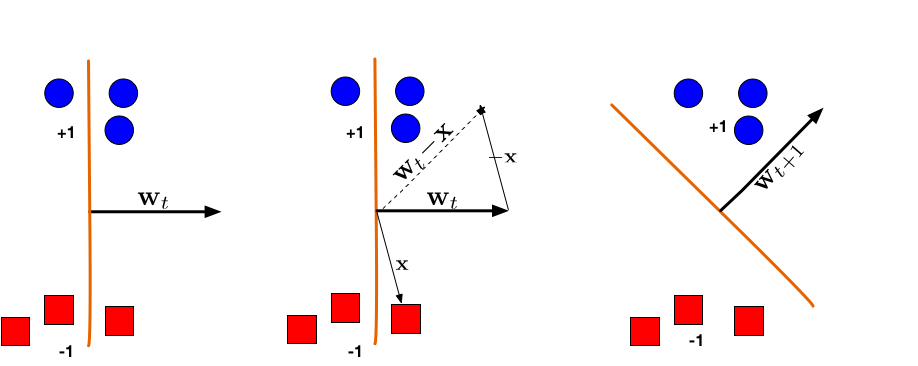
\includegraphics[width=\textwidth]{Figs/PerceptronUpdate.png}
    \caption{Illustration of a Perceptron update. \\ 
    (Left:) The hyperplane defined by $w_t$ misclassifies one red (-1) and one blue (+1) point. \\
    (Middle:) The red point x is chosen and used for an update. Because its label is -1 we need to subtract x from $w_t$. \\
    (Right:) The udpated hyperplane $w_{t+1}=w_t-x$ separates the two classes and the Perceptron algorithm has converged.}
    \label{fig:perceptron_learning}
\end{figure}


%
% 

\subsection{Cover's theorem (no proof)}
We have seen that simple perceptron can lean to perfoem linear binary separation given a set of P samples. 
But how large can P be? Intuitively, this maximum number of samples should depend on the dimensionality of the input space N.

\begin{definition}[Dichotomy]\ \\
    A dichotomy of a set of points is a partition of the set into two subsets.
\end{definition}

\begin{theorem}[Cover's theorem]
    Let $\{x^1, x^2, \ldots, x^P\}$ be a set of P points in $\mathbb{R}^N$ in general position. 
    The number of dichotomies that can be performed using a hyperplane that goes through the origin is given by:
    \begin{align}
        C(P,N) = 2 \sum_{k=0}^{N-1} \binom{P-1}{k}
    \end{align}
\end{theorem}

\begin{corollary}[The consequences of Cover's theorem]
    The number of dichotomies grows exponentially with the number of samples P, increasing much faster than but the number of linearly separable dichotomies.
    Exmaples: 
    \begin{itemize}    
        \item For P $\leq$ N, the number of dichotomies is $C(P,N) = 2^P$
        \item for P = 2N, the number of dichotomies is $C(2N,N) = \frac{1}{2} 2^{P}$
        \item For P $\gg$ N, the number of dichotomies is $C(P,N) \approx P^N$
    \end{itemize}
\end{corollary}
    
    

%
%
%


\section{SVM}
\subsection{The margin}

\begin{definition}[The margin of a point]\ \\
    The margin of a point $\vec{x}^\mu$ is the normalized distance from the point to the separating hyperplane:
    \begin{align}
        \delta^\mu(\vec{w}) = \frac{1}{|w|} y^\mu \vec{w}^T \vec{x}^\mu
    \end{align}
\end{definition}

\begin{definition}[The margin of the perceptron]\ \\
    The margin of the perceptron is the minimum margin of all the points:
    \begin{align}
        \delta(\vec{w}) = \min_{\mu} \delta^\mu(\vec{w}) = \frac{1}{|w|} \min_{\mu} y^\mu \vec{w}^T \vec{x}^\mu
    \end{align}
\end{definition}
We can see that our perceptron learning algorithm updates the weights if the margin is negative (that is, if the point is misclassified), 
and that every update increases the norm of the weights, so to normalize the margin we need to normalize the weights. \\
We can think of a the case where we want each point to have a margin ball of at least $\kappa$ and in that case the update rule will be:

\begin{align}
    \bigtriangleup \vec{w}^t = \eta \Theta(\kappa - \frac{ y^t \vec{w}^T \vec{x}^t}{|w|}) y^t \vec{x}^t = \eta \Theta(\kappa - \delta^t(w)) y^t \vec{x}^t
\end{align}

Our optimal solution $w^*$ will be the one that maximizes the margin, i.e., 
\[ 
    w^* = \operatorname*{argmax}_{w} \delta(w) = \operatorname*{argmax}_{w} \frac{1}{|w|} \min_{\mu \in [P]} y^\mu \vec{w}^T \vec{x}^\mu 
\] 

\begin{theorem}[Uniqueness of the solution (Vapnik, 1998)]\ \\
    The solution of the SVM optimization problem is unique.
\end{theorem}

\begin{figure}
    \centering
    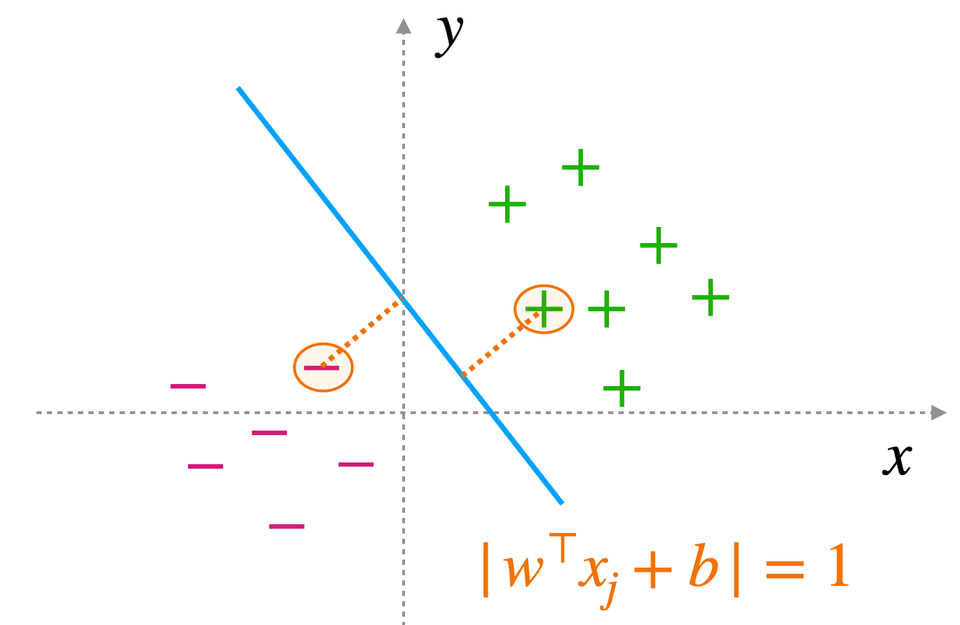
\includegraphics[width=0.6\textwidth]{Figs/svm.png}
    \caption{Max margin Linear classifier}
    \label{fig:margin}
\end{figure}

%
%

\subsection{The SVM optimization problem}

\subsubsection{The primal problem}

What we want to do is maximize the margin. However, as we have seen before, there is some duality between the margin and the norm of the weights.
Since on our measure of distance, we are normalizing by the norm, we can choose any norm that we would like. So we will choose it to be the inverse of the minimal margin
\begin{equation}
    \lVert w \rVert = \frac{1}{\delta}  
\end{equation}

Where \( \delta = \delta(w) = \min_{\mu} y^{\mu}w^T x^{\mu} \). So, for points on the minimal margin we have
\begin{equation}
    \delta = \frac{y^{\mu}w^T x^{\mu}}{\lVert w \rVert} = \delta y^{\mu}w^T x^{\mu}  
\end{equation}
or
\begin{equation}
    y^{\mu}w^T x^{\mu} = 1 
\end{equation}

Similarly, for points further from the hyperplane than the minimal distance, we have
\begin{equation}
    y^{\mu}w^T x^{\mu} =  \delta ^{\mu}  \lVert w \rVert = \frac{\delta^{\mu}}{\delta} \geq 1
\end{equation}

All together we can find conditions on our weights that
\begin{equation}
    y^{\mu}w^T x^{\mu} \geq 1 \quad \forall \mu.  
\end{equation}

What we want to do to maximize the minimal margin \( \delta \) is to minimize the norm of the weights \( w \). 
Since we have the freedom in choosing the norm of the weights, and we have chosen them to be \( 1/\delta \), this is equivalent to minimizing the norm of the weights with a fixed margin.

So, our optimization problem is to minimize the norm of the weights under the above conditions which we write as
\begin{equation}
    w^* = \arg \min_{\{w\}} \{ \lVert w \rVert \mid y^{\mu}w^T x^{\mu} \geq 1, \forall \mu \}. 
\end{equation}

or equivalently, our optimization problem is:
\begin{definition}[The primal problem of the SVM]
    \begin{align*}
        &\min_{\{w\}} \frac{1}{2} \lVert w \rVert^2 \\
        &\text{subject to} \quad  -y^{\mu}w^T x^{\mu} + 1 \leq 0, \forall \mu
    \end{align*}
\end{definition}




This is a constrained optimization problem, and we can solve it using the Lagrange multipliers method.

%
%

\subsubsection{The dual problem}
We now will consider b as a different variable (which is not in w) since it requires a different treatment.
The Lagrangian is given by:
\begin{equation}
    L(w, b, \alpha) = \frac{1}{2} \lVert w \rVert^2 - \sum_{\mu} \alpha^{\mu} (y^{\mu}(w^T x^{\mu} + b) - 1)
\end{equation}

Reminder - from the KKT conditions, we have that the optimal solution $w^*, b^*, \alpha^*$ holds:
\begin{itemize}
    \item Stationarity: 
    \begin{align*} 
        &\nabla_w L(w^*, b^*, \alpha^*) = 0 \Rightarrow \\
        &w_i^* - \sum_{\mu} (\alpha^*)^{\mu} y^{\mu} x_i^{\mu} = 0, \; i = 1, 2, \ldots, N \Rightarrow \\
        &w^* = \sum_{\mu} (\alpha^*)^{\mu} y^{\mu} x^{\mu} \\
        &\nabla_b L(w^*, b^*, \alpha^*) = 0 \Rightarrow \\
        &\sum_{\mu} (\alpha^*)^{\mu} y^{\mu} = 0
    \end{align*}
    \item Primal feasibility: \( -y^{\mu}((w^*)^T x^{\mu} + b) + 1 \leq 0, \; \forall \mu \)
    \item Dual feasibility: \((\alpha^*)^{\mu} \geq 0, \; \forall \mu \)
    \item Complementary slackness: \((\alpha^*)^{\mu} (-y^{\mu}((w^*)^T x^{\mu} + b) + 1) = 0, \; \forall \mu \)
\end{itemize}
We will construct a Lagrangian for the dual variables, $\alpha^\mu$. 
We begin with the second term in the Lagrangian, which yields:
\begin{equation}
    \sum_{\mu} \alpha^{\mu} \left[ -y^{\mu} \left( \sum_{i} w_i x_i^{\mu} + b \right) + 1 \right] = - \sum_{\mu} \alpha^{\mu} y^{\mu} \sum_{i} w_i x_i^{\mu} + \sum_{\mu} \alpha^{\mu} 
\end{equation}
(Note that the term due to $b$ dropped because of the constraint $\sum_{\mu} \alpha^{\mu} y^{\mu} = 0$.)

It is noted that the first term is simply $-\sum_{i} w_i^2$, which can be incorporated into the first term in the Lagrangian,
 $\frac{1}{2} \sum_{i} w_i^2 - \sum_{i} w_i^2 = -\frac{1}{2} \sum_{i} w_i^2$. This term can be rewritten as:
\begin{equation}
    -\frac{1}{2} \sum_{i} w_i^2 = -\frac{1}{2} \sum_{\mu,\nu} \alpha^{\mu} \alpha^{\nu} y^{\mu} y^{\nu} \sum_{i} (x_i^{\mu})^T x_i^{\nu} 
\end{equation}

Overall, we get the dual Lagrangian:
\begin{equation}
    g(\alpha) = \sum_{\mu} \alpha^{\mu} - \frac{1}{2} \sum_{\mu,\nu} \alpha^{\mu} \alpha^{\nu} y^{\mu} y^{\nu} \sum_{i} (x_i^{\mu})^T x_i^{\nu} 
\end{equation}

The optimum of this Lagrangian is found by maximizing with respect to \( \alpha \). Thus, we have the dual problem formulated as:
\begin{equation}
    \alpha^* = \arg \max_{\alpha} g(\alpha) 
\end{equation}

or equivalently:
\begin{definition}[The dual problem of the SVM]
    \begin{align*}
        &\max_{\alpha} \sum_{\mu} \alpha^{\mu} - \frac{1}{2} \sum_{\mu,\nu} \alpha^{\mu} \alpha^{\nu} y^{\mu} y^{\nu} \sum_{i} (x_i^{\mu})^T x_i^{\nu} \\
        &\text{subject to} \quad \alpha^{\mu} \geq 0, \quad \left( \sum_{\mu} \alpha^{\mu} y^{\mu} = 0 \right) \quad \forall \mu
    \end{align*}
\end{definition}

\subsubsection{The support vectors}
The support vectors are the points that lie on the margin, i.e., the points for which the margin is equal to 1.
The support vectors are the points that are closest to the hyperplane and are the most informative points for the classification.
The optimal solution of the SVM is a linear combination of the support vectors, and the other points do not affect the solution.
We can tell that by the KKT slackness condition, the points that are not support vectors have $\alpha^{\mu} = 0$.


%
%

\subsection{Dot product solution}

Using the dual problem of Support Vector Machines (SVM), we can characterize the solution using the support vector coefficients and the support vectors without even referencing the weights directly.

Recall that the weight vector \( w \) in the SVM formulation is given by a combination of the support vector coefficients and the support vectors themselves:
\begin{equation}
    w = \sum_{\mu} \alpha^{\mu} y^{\mu} x^{\mu} 
\end{equation}

With this, the SVM classifier can be written as a function of the input vector \( x \):
\begin{equation}
    \hat{y}(x) = \text{sign} \left( \sum_{\mu} \alpha^{\mu} y^{\mu} x^{\mu T} x \right) 
\end{equation}

Furthermore, for the learning process and the solution of the dual problem, it is essential to compute the \( P \times P \) matrix
\begin{equation}
    K_{\mu \nu} = x^{\mu} x^{\nu T} \quad (34)
\end{equation}

This matrix \( K \) is known as the kernel matrix, 
which encapsulates the inner products of all pairs of training examples in the feature space. 


%
%


\subsection{Soft-margin SVM}

Real data is rarely linearly separable, meaning that we will probably not have any weights such that $y^{\mu}w^T x^{\mu} > 0$ for all $\mu$.
Even if the data is linearly separable, we might want to allow some misclassification to avoid overfitting and to get a larger margin for better generalization.
We will relax the constraints of $y^{\mu}w^T x^{\mu} \geq 1$ for all $\mu$ by introducing the hinge loss function.

\begin{definition}[Hinge loss]
    The hinge loss is a loss function used in the soft-margin SVM that penalizes misclassification. It is defined as:
    \begin{align}
        \xi _{\mu} = \max(0, 1 - y^\mu \vec{w}^T \vec{x}^\mu)
    \end{align}   
\end{definition}

We can view $\xi _{\mu}$ as the measure of the inaccuracy we allow in classification: instead of requiring $y^{\mu}w^T x^{\mu} \geq 1$, 
we allow it to be at least 1 - $\xi _{\mu}$ with $\xi _{\mu} \geq 0$ for all $\mu$.
Thus, the optimization problem for the soft-margin SVM is:

\begin{definition}[The soft-margin SVM optimization problem]
    \begin{align*}
        \text{minimize} \quad E(\vec{w}, \vec{\xi}) = \frac{1}{P} \sum_{\mu=1}^P \xi _{\mu} + \lambda \lVert \vec{w} \rVert^2    \\
        s.t. \quad y^{\mu} \vec{w}^T \vec{x}^{\mu} \geq 1 - \xi _{\mu}, \quad \xi _{\mu} \geq 0, \quad \forall \mu
    \end{align*}
    Where $\lambda$ is the regularization parameter that balances the trade-off between the margin and the hinge loss.
    \begin{itemize}
        \item smaller $\lambda$ - prioritize correct classifications
        \item larger $\lambda$ - prioritize large margin
    \end{itemize}
\end{definition}


\subsubsection{The Dual Problem of Soft-margin SVM}

In soft-margin SVM, the primal optimization problem is defined as minimizing the empirical risk with an added regularization term that controls the margin's width, allowing for some misclassification as dictated by the slack variables $\vec{\xi}$. The primal problem is formulated as:

\begin{align*}
    \text{minimize} \quad E(\vec{w}, \vec{\xi}) &= \frac{1}{P} \sum_{\mu=1}^P \xi_{\mu} + \lambda \lVert \vec{w} \rVert^2 \\
    \text{s.t.} \quad y^{\mu} \vec{w}^T \vec{x}^{\mu} &\geq 1 - \xi_{\mu}, \quad \xi_{\mu} \geq 0, \quad \forall \mu
\end{align*}

To derive the dual problem, we introduce Lagrange multipliers $\alpha_{\mu}$ and $\beta_{\mu}$ for each of the constraints, leading to the Lagrangian:

\subsection{Derivation of the Dual Problem}

To derive the dual problem from the primal formulation of the soft-margin SVM, we start by constructing the Lagrangian that includes the primal objective function and the constraints weighted by Lagrange multipliers.

\begin{align*}
    \mathcal{L}(\vec{w}, \vec{\xi}, \vec{\alpha}, \vec{\beta}) &= \frac{1}{P} \sum_{\mu=1}^P \xi_{\mu} + \lambda \lVert \vec{w} \rVert^2 - \sum_{\mu=1}^P \alpha_{\mu} (y^{\mu} \vec{w}^T \vec{x}^{\mu} - 1 + \xi_{\mu}) - \sum_{\mu=1}^P \beta_{\mu} \xi_{\mu}
\end{align*}

The KKT conditions are used for the optimization problem where:

\begin{itemize}
    \item $\alpha_{\mu} \geq 0$ and $\beta_{\mu} \geq 0$ are the Lagrange multipliers associated with the inequality constraints.
    \item $\alpha_{\mu} (y^{\mu} \vec{w}^T \vec{x}^{\mu} - 1 + \xi_{\mu}) = 0$ is the complementary slackness condition, ensuring that for each $\mu$, either the constraint is active, and $\alpha_{\mu}$ is positive, or the constraint is inactive, and $\alpha_{\mu}$ is zero.
    \item $\beta_{\mu} \xi_{\mu} = 0$ ensures that if $\xi_{\mu} > 0$, then the corresponding $\beta_{\mu}$ is zero, and vice versa.
\end{itemize}

Taking the derivative of the Lagrangian with respect to $\vec{w}$ and setting it to zero gives us:

\begin{align*}
    \frac{\partial \mathcal{L}}{\partial \vec{w}} &= 2 \lambda \vec{w} - \sum_{\mu=1}^P \alpha_{\mu} y^{\mu} \vec{x}^{\mu} = 0 \\
    \Rightarrow \vec{w} &= \frac{1}{2\lambda} \sum_{\mu=1}^P \alpha_{\mu} y^{\mu} \vec{x}^{\mu}
\end{align*}

Similarly, taking the derivative with respect to $\xi_{\mu}$ and setting it to zero gives us:

\begin{align*}
    \frac{\partial \mathcal{L}}{\partial \xi_{\mu}} &= \frac{1}{P} - \alpha_{\mu} - \beta_{\mu} = 0 \\
    \Rightarrow \alpha_{\mu} + \beta_{\mu} &= \frac{1}{P}
\end{align*}

Substituting these into the Lagrangian, we eliminate $\vec{w}$ and $\vec{\xi}$ to obtain the dual function which we seek to maximize:

\begin{align*}
    \mathcal{L}(\vec{\alpha}) &= \frac{1}{P} \sum_{\mu=1}^P \xi_{\mu} + \lambda \lVert \vec{w} \rVert^2 - \sum_{\mu=1}^P \alpha_{\mu} (y^{\mu} \vec{w}^T \vec{x}^{\mu} - 1 + \xi_{\mu}) - \sum_{\mu=1}^P \beta_{\mu} \xi_{\mu} \\
    &= \lambda \vec{w}^T \vec{w} - w^T \sum_{\mu=1}^P \left( \alpha_{\mu} y^{\mu} \vec{x}^{\mu} \right) + \sum_{\mu=1}^P \alpha_{\mu} + \sum_{\mu=1}^P \left( \frac{1}{P}  - \alpha_\mu - \beta_{\mu} \right) \xi_{\mu} \\
    &= (\lambda - 2\lambda ) \vec{w}^T \vec{w} + \sum_{\mu=1}^P \alpha_{\mu} - \sum_{\mu=1}^P \left( 0 \right) \xi_{\mu} \\
    &= -\lambda \vec{w}^T \vec{w} + \sum_{\mu=1}^P \alpha_{\mu} \\
    &= \sum_{\mu=1}^P \alpha_{\mu} - \frac{1}{4\lambda} \sum_{\mu=1}^P \sum_{\nu=1}^P \alpha_{\mu} \alpha_{\nu} y^{\mu} y^{\nu} \vec{x}^{\mu T} \vec{x}^{\nu}
\end{align*}


The dual objective function to be maximized, with respect to the Lagrange multipliers $\vec{\alpha}$, is thus:

\begin{align*}
    \mathcal{L}(\vec{\alpha}) &= \sum_{\mu=1}^P \alpha_{\mu} - \frac{1}{4\lambda} \sum_{\mu=1}^P \sum_{\nu=1}^P \alpha_{\mu} \alpha_{\nu} y^{\mu} y^{\nu} \vec{x}^{\mu T} \vec{x}^{\nu} 
\end{align*}

The dual constraints, derived from the KKT conditions, must also be satisfied:

\begin{align*}
    0 \leq \alpha_{\mu} \leq \frac{1}{P} \quad \left( \text{and if we have b parameter} \quad \sum_{\mu=1}^P \alpha_{\mu} y^{\mu} = 0 \right)
\end{align*}

Combining these gives us the dual problem:

\begin{definition}[The dual problem of the soft-margin SVM]
    \begin{align*}
        \text{maximize} \quad \mathcal{L}(\vec{\alpha}) &= \sum_{\mu=1}^P \alpha_{\mu} - \frac{1}{4\lambda} \sum_{\mu=1}^P \sum_{\nu=1}^P \alpha_{\mu} \alpha_{\nu} y^{\mu} y^{\nu} \vec{x}^{\mu T} \vec{x}^{\nu} \\
        \text{subject to} \quad 0 &\leq \alpha_{\mu} \leq \frac{1}{P} \\
        \text{and} \quad &\sum_{\mu=1}^P \alpha_{\mu} y^{\mu} = 0
    \end{align*}
\end{definition}







%
%
%
%
%
%
%
%
%
%
%
%
%
%
%
%


\chapter{A Single Layer}

\section{The Kernel Method}

The kernel method is an essential tool in SVMs (Support Vector Machines), allowing for the creation of complex, nonlinear decision boundaries. The main advantage is that it facilitates the classification of data that is not linearly separable by transforming it into a higher-dimensional space where a linear separation becomes possible.

\subsection{The Dot Product Solution of the SVM}
The dual problem of SVM can be solved using only the support vector coefficients and the inner products of the samples in the feature space, bypassing the need to compute the weights directly. The weight vector $\vec{w}$ is given as a combination of the sample features weighted by the Lagrange multipliers.

\begin{align*}
    \vec{w} = \sum_{\mu=1}^P \alpha_{\mu} y_{\mu} \vec{x}_{\mu}
\end{align*}

\subsection{The XOR Problem}
The XOR function, which is not linearly separable, illustrates the limitations of linear classifiers. 
By transforming the input space to a higher dimension, we can find a hyperplane that separates the XOR classes linearly.
Consider the function $\Phi: \{0,1\}^2 \rightarrow \{0,1\}^3$ which is defined as follows:
\begin{equation*}
    \Phi(x_1, x_2) = \begin{bmatrix}
        x_1 \\
        x_2 \\
        x_1 x_2
    \end{bmatrix}
\end{equation*}
This mapping allows us to transform the input space into a new coordinate system where we can re-examine problems such as the logical gate with these new coordinates:
\begin{align*}
    (0, 0) &\mapsto (0, 0, 0) \\
    (1, 0) &\mapsto (1, 0, 0) \\
    (0, 1) &\mapsto (0, 1, 0) \\
    (1, 1) &\mapsto (1, 1, 1)
\end{align*}
And we can see that the XOR function is now linearly separable in this new space, for example by $w = [1, 1, -2]$.


\subsection{Nonlinear Decision Boundaries}
The kernel method enables the construction of nonlinear decision boundaries in the original feature space. 
This is achieved by transforming the input data to a higher-dimensional feature space where linear separation is possible.
Another example: elliptical decision boundaries can be created by transforming the 2D input space to a 3D space using the mapping \\
$\Phi(x_1, x_2) = (x_1^2, x_1 x_2, x_2^2)$.
The equation of the separating hyperplane in the new space is $w_1 x_1^2 + w_2 x_1 x_2 + w_3 x_2^2 + b = 0$ (we explicitly write the bias term $b$ here).

\begin{figure}[ht]
    \centering
    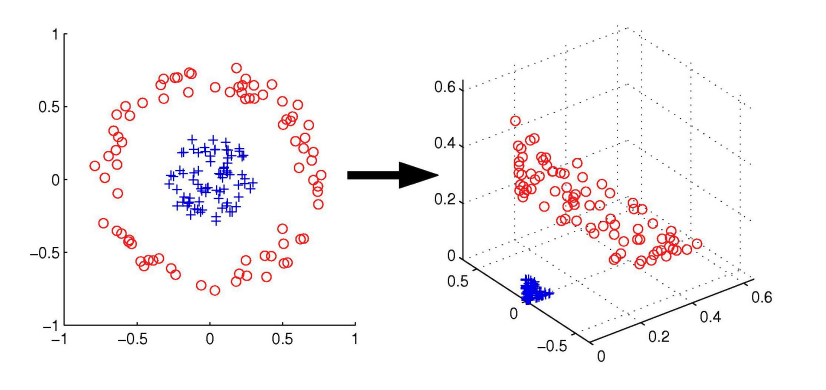
\includegraphics[width=0.7\textwidth]{./Figs/ellipse_kernel_trick.png}
    \caption{Transforming the input space to a higher dimension allows for the creation of nonlinear decision boundaries.}
    \label{fig:kernel_method}
\end{figure}


The expanded space $\vec{\phi}(\vec{x})$ is called the \textbf{feature space}.

There are two things at play here. First, Cover's function counting theorem. We have seen that the number of points that can be classified in an arbitrary manner depends on the dimensionality of the input. We are classifying $P$ points, but instead of in space $\vec{x} \in \mathbb{R}^N$ we use space $\vec{\phi} \in \mathbb{R}^M$ with $M \gg N$.

Second, we need the transformation to be \textbf{nonlinear}---we cannot just have linear relations embedded in higher dimensions (remember the general position requirements).

Potentially, we can choose a very large feature space with very complex transfer functions $\vec{\Phi}$. However, there are two major problems with that approach:

\begin{enumerate}
    \item \textbf{Generalization}. As we have discussed, with a large set of features and parameters, we are at risk of overfitting our data: in the feature space we have $M \ll N$ parameters.
    \item \textbf{Computation}. Working in high dimensions substantially increases computational costs.
\end{enumerate}

SVM offer solution to those two problems:

\begin{enumerate}
    \item \textbf{Generalization}. By looking for the optimal hyperplane, we are improving generalization. The optimal hyperplane has, at most, $P$ support vectors which will generally be significantly less than $M$ if we chose a very high-dimensional feature space.
    \item \textbf{Computation}. SVM uses the kernel method, which we will introduce shortly, which does not require the full feature space. Again it relies on the idea that the limiting factor here is the number of data points $P$ and not the size of the feature space $M$.
\end{enumerate}



\subsection{The Kernel Trick}

We assume that in the large feature space of \( M \) dimension, we choose the \( \vec{w} \) to be the optimal hyperplane. 
The classification from the feature space is given by
\begin{equation}
    \hat{y} = \text{sign}(\vec{w}^T \Phi(\vec{x})).
\end{equation}

From our derivations of the SVM algorithm, we know that the weights can be written in terms of the support vectors. In this case
\begin{equation}
    \vec{w} = \sum_{\mu=1}^{P} \alpha_{\mu} y^{\mu} \Phi(\vec{x}^{\mu}).
\end{equation}

If we plug this into our estimator, we get
\begin{equation}
    \hat{y} = \text{sign} \left( \sum_{\mu} \alpha_{\mu} y^{\mu} \Phi(\vec{x}^{\mu}) \Phi(\vec{x}) \right).
\end{equation}

We see that \( \Phi \) enters the classification only through an inner product with another \( \Phi \) at a different point. We therefore define
\begin{equation}
    K(x_1, x_2) = \Phi(x_1) \cdot \Phi(x_2)
\end{equation}

Remember that \( x_1, x_2 \in \mathbb{R}^N \) and \( \Phi(x_1), \Phi(x_2) \in \mathbb{R}^M \). The estimator is given by
\begin{equation}
    \hat{y} = \text{sign} \left( \sum_{\mu} \alpha_{\mu} y^{\mu} K(x_{\mu}, x) \right).
\end{equation}

The function \( K(x_1, x_2) \) is called the \textit{kernel function}. 
It is a transformation between two vectors of size \( N \) (\textbf{Not} \( M \)) to a scalar. \\
The large space of \( \Phi \) size \( M \) is not a problem here: if we know the form of the function \( K(\cdot, \cdot) \), 
then we don't need to do operations in the space of size \( M \).
The learning algorithm is solvable in the $\textbf{Dual Space}$, and only the kernel function is needed to solve the problem.

\subsection{Mercer's Theorem}
Mercer's theorem assures that a function can be used as a kernel if it corresponds to a dot product in some higher-dimensional space, 
given that it is symmetric and positive semidefinite. This theorem ensures the convergence of the SVM optimization problem.

\begin{theorem}[Mercer's Theorem]
    A symmetric function \( K(x, y) \) can be expressed as an inner product 
    \[
        K(x, y) = \Phi(x) \cdot \Phi(y)  
    \]
    for some feature space \( \Phi \) if and only if \( K(x, y) \) is positive semidefinite, i.e.,
    \[
        \int \int K(x, y) f(x) f(y) dx dy \geq 0 
    \]
    for every noramlizable function $f(x)$ in Hilbert space, i.e., $\int f^2(x) dx < \infty$, \\
    or equivalently, The Gram matrix $K$ 
    \[
    \begin{bmatrix}
        K(x_1, x_1) & K(x_1, x_2) & \cdots \\
        K(x_2, x_1) & \ddots & \\
        \vdots & & \ddots
    \end{bmatrix}
    \]
    is positive semi-definite (psd) for any collection \( \{x_1, \dots, x_n\} \).
\end{theorem}

\subsubsection{Qualitative proof}

The proof relied on extending the properties of symmetric functions in finite dimensions to kernels in infinite dimensions. 
Thus, in analogy to symmetric matrices, symmetric Kernels have a countable orthogonal basis of eigenvectors with real and positive eigenfunctions. 
In that case we can write:
\begin{equation}
    K(x, z) = \sum_{l} u_l(x)u_l(z)k_l
\end{equation}
Where \( k_l \) are real and are the spectra of \( K \) (analogous to the eigenvalue spectrum of symmetric matrices) 
If the kernel is positive semidefinite, then all \( k_l \geq 0 \) are positive, and we can take the square root of it and define 
\( \phi_l(x) = \sqrt{k_l}u_k(x) \) and the kernel is equal to
\begin{equation}
    K(x, z) = \sum_{l} \phi_l(x) \phi_l(z)
\end{equation}

The proof in the other direction is trivial: If \( K(x, z) \) can be written as a dot product then it is symmetric 
by definition and if the two functions are real then it is semidefinite by definition.


\subsection{Common Kernels}
Kernels can take various forms, each corresponding to a different type of feature space transformation.

\subsubsection{Exponential Kernel in 1D}
For 1D input $x, z \in \mathbb{R}$, the exponential kernel is defined as:
\begin{align*}
    K(x, z) = e^{xz}
\end{align*}
This kernel corresponds to an infinite-dimensional feature space transformation
\begin{align*}
    \Phi(x) = e^x = (1, x, \frac{x^2}{\sqrt{2!}}, \frac{x^3}{\sqrt{3!}}, \ldots)
\end{align*}
since
\begin{align*}
    K(x,z) = \phi(x) \cdot \phi(z) = \sum_{n=1}^{\infty} \frac{(xz)^n}{n!}
\end{align*}

\subsubsection{Admissible Kernels}
\begin {itemize}
    \item Sum of admissible kernels is an admissible kernel.
    \item Procuct of kernels (either element-wise or outer product) is an admissible kernel.
    \item Translation invariant kernels (stationary kernels) - a special class of kernels with the property that their 
    value depends only on the difference between the input vectors, not on the vectors themselves. For a translation invariant kernel \( K \), this implies that:
    \begin{equation}
        K(x, z) = K(x - z)
    \end{equation}
    
    Alternatively, this can be expressed as:
    
    \begin{equation}
        K(x, z) = K(\|x - z\|)
    \end{equation}
    
    where \( \| \cdot \| \) denotes some norm of the vector difference, often the Euclidean norm.
\end{itemize}

\subsubsection{Gaussian / Radial Basis Function (RBF) Kernel}
Is a translation invariant kernel, and is defined as:
\begin{align*}
    K(\vec{x}_\mu, \vec{x}_\nu) = \exp\left(-\frac{\|\vec{x}_\mu - \vec{x}_\nu\|^2}{2\sigma^2}\right) = \exp\left(-\gamma \|\vec{x}_\mu - \vec{x}_\nu\|^2\right)
\end{align*}
where \( \gamma = \frac{1}{2\sigma^2} \) is a hyperparameter that controls the kernel's width.

\begin{figure}[h]
    \centering
    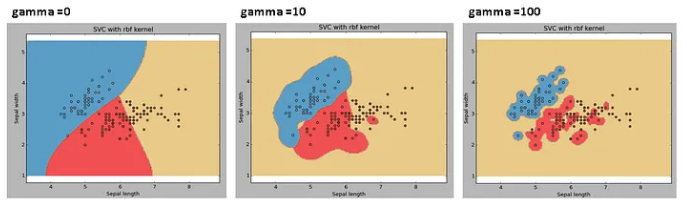
\includegraphics[width=0.7\textwidth]{./Figs/RBF_gamma.png}
    \caption{The effect of the hyperparameter \( \gamma \) on the RBF kernel.}
    \label{fig:RBF_kernel}
\end{figure}


\subsubsection{Polynomial Kernel}
The polynomial kernel is defined as follows:
\begin{align*}
    K(\vec{x}_\mu, \vec{x}_\nu) = (\vec{x}_\mu^T \vec{x}_\nu + c)^d
\end{align*}

\begin{figure}[h]
    \centering
    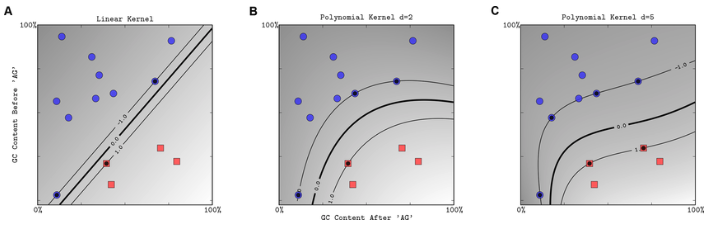
\includegraphics[width=0.7\textwidth]{./Figs/Poly_deg.png}
    \caption{The effect of the hyperparameter \( d \) on the polynomial kernel.}
    \label{fig:RBF_kernel}
\end{figure}

When the input data is transformed by this polynomial kernel, we effectively map our original \( N \)-dimensional data into a new feature space whose dimensionality corresponds to the number of monomials of degree up to \( d \) that can be formed from \( N + 1 \) elements, which includes the additional bias term represented by the constant \( 1 \) in the kernel function.

The dimensionality of the resulting feature space is given by the binomial coefficient, specifically:
\begin{equation}
    \text{dim}(\text{feature space}) = \binom{N + d}{d}
\end{equation}
This represents the number of unique ways to choose \( d \) items (with replacement) from a set of \( N + 1 \) items, which corresponds to the number of monomials of degree \( d \) or less that can be constructed from \( N + 1 \) features. This binomial coefficient is calculated as:
\begin{equation}
    \binom{N + d}{d} = \frac{(N + d)!}{d! \cdot (N + 1 - d)!}
\end{equation}
In the case of the polynomial kernel, this feature space is finite but can become very large as \( N \) or \( d \) increases, leading to a more expressive model that can capture complex relationships in the data.


\subsubsection{Sigmoid Kernel}
The sigmoid kernel is similar to the activation function used in neural networks:

\begin{align*}
    K(\vec{x}_\mu, \vec{x}_\nu) = \tanh(\gamma \vec{x}_\mu^T \vec{x}_\nu + r)
\end{align*}

\begin{figure}[ht]
    \centering
    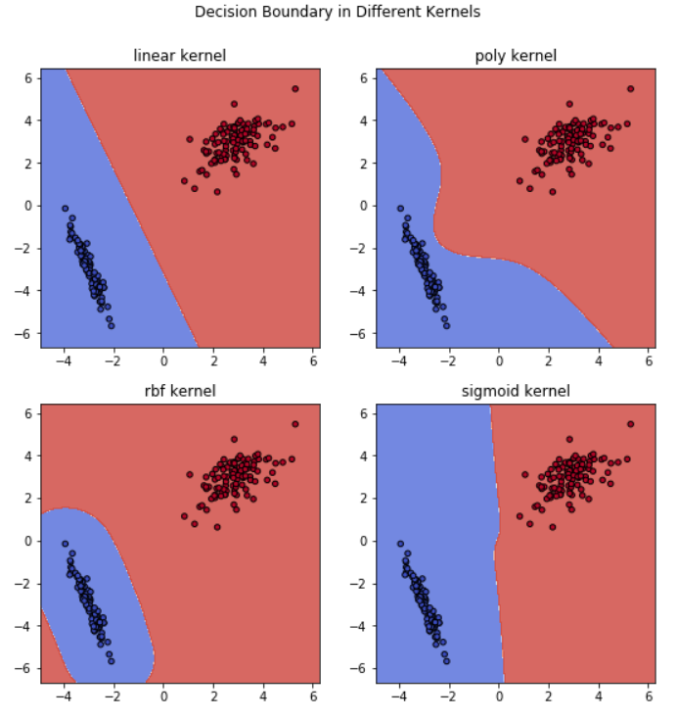
\includegraphics[width=0.7\textwidth]{./Figs/Kernels.png}
    \caption{Common kernel functions used in SVMs.}
    \label{fig:kernel_functions}
\end{figure}


The combination of the kernel method with slack variables in SVM leads to the creation of classifiers 
that have strong generalization performance for various classification tasks. 
This method allows the definition of complex decision surfaces without the high computational and generalization costs associated with large feature spaces.


\section{The Cerebellum}

\subsection{Cerebellar anatomy, physiology, and function}
The cerebellum accounts for approximately 10\% of the brain's volume but contains over 50\% of its neurons. It is known for its organized, preserved hierarchical feedforward structure. Traditionally associated with motor control and coordination, recent studies have linked the cerebellum to a variety of cognitive functions, including spatial reasoning, timing, language, and working memory.

\subsubsection{Basic facts}
The cerebellum is significant not only due to its volume but also due to the sheer number of neurons it contains. Its structure has been preserved across species, which indicates its importance in brain function.

\subsubsection{The cerebellum's function}
Historically, the cerebellum's function has been recognized as crucial for motor control. The classical view is that it fine-tunes motor control and coordination, interacting with the motor cortex and the motor system. The modern view extends its functions to interaction with various cortical areas, contributing to cognitive abilities.

\subsubsection{The cerebellum's anatomy}
The cerebellum's circuit includes parallel fibers, stellate and basket cells, Golgi cells, Purkinje cells, granule cells, climbing fibers, mossy fibers, and the Deep Cerebellar Nuclei. Each of these components plays a specific role in cerebellar processing.

\subsubsection{The cerebellar circuit}
Inputs to the cerebellum come through mossy fibers and a single climbing fiber, while the output is mediated by the Purkinje cells. An error signal is thought to be provided by the climbing fibers.

\begin{figure}[ht]
    \centering
    \begin{subfigure}[b]{0.5\textwidth}
        \centering
        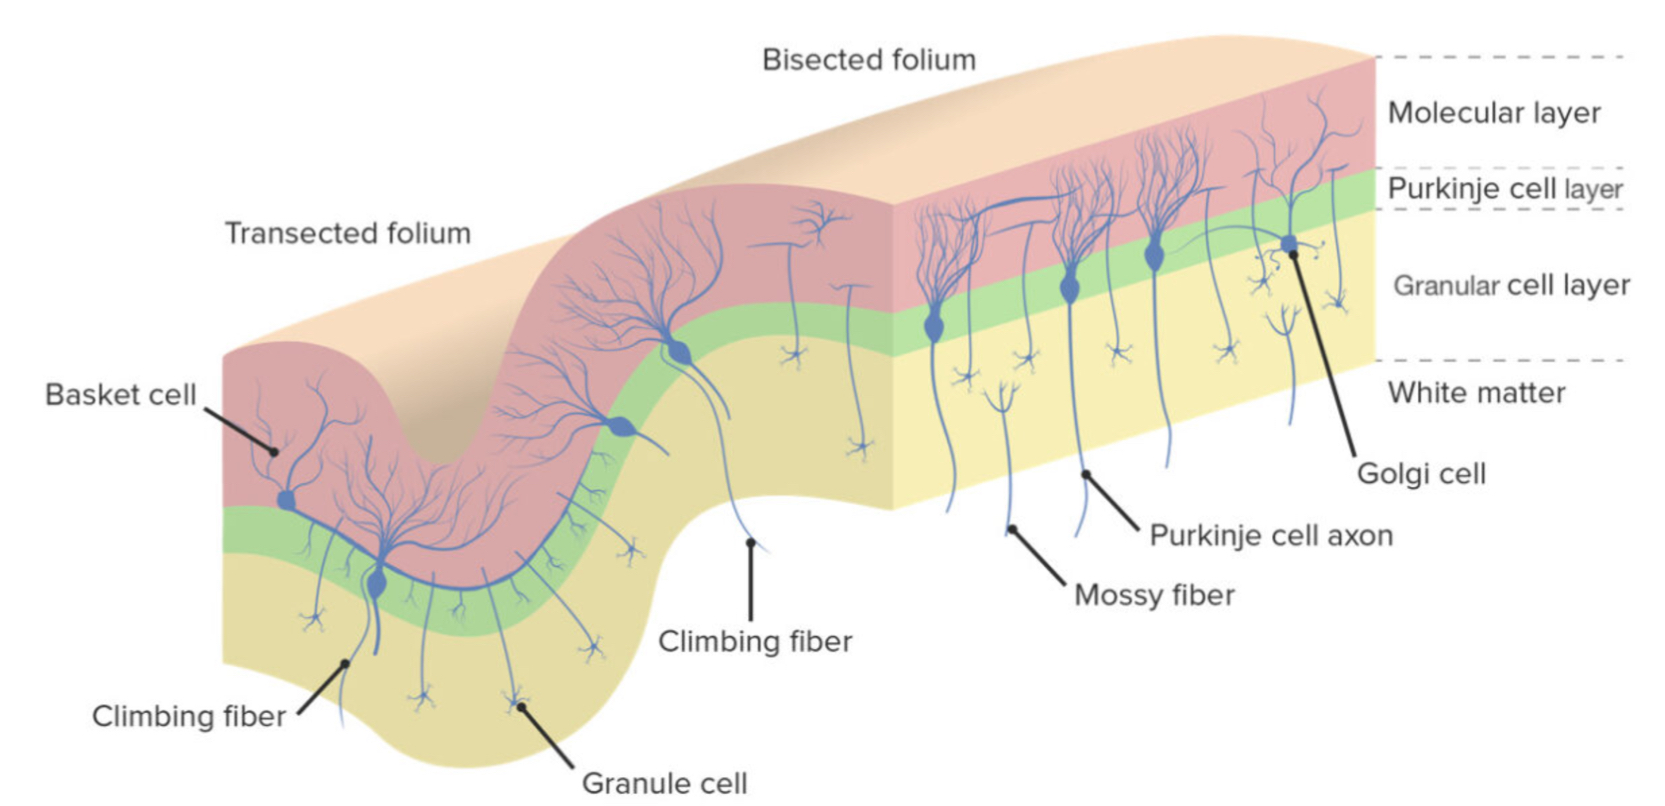
\includegraphics[width=\textwidth]{./Figs/cerebellums_anatomy.jpg}
        \label{fig:first_subfig}
    \end{subfigure}
    \hfill
    \begin{subfigure}[b]{0.5\textwidth}
        \centering
        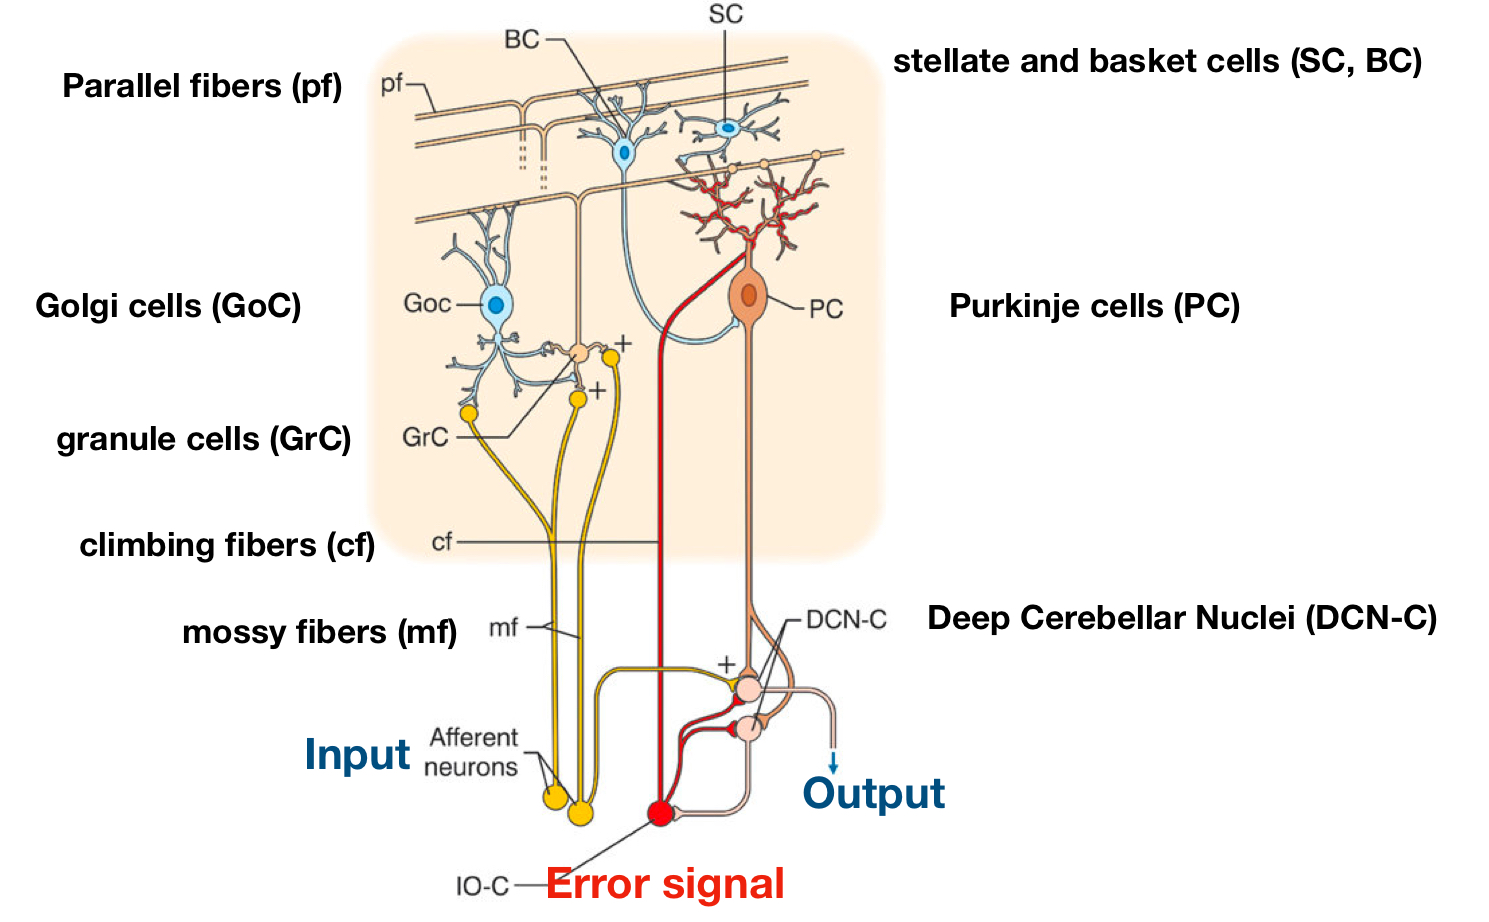
\includegraphics[width=\textwidth]{./Figs/cerebellums_anatomy2.jpeg}
        \label{fig:second_subfig}
    \end{subfigure}
    \hfill
    \begin{subfigure}[b]{0.5\textwidth}
        \centering
        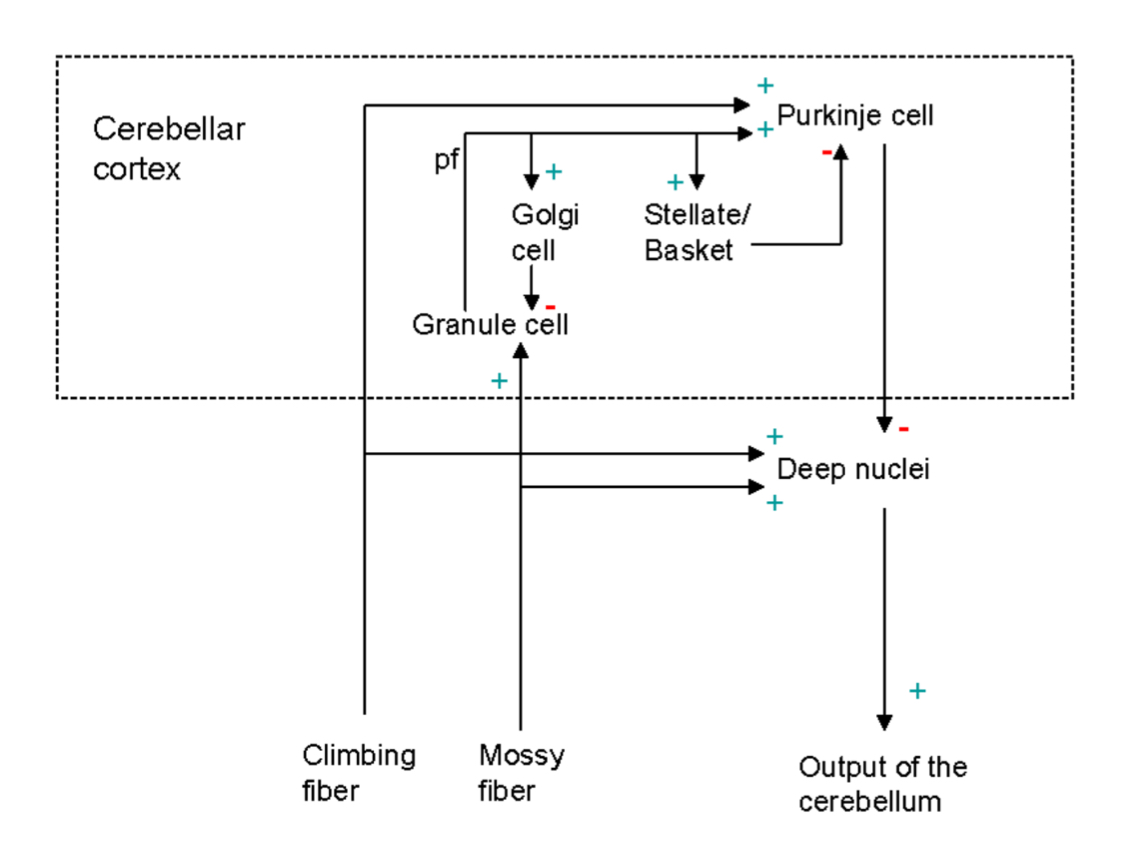
\includegraphics[width=\textwidth]{./Figs/cerebellums_anatomy3.jpeg}
        \label{fig:third_subfig}
    \end{subfigure}
    \label{fig:three_subfigures}
    \caption[short]{The cerebellum's anatomy.}
\end{figure}


\subsubsection{The cerebellar computational unit}
The computational unit of the cerebellum includes inputs from ~1,000 mossy fibers and a single climbing fiber, which are processed by ~200,000 parallel 
fibers and inhibitory interneurons, eventually influencing the output through a single Purkinje cell.

\subsubsection{Divergence and convergence in the cerebellum}
The cerebellum demonstrates a remarkable level of divergence and convergence. For instance, approximately 200 million mossy fibers diverge into 40 billion granule cells and then converge onto 15 million Purkinje cells. This massive divergence and convergence is crucial for the cerebellum's computational capacity.

\subsection{Plasticity and learning in the cerebellum}

\subsubsection{The Purkinje cell}
The Purkinje cell is unique for its planar dendritic arbor and is the sole output of the cerebellar cortex, inhibiting the Deep Cerebellar Nuclei. The plasticity observed in Purkinje cells is a central mechanism for cerebellar learning.
The Purkinje cell responds to climbing fiber inputs with a massive, all-or-none, 'complex spike'. The comlex spikes are relattively rare. 

\begin{figure}[ht]
\centering
\centering
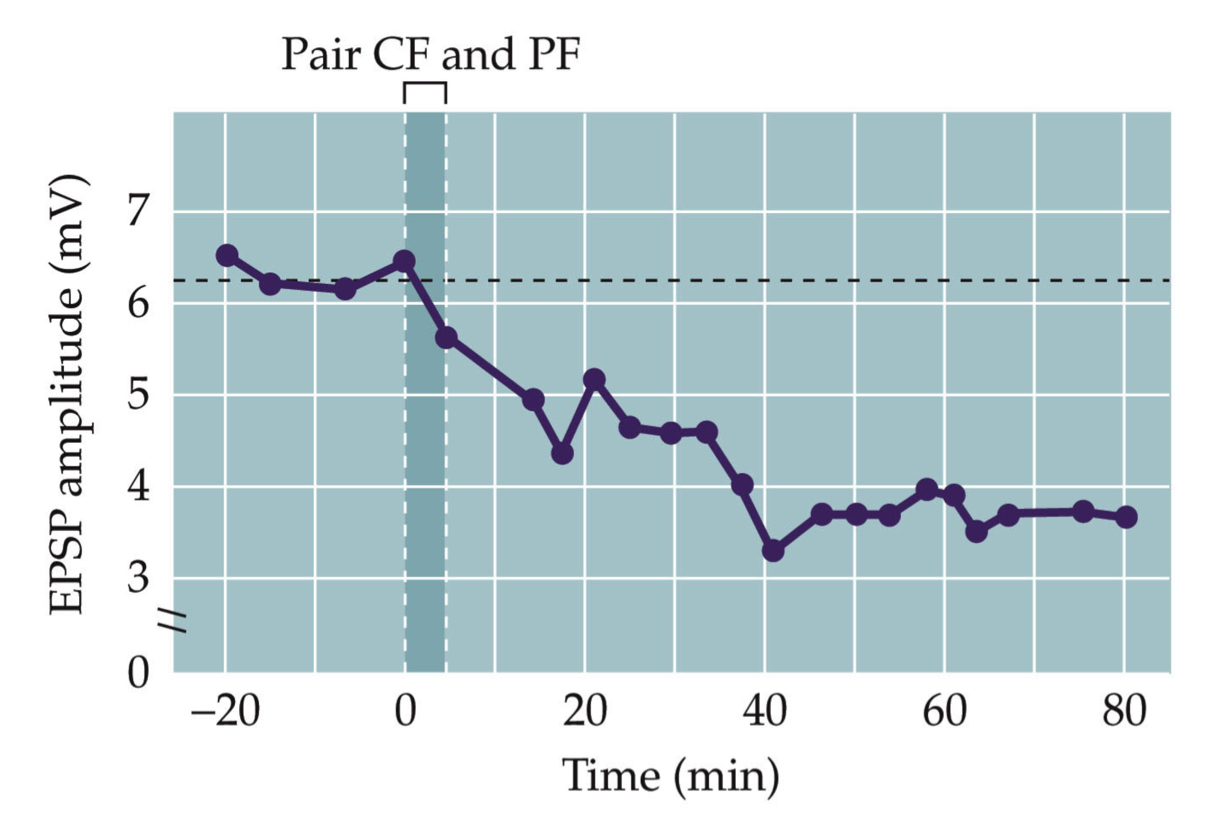
\includegraphics[width=0.6\textwidth]{./Figs/CF_PF.jpeg}
\label{fig:CF_PF}
\caption{When both CF (Climbing Fiber) and PF (Parallel Fiber) are active, LTD is induced.}
\end{figure}

\subsubsection{LTD and LTP in the Purkinje cell}
Long-Term Depression (LTD) and Long-Term Potentiation (LTP) in the Purkinje cells are responses to the synaptic activity between parallel fibers and climbing fibers. Climbing fibers signal errors, leading to LTD when paired with parallel fiber activation, and LTP occurs when parallel fibers are activated without climbing fibers.

\subsection{Marr-Albus theory for learning in the cerebellum}

\subsubsection{Motor learning in the cerebellum}
The Marr-Albus theory posits that the mossy fibers provide input patterns while the inferior olive generates an error signal when unexpected sensory input occurs. This framework helps explain how the cerebellum adapts and learns from motor errors, with the Purkinje cells playing a pivotal role.

\subsubsection{Main points the theory explains}
The theory explains the low frequency of complex spikes and climbing fiber firing, suggesting that these fibers do not contribute to ongoing motor execution but instead provide error signals for motor learning and adaptation.

\subsubsection{Extensions to the perceptron theory}
Recent studies have extended the perceptron theory, indicating that while the expansion of inputs helps, the benefits are limited without specific structural organization. Additionally, more layers in the cerebellar network model can lead to better learning outcomes.

%
%
%

\section{Gradient-based Learning}


%
%

\subsection{Batch learning}

\begin{definition}[Empirical Loss]\ \\
    The empirical loss is the average loss over the training set:
    \begin{align}
        E_{tr}(\vec{w}) = \langle \epsilon(\vec{w}, \vec{x}^\mu, y^\mu ) \rangle_\mu =\frac{1}{P} \sum_{\mu=1}^{P} \epsilon (\vec{w}, \vec{x}^\mu, y^\mu)
    \end{align}
\end{definition}

\textcolor{red}{TODO add figs}


Gradient-based learning is a continuous change in the weights in the direction of the negative gradient of the empirical loss.

\begin{algorithm}[H]
    \SetAlgoLined
    \caption{Batch Learning Gradient Descent}
    The change of the weights is in the direction of the negative gradient of the empirical loss:
    \[ \frac{d\vec{w}}{dt} = -\nabla_w E_{tr}(\vec{w}) \]
\end{algorithm}
    

\begin{claim*}[The GD update always reduces the loss]\ \\
    \begin{align}
        \frac{d E_{tr}(\vec{w})}{dt} = \frac{dE_{tr}(\vec{w})}{d\vec{w}}  \frac{d\vec{w}}{dt} = 
        \nabla_w E_{tr}(\vec{w}) \cdot -\nabla_w E_{tr}(\vec{w}) =  - \lVert \nabla_w E_{tr}(\vec{w}) \rVert^2 \leq 0
    \end{align}
\end{claim*}

The weaknesses of the simple batch learning are:
\begin{itemize}
    \item It guarantees to converge only a local minimum.
    \item It converges slowly in the vicinity of the minimum (since the gradient is small).
    \item It uses all the data to compute the gradient.
    \item Computing the gradient can be expensive.
\end{itemize}

\begin{definition}[Credit assignment problem]\ \\
    The credit assignment problem is the problem of distributing the 'blame' for the error among the weights.
\end{definition}


\subsection{Online learning}

Differently from batch learning, in incremental learning, the samples are presented one by one, and the weights are updated after each sample.

\begin{algorithm}[H]
    \SetAlgoLined
    \caption{Online Learning}
    Let $\{ (\vec{x}^t, y^t) \}$ be a sequence of samples, where $t$ is the time index of the sample that is given to the system. At each time step $t+1$ the system receives a new sample $(\vec{x}^{t}, y^{t})$ and updates the weights: 
    \[ \vec{w}^{t+1} = \vec{w}^{t} - \eta \nabla_w \epsilon(\vec{w}^{t}, \vec{x}^{t}, y^{t}) \]
    where $\eta$ is the learning rate.
\end{algorithm}


\begin{corollary}[The update rule of quadratic error]\ \\
    \begin{align*}
        \vec{w}^{t+1} &= \vec{w}^{t} - \eta \frac{1}{2} \nabla_w \lVert \hat{y}(\vec{x}^t, \vec{w}^t) - y^t \rVert^2  \\ 
        &= \vec{w}^{t} - \eta (\hat{y}(\vec{x}^t, \vec{w}^t) - y^t) \nabla_w \hat{y}(\vec{x}^t, \vec{w}^t) \\
        &= \vec{w}^{t} + \eta \delta^t \nabla_w \hat{y}(\vec{x}^t, \vec{w}^t)
    \end{align*}
    where $\delta^t = (y^t - \hat{y}(\vec{x}^t, \vec{w}^t))$ is $\neq 0$ if the perceptron is incorrect.
\end{corollary}

\begin{corollary}[The update rule of linear system]\ \\
    \begin{align}
        \vec{w}^{t+1} = \vec{w}^{t} + \eta \delta^t \vec{x}^t
    \end{align}
    

\end{corollary}


\subsection{Stochastic gradient descent (SGD)}
The learning rules on online learning minimize the training error, but what we actually want to minimize is the generalization error $E_{g}(\vec{w})$.
However, if we don't have the underlying distribution of the data point $\mathbb{P}(\vec{x})$ and of the labels $\mathbb{P}(y|\vec{x})$, we can't compute it.
In SDG, we try to improve the generalization error by adding some noise, stochasticity, to the learning process.

\begin{algorithm}[H]
    \SetAlgoLined
    \caption{Stochastic Gradient Descent (SGD)}
    Let $\{ (\vec{x}^t, y^t) \}$ be a sequence of samples, where $t$ is the time index of the sample that is given to the system.
    At each time step $t+1$ the system receives a new sample $(\vec{x}^{t}, y^{t})$ and updates the weights: 
    \begin{align*}
        \vec{w}^{t+1} = \vec{w}^{t} - \eta \nabla_w \epsilon(\vec{w}^{t}, \vec{x}^{t}, y^{t}) + \sigma \vec{\xi}(t) 
    \end{align*}
    where: 
    \begin{itemize}
        \item $\eta$ is the learning rate.
        \item $\sigma$ is the noise level.
        \item $\vec{\xi}(t)$ is a random vector of i.i.d. noise added to the dynamics.
    \end{itemize}
\end{algorithm}

The general idea is that:
\begin{align*}
    \langle \bigtriangleup \vec{w}^{t+1} \rangle = - \eta \langle \nabla_w \epsilon(\vec{w}^{t}, \vec{x}^{t}, y^{t}) \rangle \approx -\eta \nabla_w \epsilon_g (\vec{w}^{t}, \vec{x}, y) 
\end{align*}
For example, in order allow the deterministic system to overcome a local minimum, we need to push it beyond some error barrier.

%
%



%
%

\subsubsection{Analysis of online learning dynamics}


%
%

\subsubsection{Dynamics of learning in a linear network}


%
%

\subsubsection{Dynamics of the average}


%
%

\subsubsection{Controlling the variance (learning rate)}


%
%
%
%
%
%
%
%
%
%
%
%
%
%
%
%


\chapter{Deep Neural Networks}

\section{Multi-layered perceptrons vs the kernel method}
The differences between the kernel method and multi-layered perceptrons:
\begin{itemize}
    \item In MLP the is no expansion. We only relied on the non-linearity of the activation function.
    \item All the weights need to be learned to solve the problem. In the kernel method, we only need to learn the support vectors. 
    The feature space was used to untie the non-linearity of the problem.
    \item The benefits of the kernel method are:
    \begin{itemize}
        \item Better performance in high dimensional spaces.
        \item No need to engineer the features.
        \item In online learning (the kernel method used all the data to learn the support vectors).
        \item Complexity with very large data sets-like the ones required for many modern applications.
    \end{itemize}
\end{itemize}

\section{Structure}
\begin{itemize}
    \item The architecture consists of $L$ layers.
        Each layer $l$ has $N_l$ neurons, where $l = 1, 2, \ldots, L$.
        The first layer contains $N_0$ neurons, which is the dimensionality of the input.
        The $L-1$ hidden layers can contain any number of neurons.
        The last layer contains $N_L$ neurons, which is the dimensionality of the output and is determined by the problem.
        \begin{itemize}
            \item It can be any activation function for regression problems.
            \item For binary classification, the output can be binary.
            \item For multi-class classification, the output can be a softmax function, which has the following formula:
            $\hat{y_i} (s_i^L) = \frac{e^{s_i^L}}{\sum_{j=1}^{N_L} e^{s_j^L}} , \mathbb{R} \rightarrow (0, 1)$
            Here the readout neurons are no longer independent, and the output is normalized to sum to 1. 
            The outputs represent the probability of the input belonging to each class.
        \end{itemize}
    \item Denote by $\phi$ the non-linear activation function, by $W^l$ the matrix $N_l \times N_{l-1}$ of weights, that leads from $s^{l-1}$ to $s^l$. 
        The output of the $l$-th layer is given by 
        \begin{align*}
            s^l = \phi(W^l s^{l-1}) \\
            s_i^l = \phi(\sum_{j=1}^{N_{l-1}} W_{ij}^l s_j^{l-1}) = \phi((w_i^l)^T s^{l-1}) \\ 
            s^0 = x , N_0 = N, s^L = y
        \end{align*}
\end{itemize}

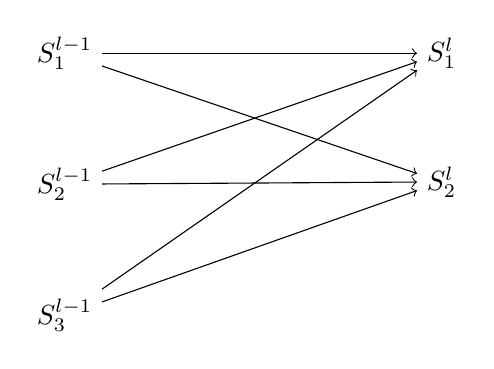
\begin{tikzpicture}[node distance=1cm and 2cm]
    % Define nodes
    \node (s1) {\( S_1^{l-1} \)};
    \node[below=of s1] (s2) {\( S_2^{l-1} \)};
    \node[below=of s2] (s3) {\( S_3^{l-1} \)};
    \node[right=of s1, xshift=2cm] (s4) {\( S_1^{l} \)};
    \node[below=of s4] (s5) {\( S_2^{l} \)};
    % Connect nodes
    \foreach \i in {1,...,3}
        \foreach \j in {4,...,5}
            \draw[->] (s\i) -- (s\j);
\end{tikzpicture}
\begin{tikzpicture}
    % Draw matrix
    \node[right=of s2, xshift=1cm] (matrix) {
        \( W^l = \begin{pmatrix}
            w_{11} & w_{12} & w_{13} \\
            w_{21} & w_{22} & w_{23}
        \end{pmatrix} \)
    };
    % Draw equation
    \node[right=of s5, xshift=2cm] (equation) {
        \( S^l = \phi(W^l S^{l-1}) \)
    };
\end{tikzpicture}

\subsection{Activation functions}
Same as the point neuron, the activation function can be any non-linear function.

\subsection{Loss functions}
The quadratic loss function is given by:
\begin{align*}
    \epsilon(\mathbf{w}) = \frac{1}{2} \lVert \hat{\mathbf{y}}(\mathbf{x}, \mathbf{w}) - \mathbf{y} \rVert^2
\end{align*}
Algorithms may include regularization terms to prevent overfitting, such as the L1 and L2 regularization terms, and the optimization is over Lagrangian.

%
%

\subsection{Credit assignment and backpropagation}

We have seen from gradient descent that: 
\begin{align*}
    \frac{d}{dt} w_{ij}^l = - \eta \frac{\partial \epsilon (w, x, y)}{\partial w_{ij}^l} = - \eta \delta^t \frac{\partial \hat{y}(w, x, y)}{\partial w_{ij}^l}
\end{align*}
Where $\delta^t = \hat{y}^t - y^t$ is the error of the network for the $t$-th sample.

By the chain rule (\ref{ssec:chain_rule}), we can write:
\begin{align*}
    \frac{dy(x,z)}{dw} = \frac{\partial y}{\partial x} \frac{dx}{dw} + \frac{\partial y}{\partial z} \frac{dz}{dw}
\end{align*}

\begin{figure}
    \centering
    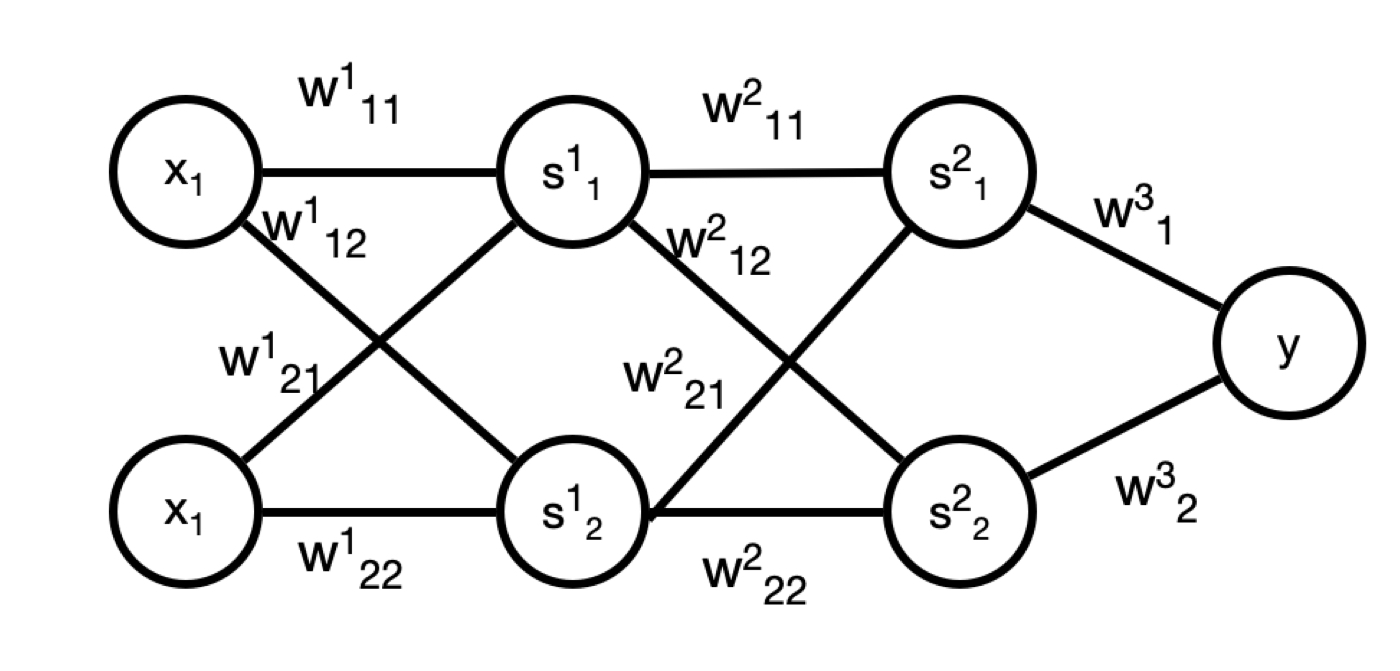
\includegraphics[width=0.8\textwidth]{Figs/backprop.jpeg}
    \caption{MLP with 2 hidden layers}
    \label{fig:backpropagation}
\end{figure}

We will now derive the backpropagation algorithm for a network with 2 hidden layers - 
the output of the network is given by $\hat{y} = \sigma(h^3)$, where $h^3 = w_1^3 s_1^2 + w_2^3 s_2^2$.

\begin{align*}
    \Delta w_{1}^{3} = -\eta \frac{\partial \epsilon (y|x^{\mu},y^{\mu})}{\partial w_{1}^{3}} = -\eta \delta^\mu \frac{\partial \hat{y}(w|x^{\mu})}{\partial w_{1}^{3}} = 
    -\eta \delta^\mu \sigma'(h^{3}(x^{\mu})) s_{1}^2(x^{\mu}) 
\end{align*}

\begin{align*}
    \Delta w_{11}^{2} = -\eta \frac{\partial \epsilon (y|x^{\mu},y^{\mu})}{\partial w_{2}^{11}} = -\eta \delta^\mu \frac{\partial \hat{y}(w|x^{\mu})}{\partial w_{11}^{2}} = \\
    -\eta \delta^\mu \frac{\partial \hat{y}(w|x^{\mu})}{\partial s_{1}^{2}} \frac{\partial s_{1}^{2}}{\partial w_{11}^{2}} = -\eta \delta^\mu \sigma'(h^{3}(x^{\mu})) w_{1}^{3} \sigma'(h_{1}^{2}) s_{1}^1
\end{align*}

\begin{align*}
    &\Delta w_{11}^{1} = -\eta \frac{\partial \epsilon (y|x^{\mu},y^{\mu})}{\partial w_{11}^{1}} = -\eta \delta^\mu \frac{\partial \hat{y}(w|x^{\mu})}{\partial w_{11}^{1}} = \\ 
    &-\eta \delta^\mu \frac{\partial \hat{y}(w|x^{\mu})}{\partial s_{1}^{2}} \frac{\partial s_{1}^{2}}{\partial w_{11}^{1}} = \\ 
    &-\eta \delta^\mu \sigma'(h^{3}(x^{\mu})) w_{1}^{3} \sigma'(h_{1}^{2}) w_{11}^{2} \sigma'(h_{1}^{1}) x_{1} 
    - \eta \delta^\mu \sigma'(h^{3}(x^{\mu})) w_{2}^{3} \sigma'(h_{2}^{2}) w_{12}^{2} \sigma'(h_{1}^{1}) x_{2} = \\
    &-\eta \delta^\mu \sigma'(h^{3}(x^{\mu})) \left[ w_{1}^{3} \sigma'(h_{1}^{2}) w_{11}^{2}  + w_{2}^{3} \sigma'(h_{2}^{2}) w_{12}^{2} \right] \sigma'(h_{1}^{1}) x_{1}
\end{align*}

We can simplify the notation by introducing matrix notation:
\begin{align*}
    &\Delta W^{3} = -\eta \delta^\mu \sigma'(h^{3}(x^{\mu})) S^{2} \\
    &\Delta W^{2} = -\eta \delta^\mu \sigma'(h^{3}(x^{\mu})) W^{3} \circ \sigma'(h^{2}(x^{\mu})) S^{1} \\
    &\Delta W^{1} = -\eta \delta^\mu \sigma'(h^{3}(x^{\mu})) W^{3} \circ \sigma'(h^{2}(x^{\mu})) W^{2} \circ \sigma'(h^{1}(x^{\mu})) X
\end{align*}
Note that the $\circ$ denotes the Hadamard product, which is the element-wise multiplication of two matrices.

In the same way, we can write the backpropagation algorithm for a network with $L$ hidden layers as follows:
\begin{equation}
    \frac{\partial \epsilon}{\partial W_{ij}^l} = \frac{\partial \epsilon}{\partial h_i^l} \frac{\partial h_i^l}{\partial W_{ij}^l} = 
    \frac{\partial \epsilon}{\partial h_i^l} s_j^{l-1}
\end{equation}
Where \( h_i^l = W^l \cdot s^{l-1} \) denotes the input to the \( i \)-th unit in the \( l \)-th layer, and \( s_i^l \) is the output thereof,
 \( s_i^l = \sigma (h_i^l) \). The derivative with respect to \( h_i^l \) can be further expanded:
\begin{equation}
    \frac{\partial \epsilon}{\partial h_i^l} = \sum_j \frac{\partial \epsilon}{\partial h_{j}^{l+1}} \frac{\partial h_{j}^{l+1}}{\partial h_i^l} = 
    \sum_j \frac{\partial \epsilon}{\partial h_{j}^{l+1}} W_{ji}^{l+1} \sigma'(h_i^l) 
\end{equation}
and for \( l = L \) we can compute \( \frac{\partial \epsilon}{\partial h_{i}^L} \) directly:
\begin{equation}
    \frac{\partial \epsilon}{\partial h_{i}^L} = \frac{\partial}{\partial h_{i}^L} \frac{1}{2} \sum_j (s_j^L - y_j)^2 = (s_i^L - y_i) \sigma'(h_i^L) 
\end{equation}


%
%
%

\section{Backpropagation derived using Lagrange multipliers}


%
%
%

\section{Dynamics of learning in a linear network (no proof)}

\begin{enumerate}
    \item Even for a linear network, the dynamics of learning is nonlinear, because of the minimization of the nonlinear loss function.
    \item The learning dynamics is controlled by the statistics of the data set used for training. The statistics is defined by input correlations and input-output correlations.
    \item In linear networks, the singular components of the data statistics are learned one after the other, where modes with higher singular values are learned first.
    \item These ideas can be extended to deeper networks.
    \item It gives an intuition to what's going on in nonlinear networks.
\end{enumerate}

\begin{figure}
    \centering
    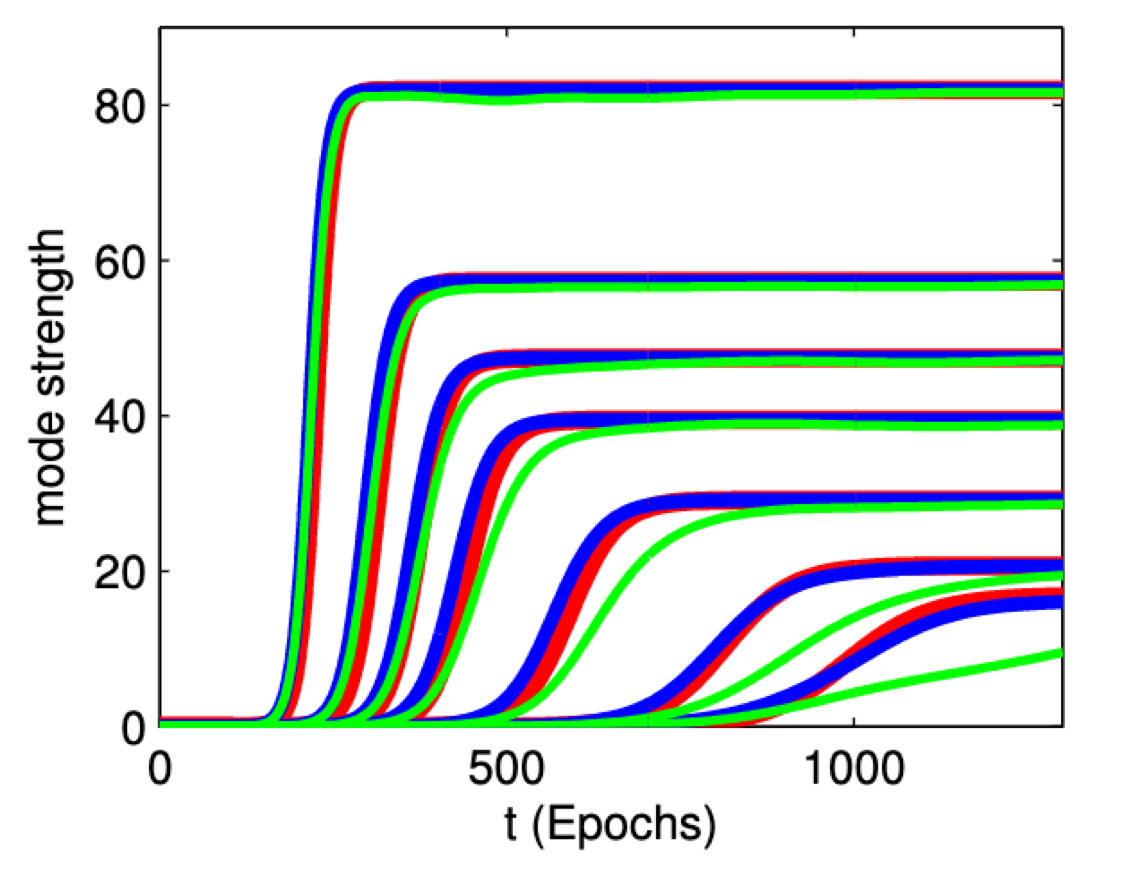
\includegraphics[width=0.5\textwidth]{Figs/dynamics_linear_network.jpeg}
    \caption{Dynamics of learning in a linear network}
    \label{fig:linear_network}
\end{figure}

%
%
%

\section{Shallow networks}

\subsection{Universal approximation theorem (simple version)}
We consider a neural network with a single hidden layer of N neurons: 
\begin{align*}
    \hat{y}(x) = W^2  \cdot \sigma(W^1 x + b)
\end{align*}
\begin{theorem}[Universal approximation theorem]\ \\
For every continuous real valued function $f(x)$ on a compact subset of $\mathbb{R}^d$ and every $\epsilon > 0$  
there exists $N \in \mathbb{N}$, $W^1, W^2 \in \mathbb{R}^N, b \in \mathbb{R}$ such that $\lVert f(x) - \hat{y}(x) \rVert < \epsilon$ for all $x$.
\end{theorem}

\begin{figure}
    \centering
    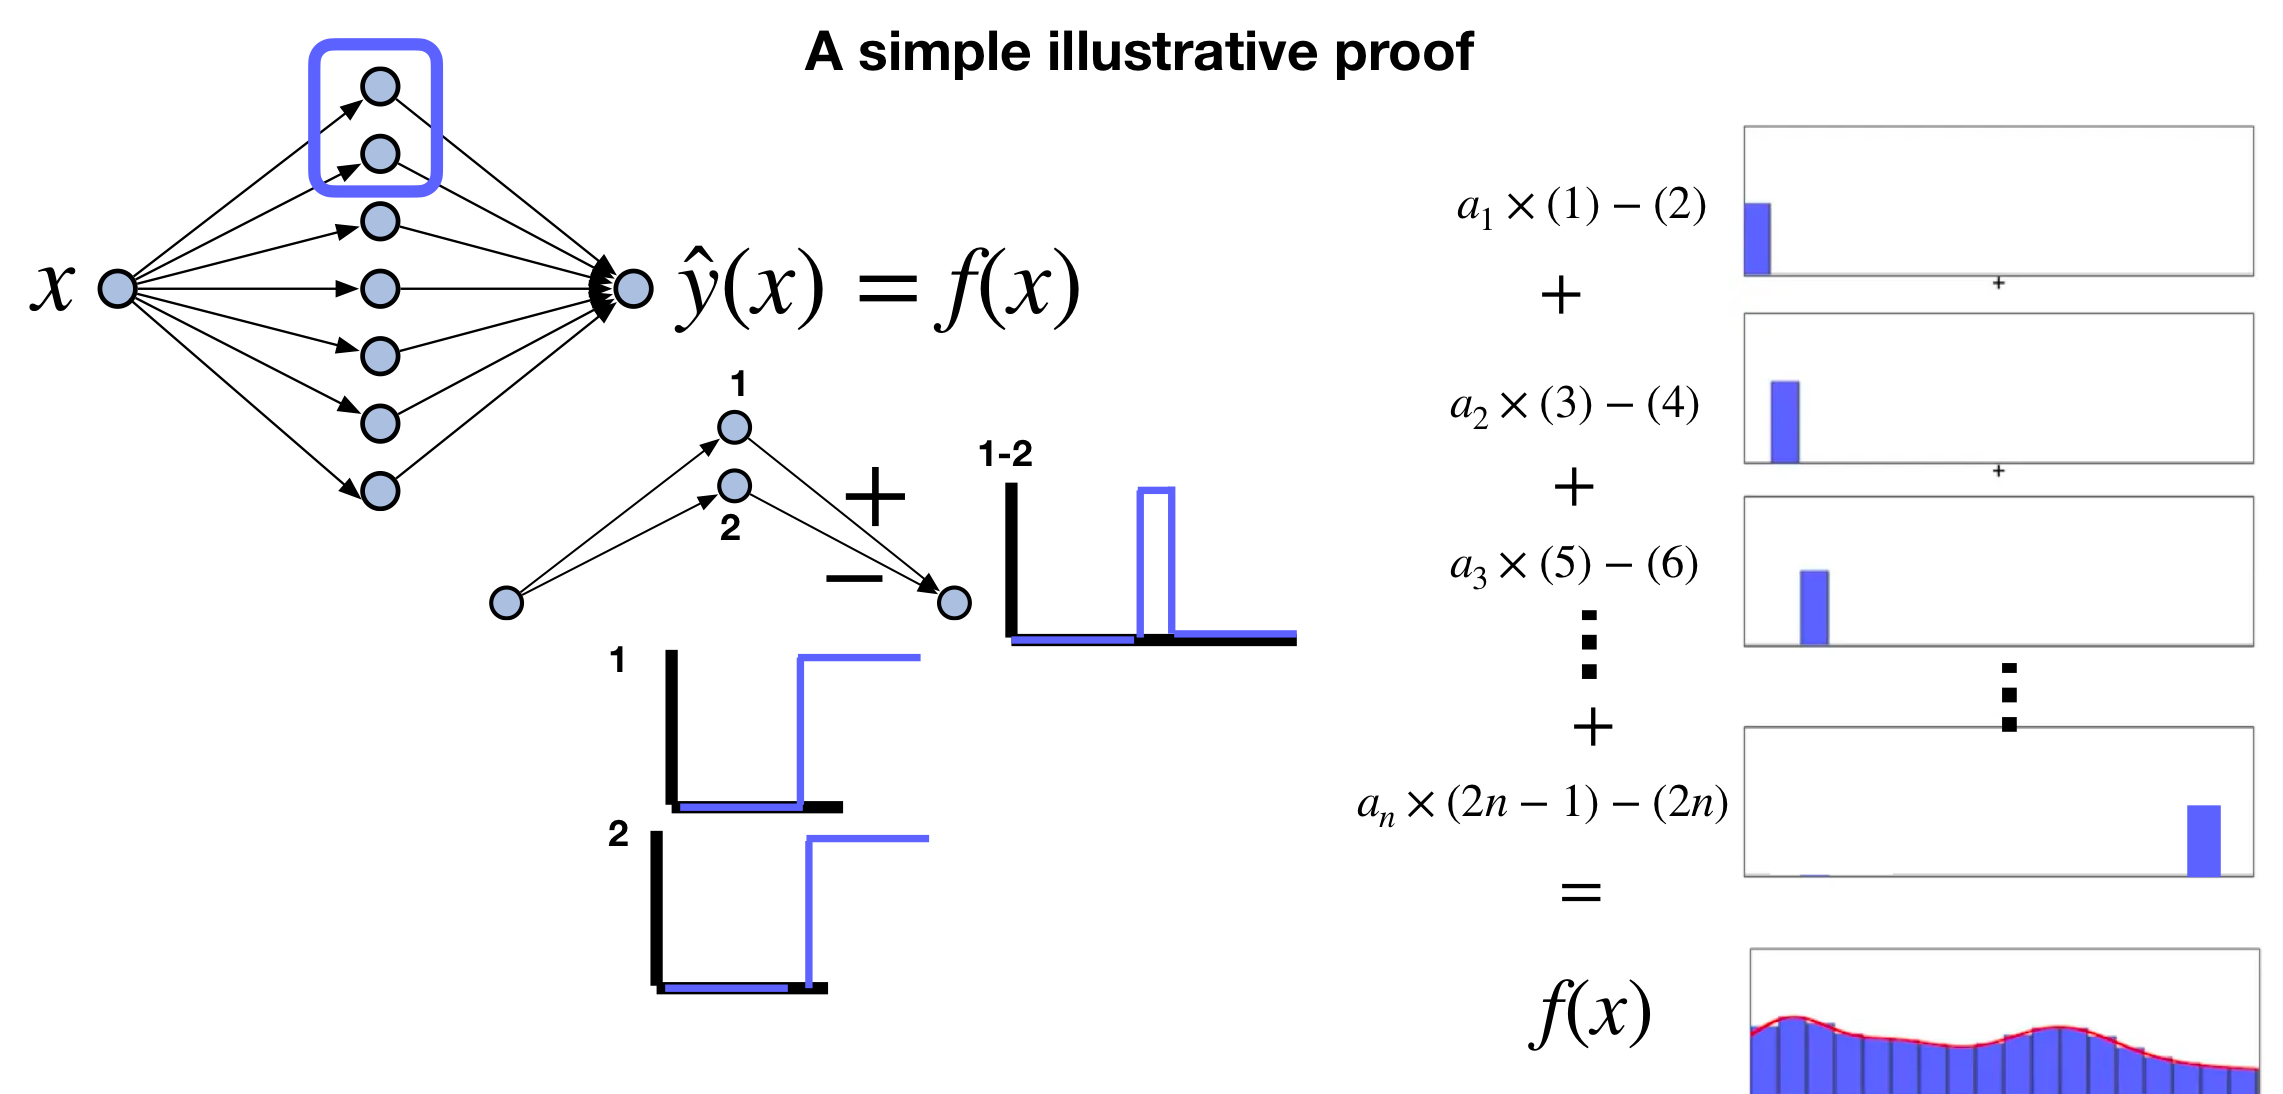
\includegraphics[width=0.9\textwidth]{Figs/universal_approx_thm.jpeg}
    \caption{Universal approximation theorem - intuition}
    \label{fig:universal_approximation}
\end{figure}


%
%

\subsection{Universal approximation theorem}

%
%

\subsection{Barron's theorem}

%
%

\subsection{The curse of dimensionality (Mhaskar)}

%
%
%

\section{Deep and shallow networks in the brain}

In the brain, there exists a hierarchical structure of deep computation, notably in the visual pathway, while the cerebellum exhibits a shallow but wide layering. 
This structure underpins the brain's powerful ability to process complex stimuli and learn from environmental interactions.

\begin{figure}[ht]
    \centering
    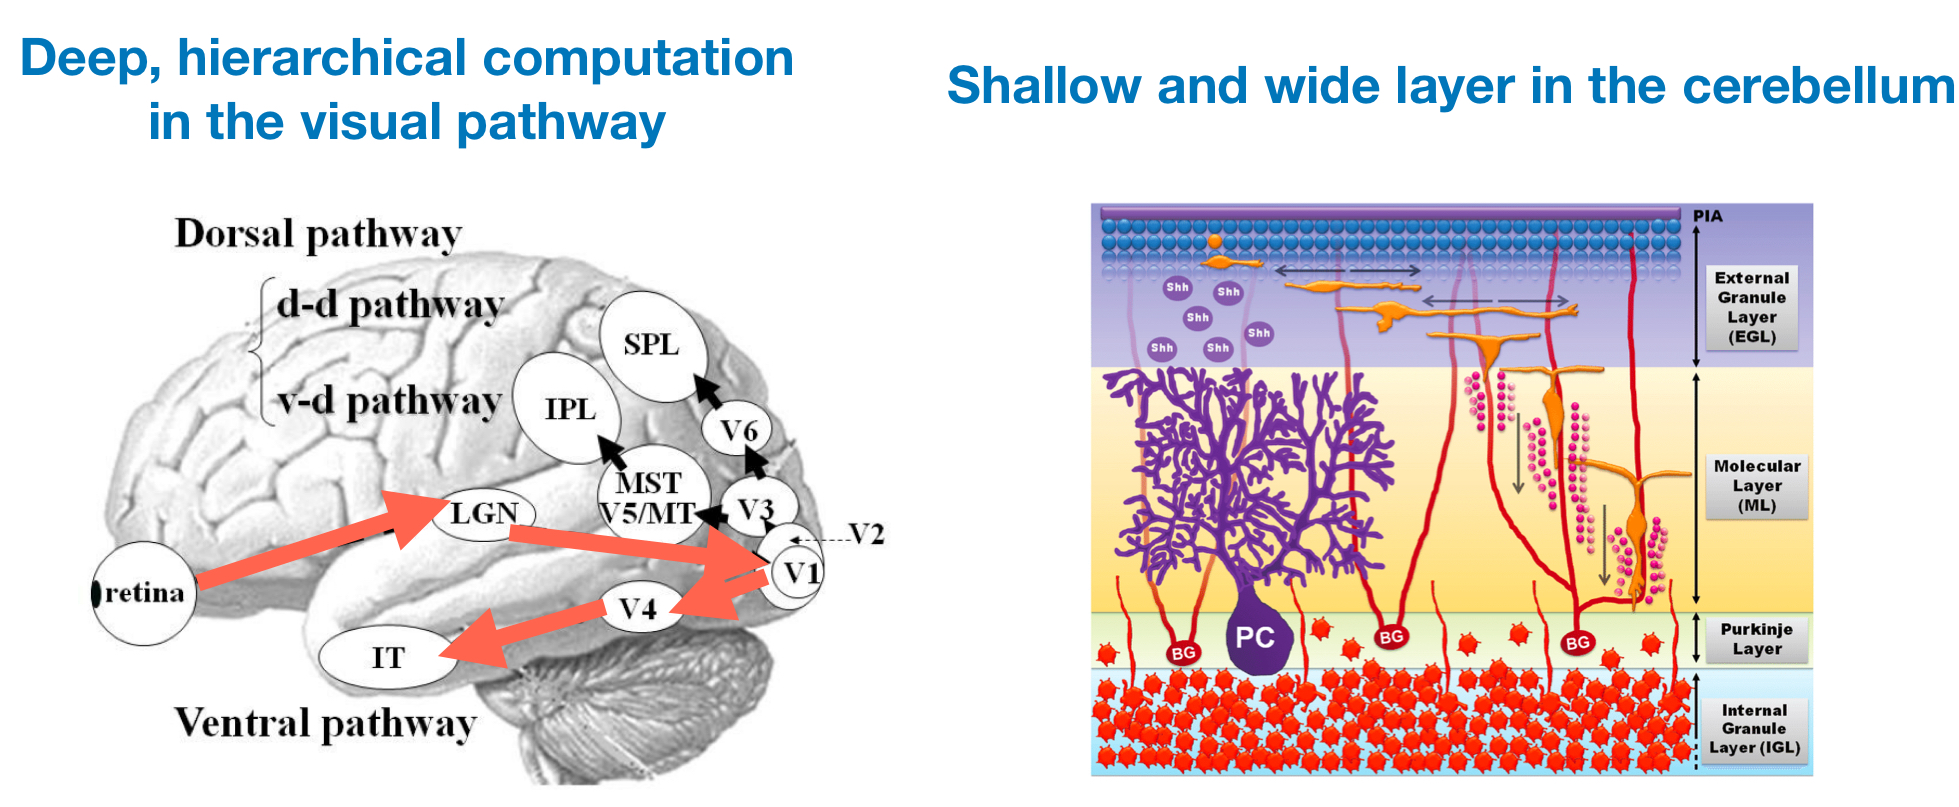
\includegraphics[width=\textwidth]{./Figs/deep_and_shallow_brain.jpeg}
    \caption{Deep and shallow networks in the brain}
    \label{fig:brain_networks}
\end{figure}

\section{Why go deep?}
Deep networks offer several advantages over their shallow counterparts, particularly in terms of expressivity and efficiency.

\subsection{Expressivity}
Expressivity refers to the network's ability to represent a wide variety of functions.

\subsubsection{Size efficiency of deep networks}
Deep networks are more size-efficient as they require fewer neurons to represent complex functions compared to shallow networks.
This efficiency is partly due to their hierarchical structure, which allows deep networks to reuse features and represent functions more compactly.

For example, a $\textbf{"sward-tooth"}$ function can be represented by a deep network with fewer neurons than a shallow network.
A $\approx 2^N$ neurons are required to represent the function in a shallow network, 
while a deep network can represent it with $\approx 3N$ neurons arranged in $\approx 2N$ layers.

\begin{figure}[ht]
    \centering
    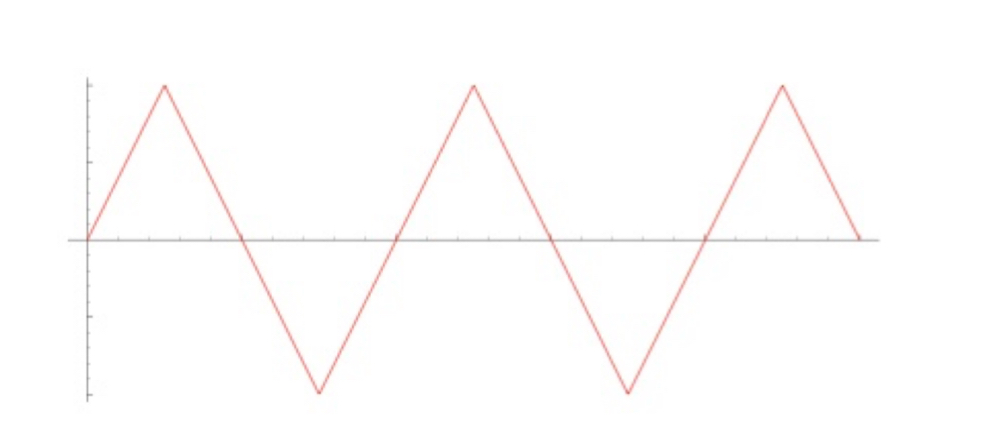
\includegraphics[width=0.4\textwidth]{./Figs/sward-tooth.jpeg}
    \caption{Sward-tooth function}
    \label{fig:size_efficiency_deep_networks}
\end{figure}

In $\textbf{"On the Number of Linear Regions of Deep Neural Networks"}$ by Montufar et al. (2014)
They showed that deep networks are able to sequentially map portions of each layer's input-space to the same output. 
In this way, deep models compute functions that react equally to complicated patterns of different inputs.
The compositional structure of these functions enables them to re-use pieces of computation exponentially often in terms of the network's depth. 

\begin{figure}[ht]
    \centering
    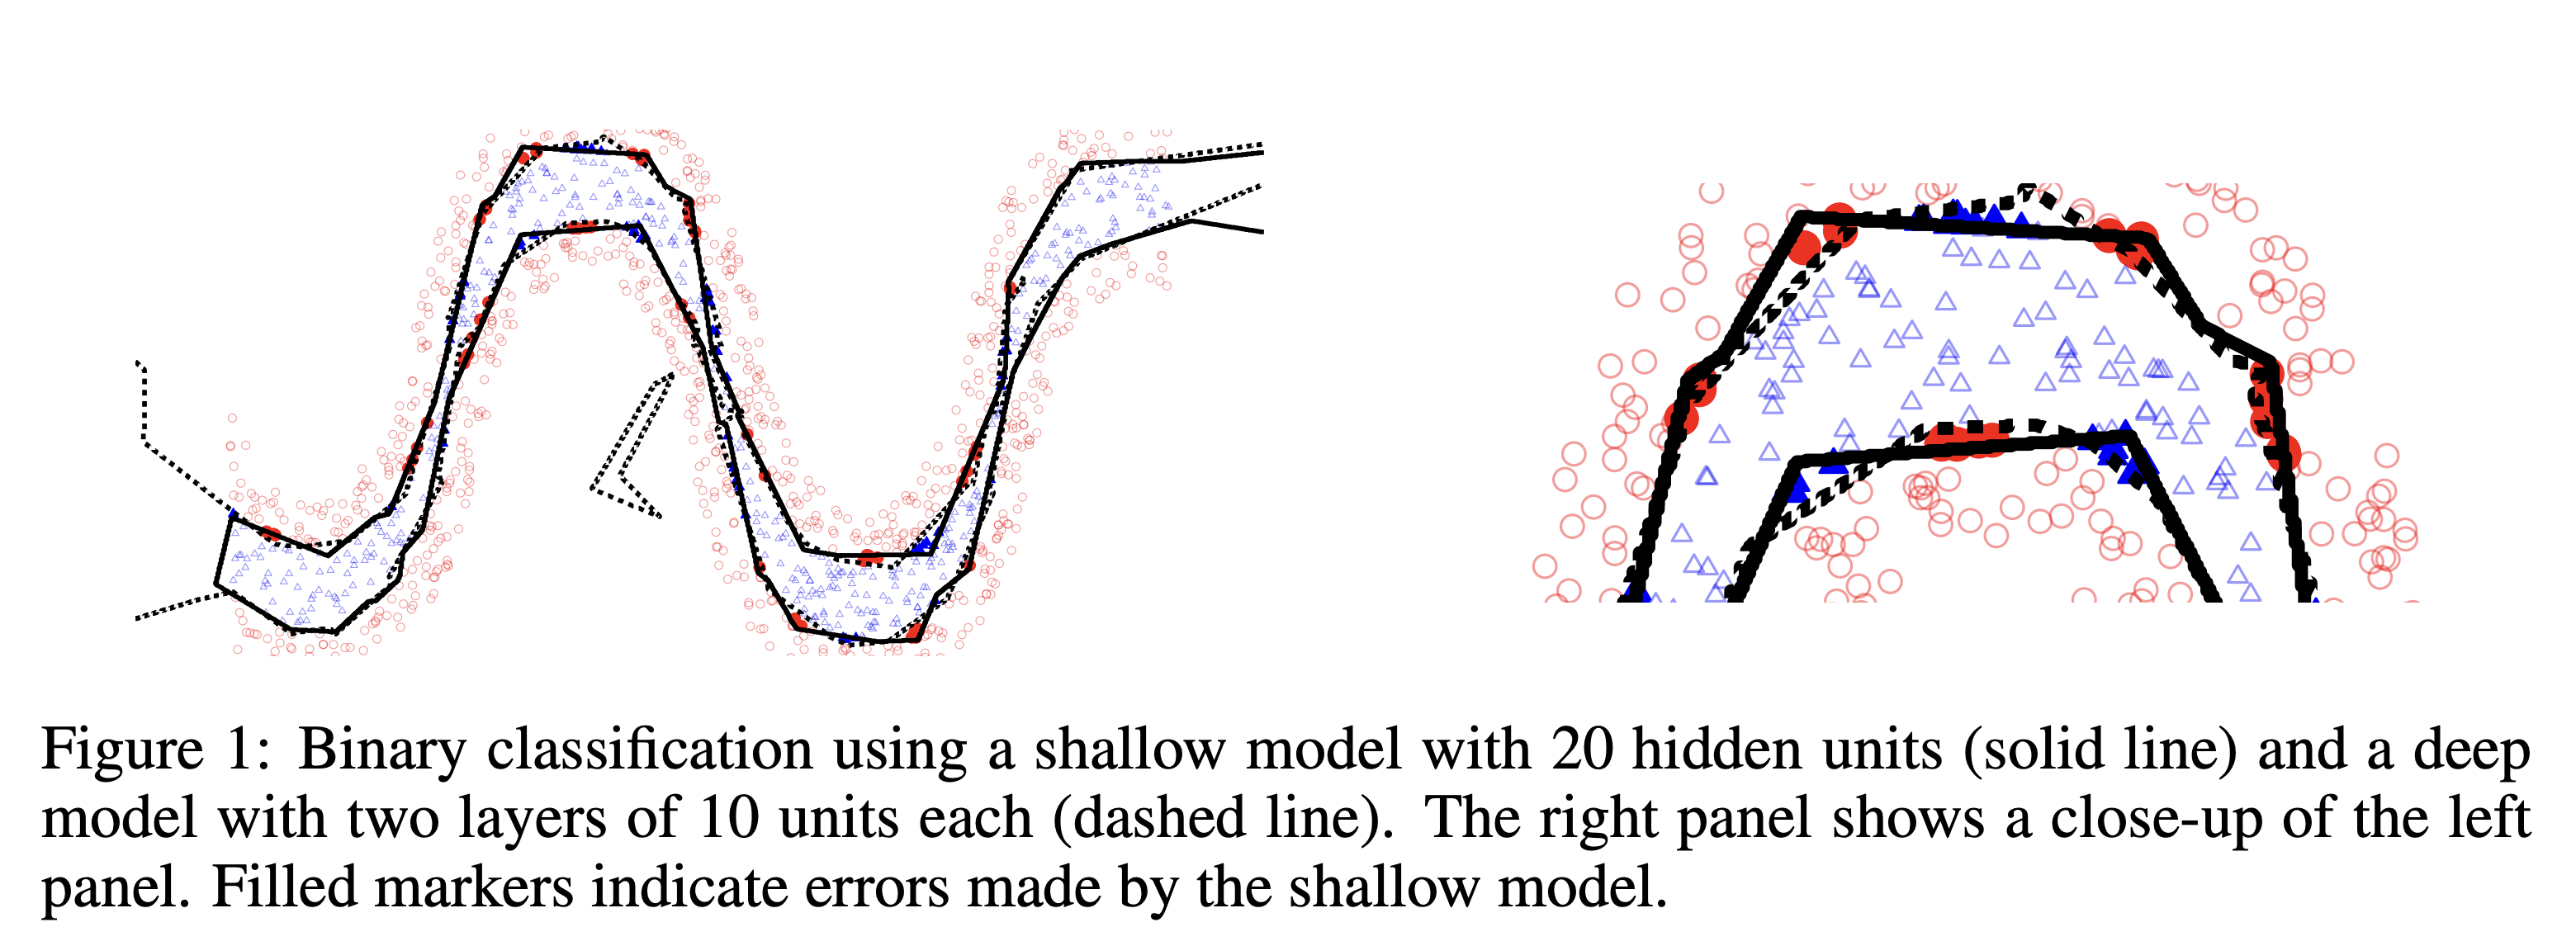
\includegraphics[width=\textwidth]{./Figs/piecewise_linear_function.png}
    \caption{Approximation by piecewise linear function and shallow networks}
    \label{fig:size_efficiency_deep_networks}
\end{figure}


\subsubsection{Exponential expressivity in deep networks}
As networks become deeper, their expressivity grows exponentially, not just adding but multiplying their ability to represent complex functions and interactions among inputs.

\begin{figure}[ht]
    \begin{subfigure}[b]{0.8\textwidth}
        \centering
        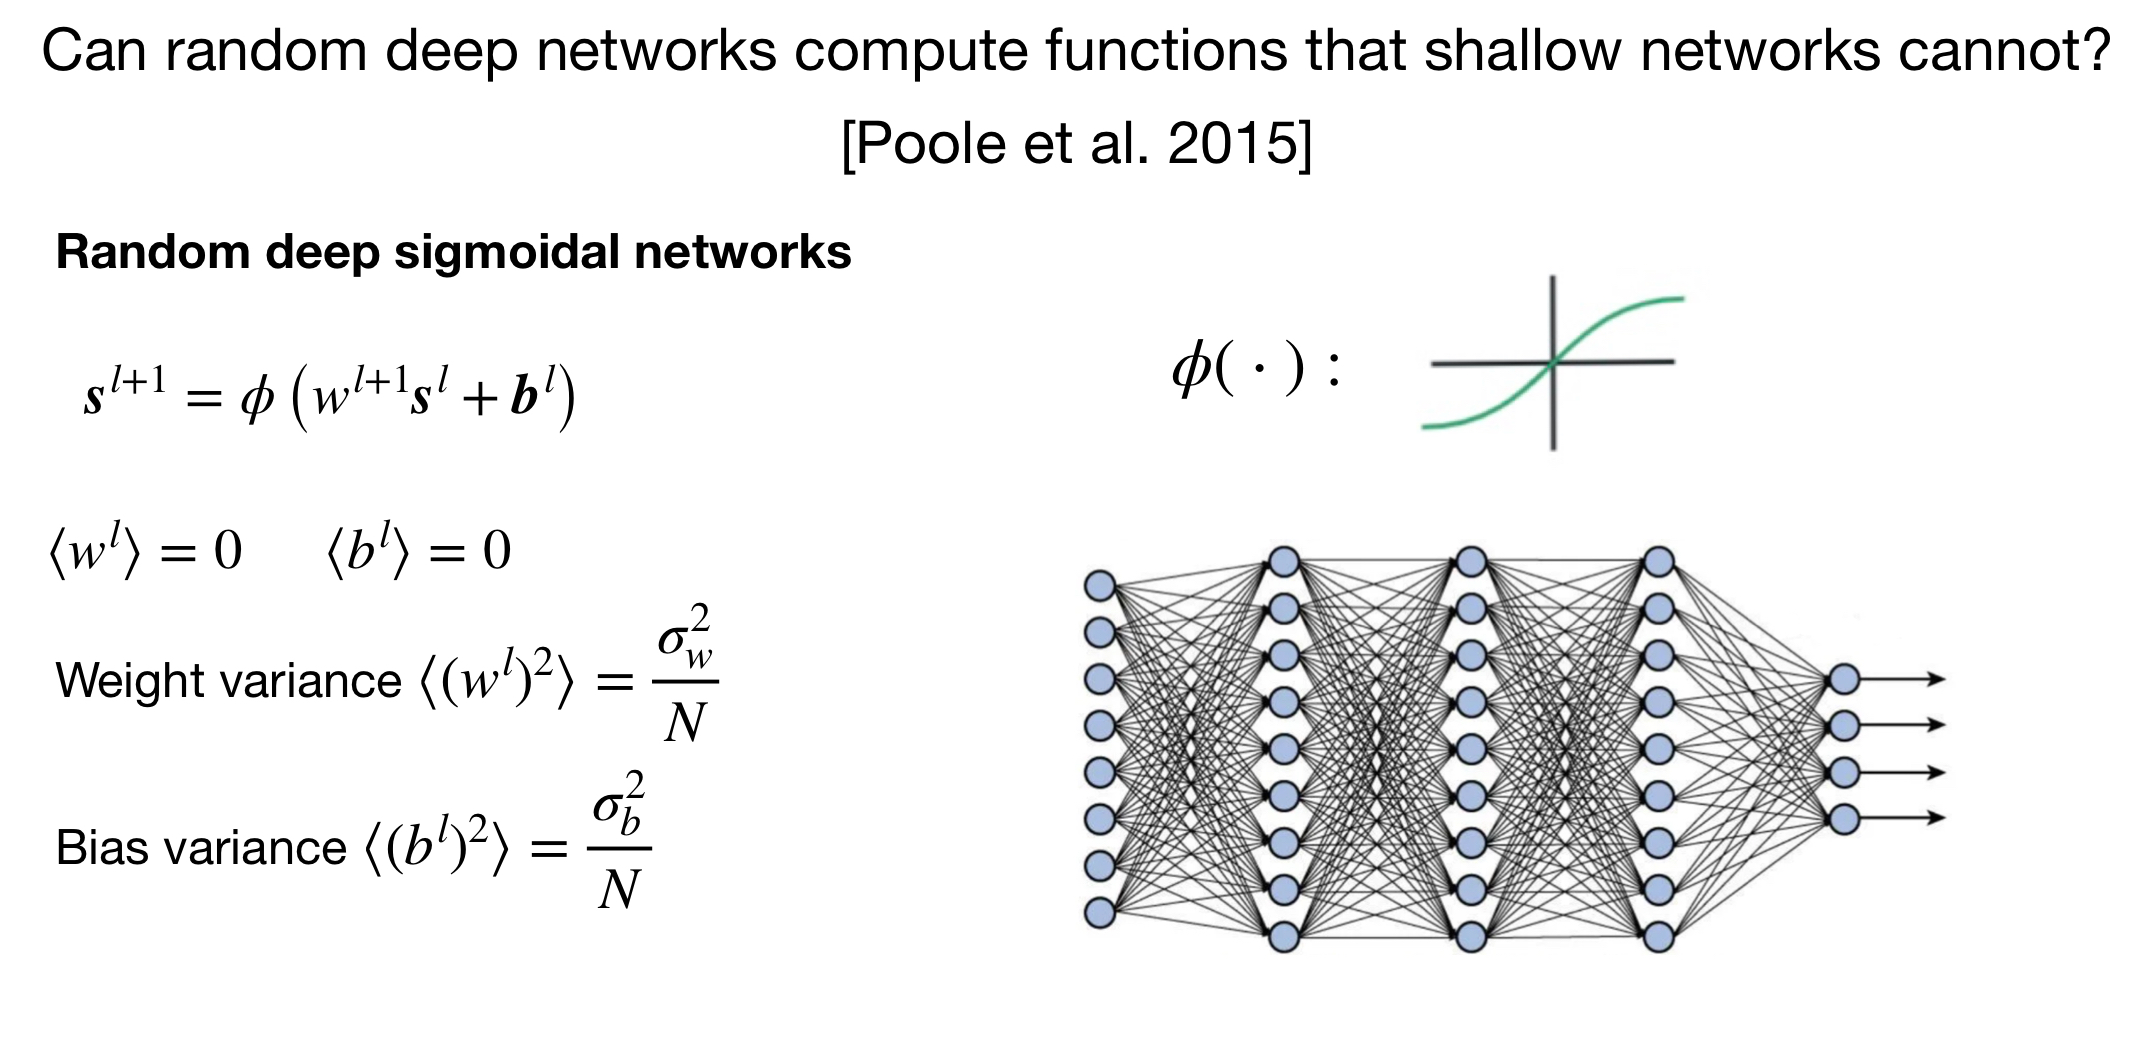
\includegraphics[width=\textwidth]{./Figs/expressivity1.jpeg}
        \label{fig:exponential_expressivity}
    \end{subfigure}
    \hfill
    \begin{subfigure}[b]{0.8\textwidth}
        \centering
        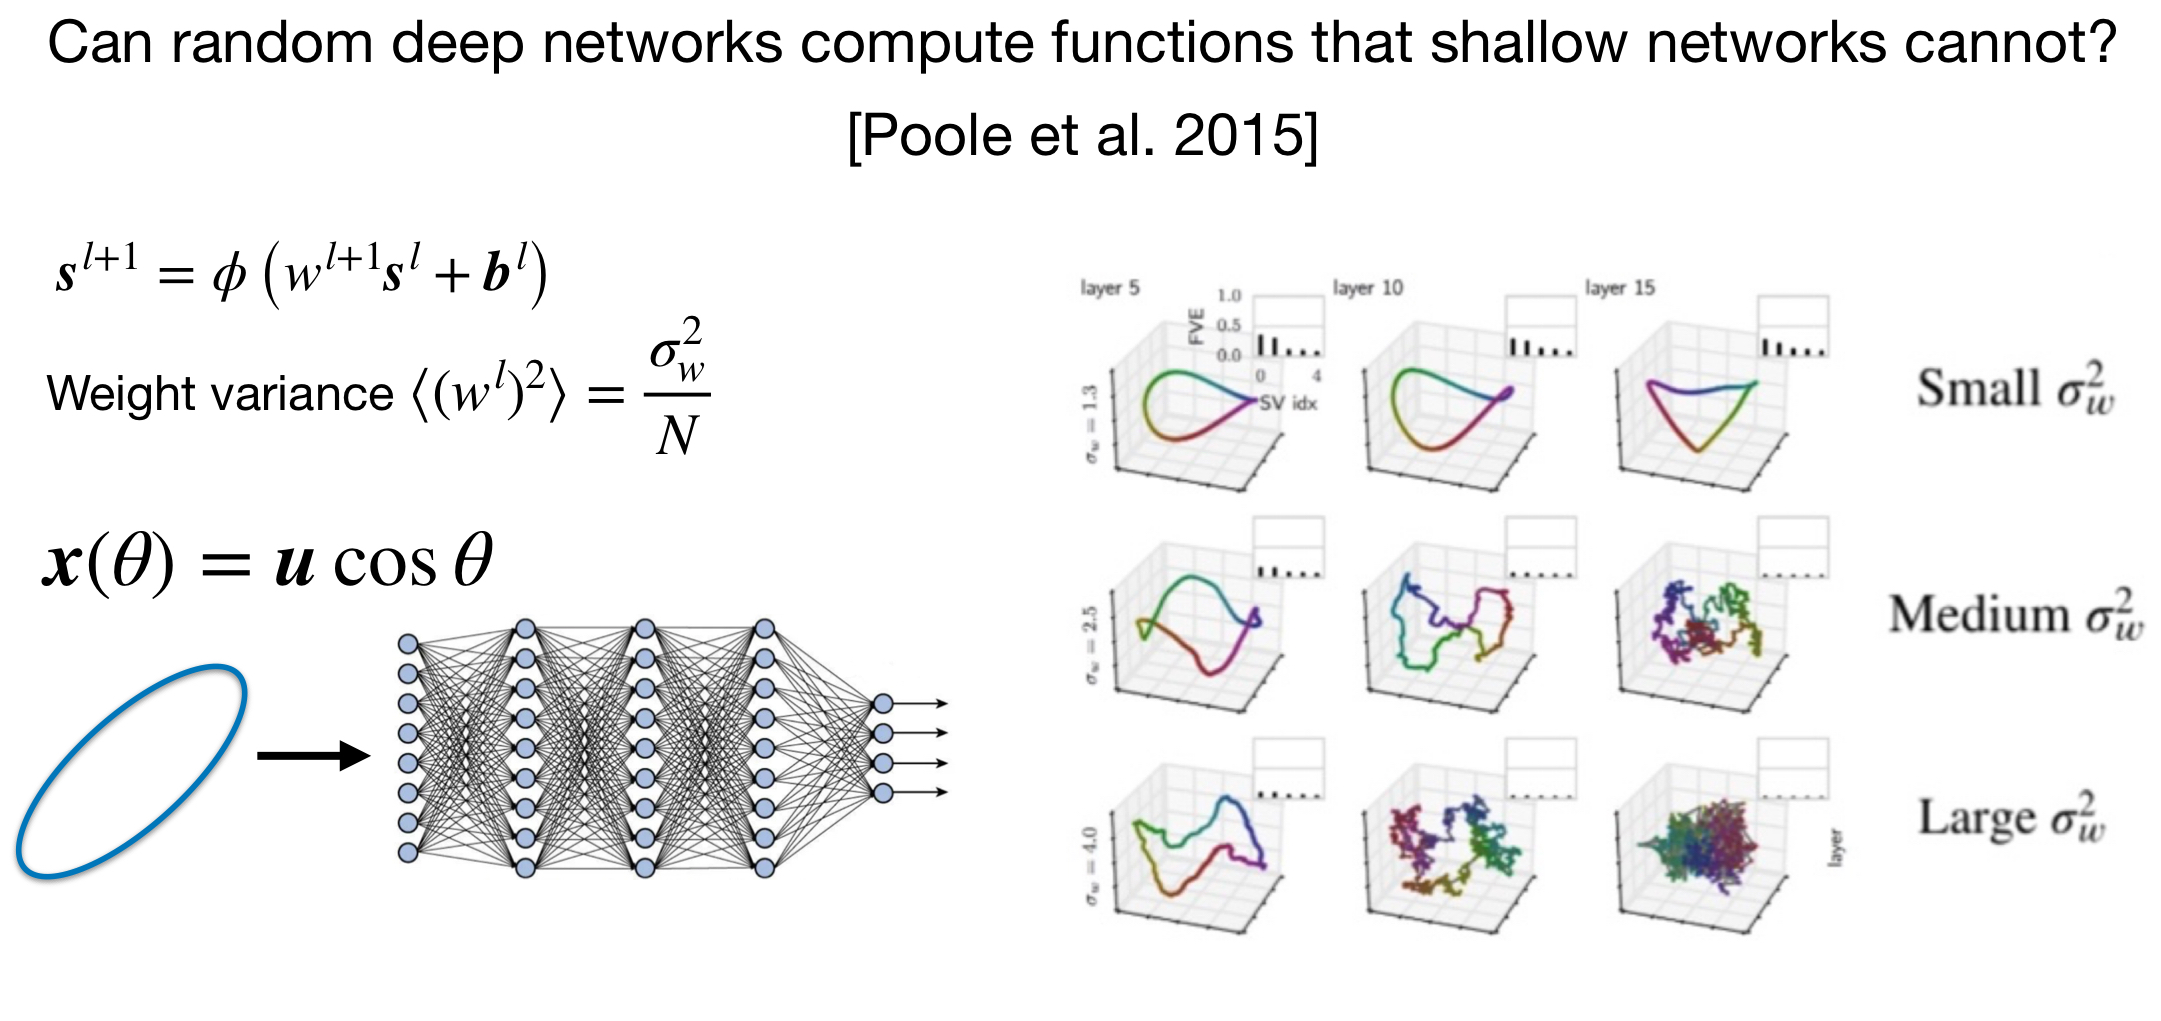
\includegraphics[width=\textwidth]{./Figs/expressivity2.jpeg}
        \label{fig:exponential_expressivity2}
    \end{subfigure}
    \caption{Exponential expressivity in deep networks, Poole et al. (2015)}
\end{figure}

\subsubsection{Manifold disentanglement}
Deep networks have the unique capability to disentangle complex data manifolds, making them more separable and thus easier to classify.
This ability is analogous to how the visual system in mammals processes and identifies objects across varying conditions.

\subsection{Trainability}
Trainability concerns the network's ability to adjust its parameters effectively through the learning process.

\subsubsection{Sample complexity (Training shallow vs deep networks)}
Deep networks generally have lower sample complexity, meaning they require fewer examples to learn the underlying distribution of the data. 
This attribute is vital for learning from limited data.
\begin{claim*}
    Wide networks can express deep representations on some data set, but they cannot learn it given the same sized data set.
\end{claim*}
\begin{figure}[ht]
    \begin{subfigure}[b]{0.6\textwidth}
        \centering
        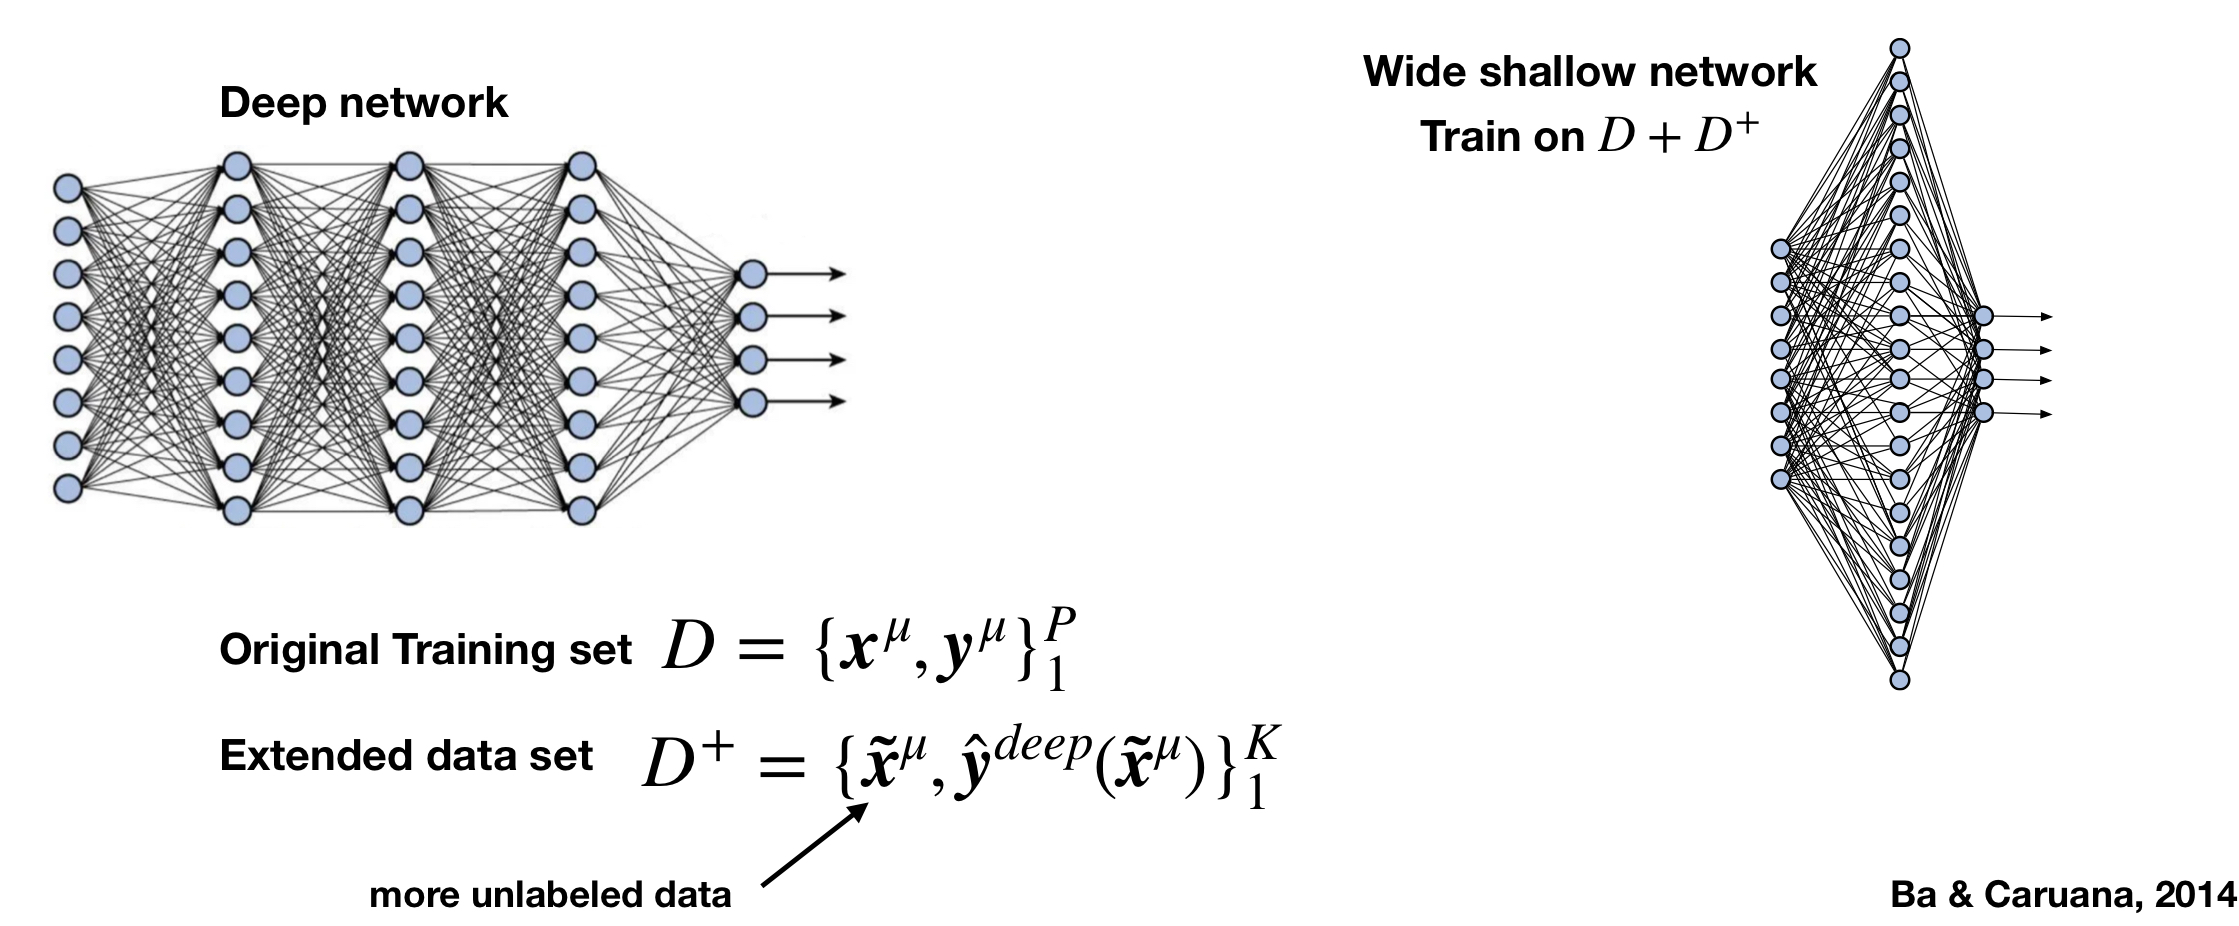
\includegraphics[width=\textwidth]{./Figs/deep_trainability2.jpeg}
        \label{fig:sample_complexity1}
    \end{subfigure}
    \hfill
    \begin{subfigure}[b]{0.33\textwidth}
        \centering
        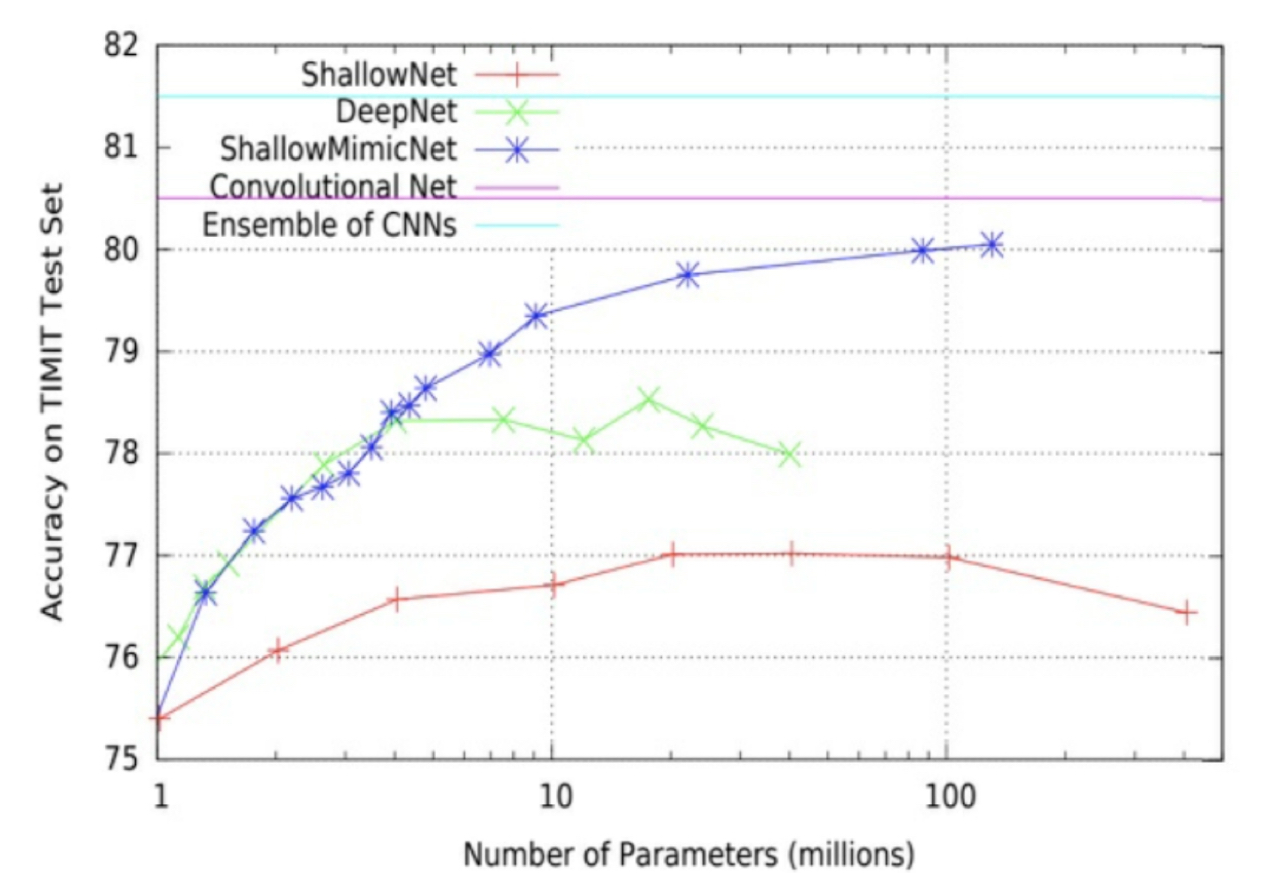
\includegraphics[width=\textwidth]{./Figs/deep_trainability1.jpeg}
        \label{fig:sample_complexity2}
    \end{subfigure}
    \caption{Deep vs shallow networks in terms of sample complexity}
\end{figure}

Shallow networks face challenges in training, especially as the complexity of the task increases. 
Deep networks, with their hierarchical structure, can learn more complex representations more efficiently.

\subsubsection{The importance of a good initialization}
Proper initialization of network weights is critical for the successful training of deep networks. 
Good initialization can prevent issues such as vanishing or exploding gradients and ensure that the network learns effectively.

\textcolor{red}{TODO}


\subsection{Generalization}
Generalization refers to the network's ability to perform well on unseen data.

\subsubsection{The overparameterized regime}
Deep networks often operate in an overparameterized regime where they have more parameters than necessary to fit the training data. 
Despite this, they are still able to generalize well, which is somewhat counterintuitive and a subject of ongoing research.

\textcolor{red}{TODO}


\subsubsection{Why are deep networks good at generalization?}
Despite their complexity and capacity, deep networks have shown remarkable generalization abilities,
 which is theorized to be due to properties such as flat minima in their loss landscapes, among other factors.

\section{Visual processing in the brain}
The brain processes visual information through a hierarchical pathway, involving several stages of transformation and representation.

\begin{figure}[ht]
    \centering
    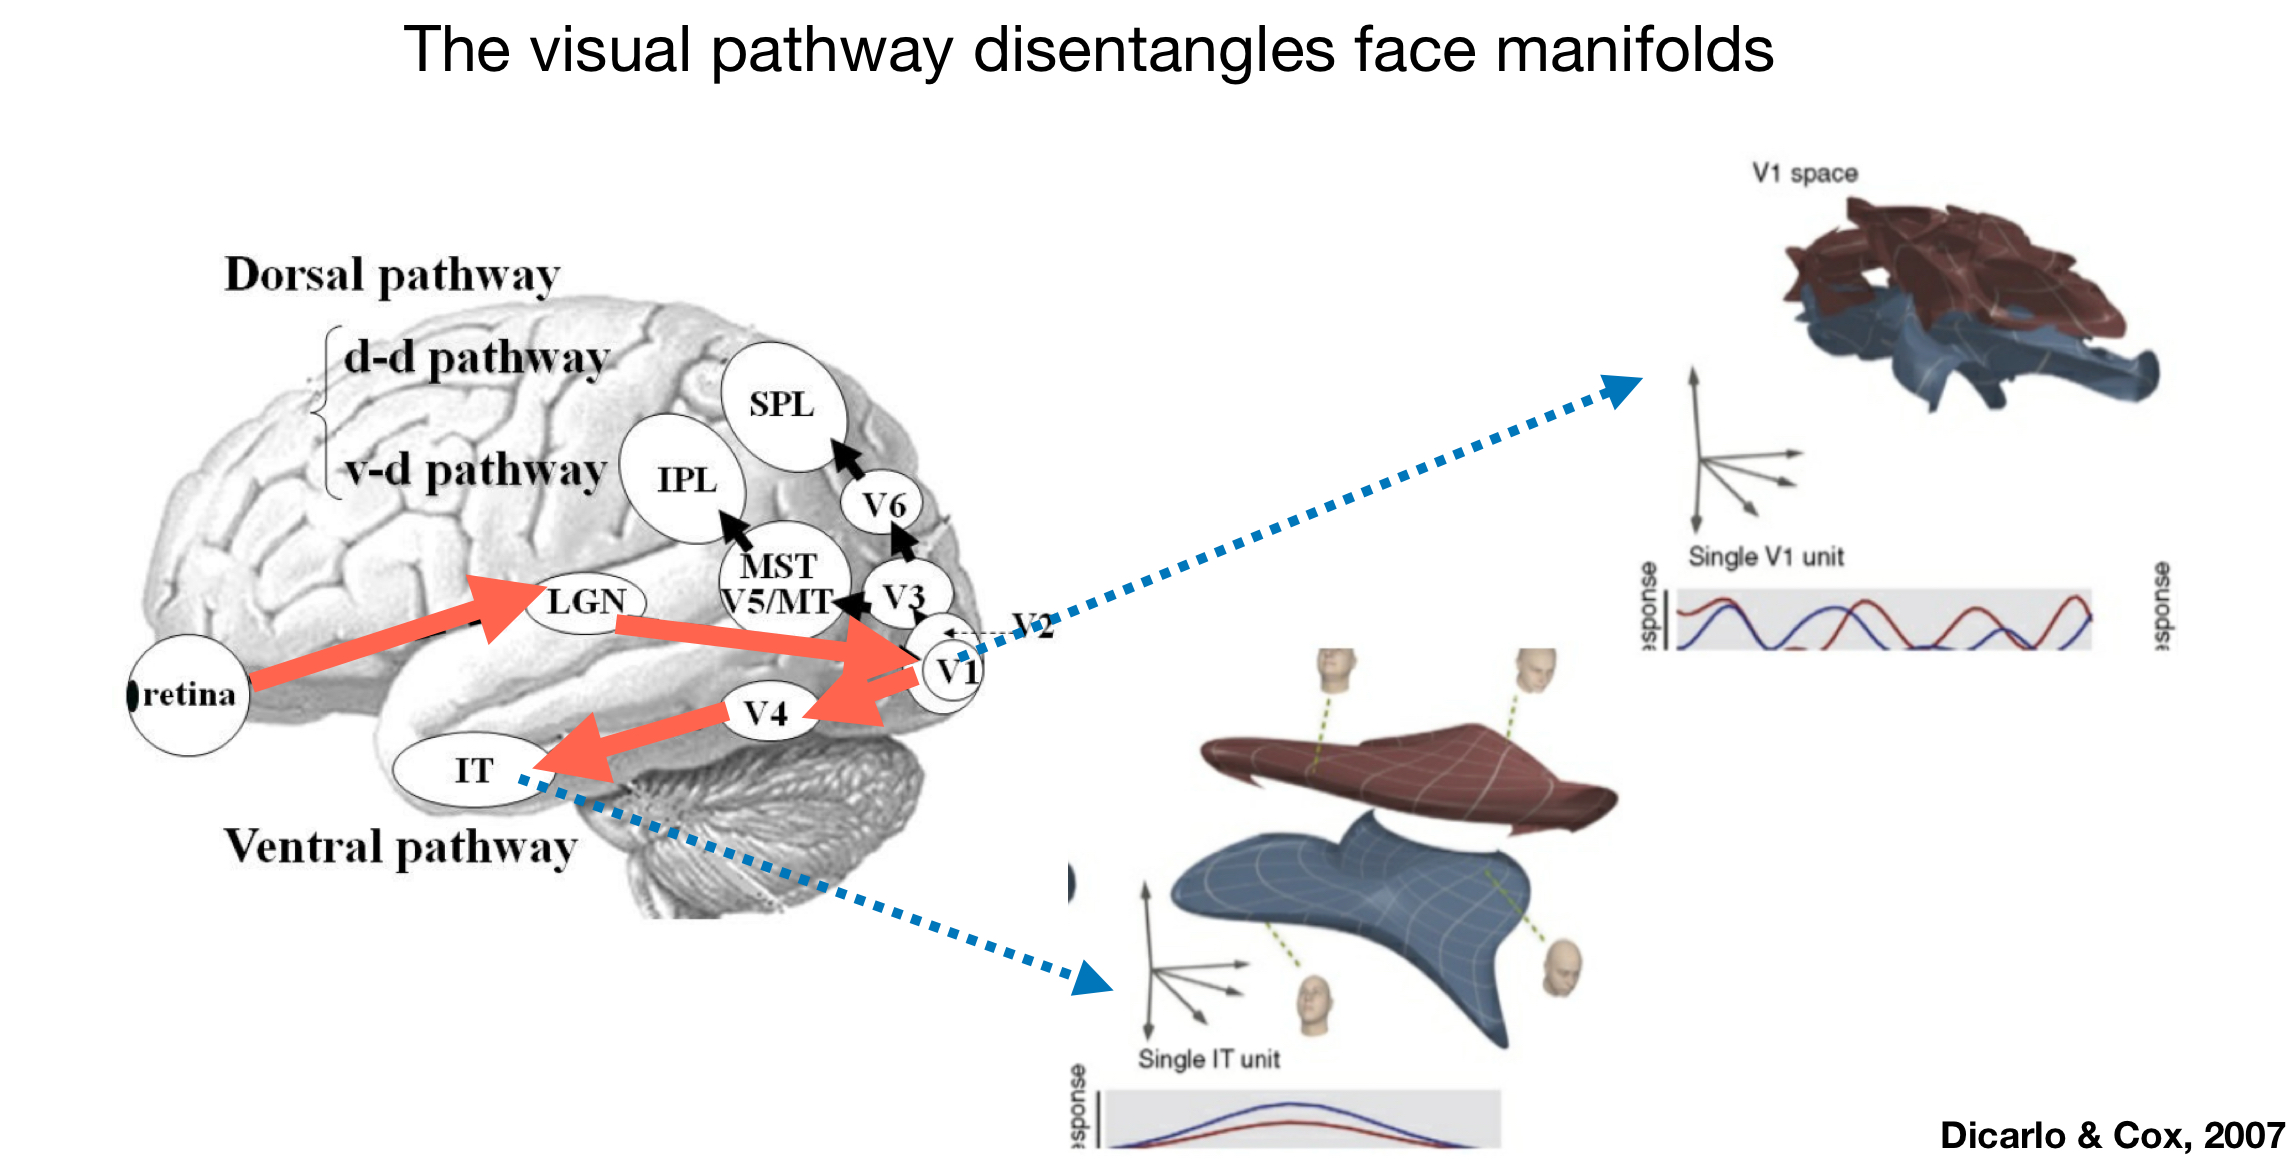
\includegraphics[width=\textwidth]{./Figs/visual_pathway_manifold.jpeg}
    \caption{The visual pathway disentangles complex data manifolds.}
    \label{fig:visual_pathway}
\end{figure}

\subsection{The visual pathway}
The visual pathway consists of a series of areas, each building upon the previous ones' outputs to create increasingly abstract representations of the visual input.
The ventral path pathway consists of the following areas:
\begin{itemize}
    \item retina: The first stage of visual processing, where light is converted into neural signals.
    \item LGN: Lateral geniculate nucleus of the thalamus 
    \item V1: Primary visual cortex
    \item V2: Secondary visual cortex
    \item V4: Visual area 4
    \item IT: Inferior temporal cortex
\end{itemize}

\subsection{The visual cortex}
Within the visual cortex, processing begins with simple features like edges and progresses to complex object representations, 
demonstrating a form of deep, hierarchical computation.

\subsection{The receptive field}
Each neuron in the visual system has a receptive field, an area of the visual field to which it responds. 
As visual information flows through the pathway, the receptive fields become larger and more selective, enabling the recognition of complex patterns.



%
%
%
%
%
%
%
%
%
%
%
%
%
%
%
%


\chapter{Recurrent Neural Networks}

\section{Circuit equations for RNNs}


\subsection{The dynamics of a single neuron in a discrete time}
Output of a neuron is given by:
\[
    s_i(t) = \phi(h_i(t))
\]
Point neuron (in time) is given by:
\[
    h_i(t + \bigtriangleup  t) = (1 - \bigtriangleup t) h_i(t) + \bigtriangleup t (\sum_{j=1}^N W_{ij} s_j(t) + u_ix(t))
\]
Where:
\begin{itemize}
    \item $h_i(t)$ is the membrane potential of the neuron $i$ at time $t$
    \item $s_i(t)$ is the output of the neuron $i$ at time $t$
    \item $\phi$ is the activation function
    \item $W_{ij}$ is the weight of the connection to neuron $i$ from neuron $j$
    \item $u_i$ is a vector of weights that connect the neuron to the external input
    \item $x(t)$ is the external input at time $t$
    \item $\bigtriangleup t$ is the time step
    \item $N$ is the total number of neurons in the network
\end{itemize}

\subsection{The dynamics of a RNN in a continuous time}
Consider a neural network with $N$ neurons with connectivity matrix $J \in \mathbb{R}^{N \times N}$, and external input $x(t) \in \mathbb{R}^N$.
The dynamics of the network are given by:
\[
    \frac{dh_i(t)}{dt} = -h_i(t) + \sum_{j=1}^N J_{ij} \phi(h_j(t)) + w_i^{in} I(t)
\]

and the output of the network is given by:
\[
    z(t) = \sum_{j=1}^N \nu_j \phi(h_j(t))
\]
Where:
\begin{itemize}
    \item $w_i$ is the input weights vector of the neuron $i$
    \item $h_j(t)$ is the membrane potential of the neuron $j$ at time $t$
    \item $\phi$ is the activation function
    \item $\nu_j$ is the readout weight of the neuron $j$
\end{itemize}

\begin{figure}
    \centering
    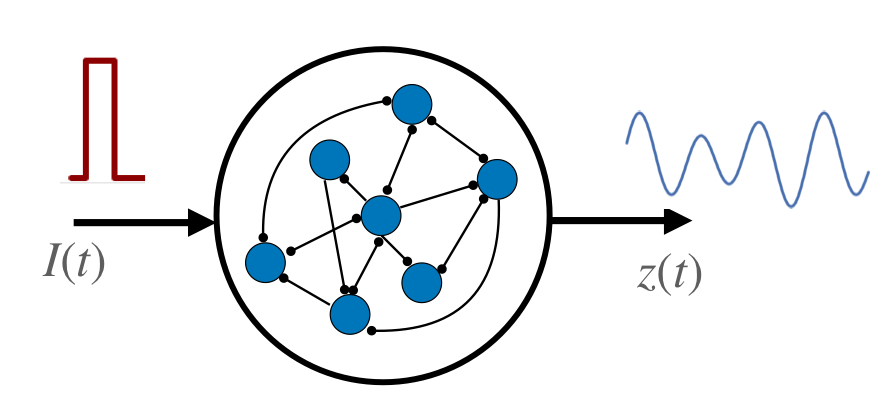
\includegraphics[width=0.6\textwidth]{Figs/RNN.jpeg}
    \caption{Recurrent Neural Network}
    \label{fig:rnn}
\end{figure}

\subsection{Examples of tasks solved with RNNs}

\section{Learning in RNNs}

Recurrent Neural Networks (RNNs) exhibit rich dynamics suitable for sequential data processing. 
Training RNNs, however, poses challenges due to the recurrent feedback of errors, amplifying them and complicating convergence, 
as well as making the credit assignment problem more difficult.

\subsection{Reservoir Computing}
In reservoir computing, the network is trained using the error of a linear readout of the units. 
This approach avoids the difficulties of training the entire network by only adjusting the readout weights.

\subsubsection{Open Circuit}
In an open circuit configuration, the network's output is not fed back during learning, preventing the amplification of initial errors. 
Instead, we make sure that we have the necessary ingredients to learn the output function by supplying the network with the desired output.
The dynamics of the network is given by:
\[
    \frac{dh_i(t)}{dt} = -h_i(t) + \sum_{j=1}^N J_{ij} \phi(h_j(t)) + w_i^{in} I(t) + u_i f(t)
\]
Once the network has been trained, we stop feeding it the target.
But without feeding the network with the target, the network is different from the one we trained.
Luckily, we have a good estimate of the output function $f(t) \approx z(t)$.

\begin{figure}[ht]
\centering
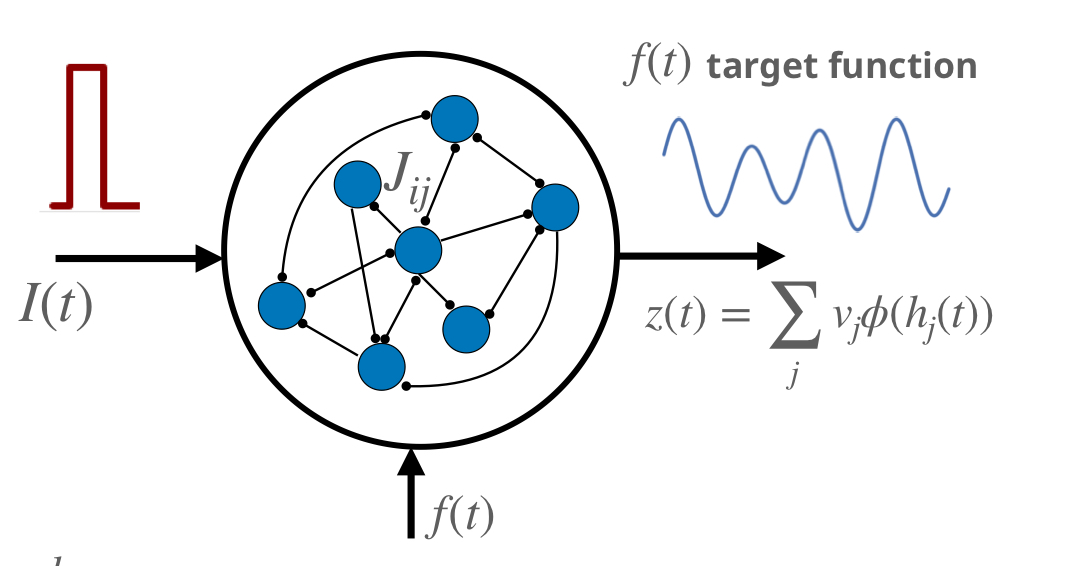
\includegraphics[width=0.6\textwidth]{Figs/RNN_open_circuit.jpeg}
\caption{Open circuit training of RNN.}
\label{fig:rnn_learning}
\end{figure}


\subsubsection{Closed Circuit (Echo/Liquid State Machines)}
In closed circuits, such as echo-state machines and liquid state machines, the output can be fed back into the network. 
If the network is trained properly, there is little to no difference from the open circuit.
The added solution is equivilent to a low-rank addition to $J_{ij}$.
The dynamics of the network is given by:
\begin{align*}
    \frac{dh_i(t)}{dt} = -h_i(t) + \sum_{j=1}^N J_{ij} \phi(h_j(t)) + w_i^{in} I(t) + u_i z(t) = \\
    -h_i(t) + \sum_{j=1}^N J_{ij} \phi(h_j(t)) + w_i^{in} I(t) + \sum_{j=1}^N u_i \nu_j \phi(h_j(t)) = \\
    -h_i(t) + \sum_{j=1}^N (J_{ij} + u_i \nu_j) \phi(h_j(t)) + w_i^{in} I(t) = \\
    -h_i(t) + \sum_{j=1}^N \tilde{J}_{ij} \phi(h_j(t)) + w_i^{in} I(t)
\end{align*}
Where: $\tilde{J}_{ij} = J_{ij} + u_i \nu_j$

\begin{figure}[ht]
\centering
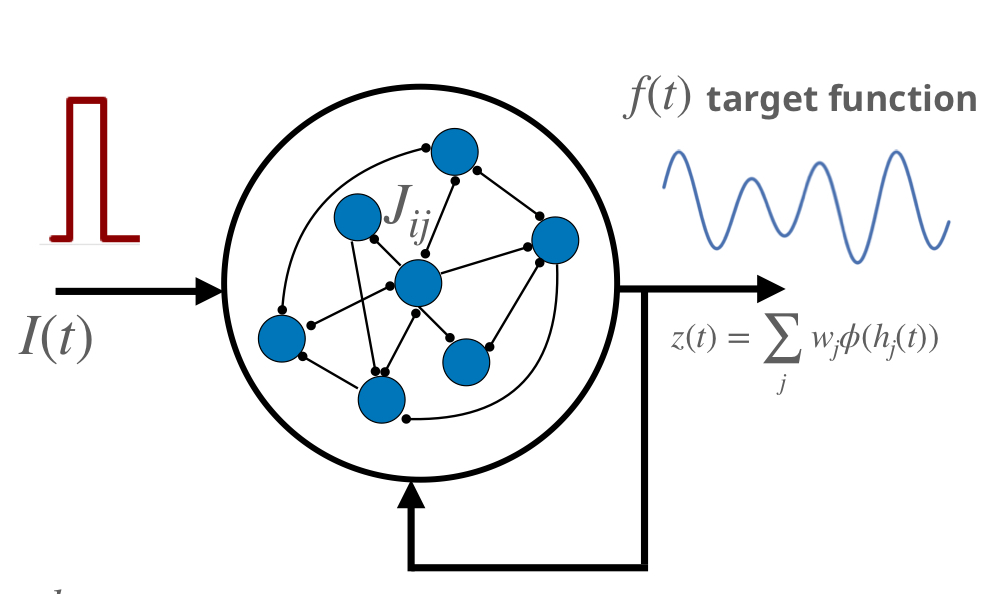
\includegraphics[width=0.6\textwidth]{Figs/RNN_closed_circuit.jpeg}
\caption{Closed circuit RNN.}
\label{fig:rnn_learning}
\end{figure}

\subsection{Recursive Least Squares (RLS)}
Recursive Least Squares (RLS) is a fast algorithm for linear regression over sequential data, 
minimizing a weighted linear least squares cost function. 
It is particularly well-suited for scenarios where parameters must be rapidly adjusted in response to evolving data streams.

\subsection{FORCE Learning (RLS on the Output Function)}
FORCE (First-Order Reduced and Controlled Error) learning is a closed-circuit training method for RNNs. 
In this approach, the output of the network can be fed back as input during the training process. 
Unlike open-circuit models, which do not feed the output back into the network during training,
FORCE learning leverages the feedback to adjust the synaptic weights quickly and effectively, reducing the magnitude of the output error. 

\subsubsection{Derivation}
RLS for FORCE learning is derived by minimizing a regularized weighted least squares cost function that accounts for the error at each time step 
and incorporates a discounting factor for older signals.
Consider an RNN with a readout that is defined at time t for every $t' < t$ as:
\[
    z(t') = \vec{w}(t) \cdot \vec{\phi} (h(t'))
\]
Given a sequence of signals $\{\vec{x}\}^t \subset \mathbb{R}^N$ we aim to learn weights $\vec{w}^*(t)$ that best approximate some target $f(t) = f(\{\vec{x}\}^t)$.
The error at time t' is given by:
\[
    \epsilon(t') = f(t') - z(t')
\]
We will define the weighted least squares cost function as:
\[
    L(\vec{w}(t)) = \sum_{t'=1}^t \lambda^{t-t'} \epsilon^2(t') + \alpha \lambda^t \lVert \vec{w}(t) \rVert^2
\]
Where:
\begin{itemize}
    \item $0 < \lambda \leq 1$ is the discounting factor
    \item $\alpha$ is the regularization parameter
\end{itemize}

The minimum of L w.r.t $\vec{w}(t)$ is given by:

\begin{align*}
   &0 = \frac{\partial L}{\partial {w_i}} = 2 \sum_{t'=1}^t \lambda^{t-t'} \epsilon(t') \frac{\partial \epsilon(t')}{\partial w_i} + 2 \alpha \lambda^t {w_i}(t) \\
   &(
        \frac{\partial \epsilon(t')}{\partial {w_i}} = 
        \frac{\partial f(t')}{\partial {w_i}} - \frac{\partial z(t')}{\partial {w_i}} =
        - \frac{\partial z(t')}{\partial {w_i}} =
        - \phi_i (t')
    ) \\
   &0 = - \sum_{t'=1}^t \lambda^{t-t'} \epsilon(t') \phi_i(t') + \alpha \lambda^t w_i(t) \\
   &0 = - \sum_{t'=1}^t \lambda^{t-t'} (f(t') - z(t')) \phi_i(t') + \alpha \lambda^t w_i(t) \\
   &0 = - \sum_{t'=1}^t \lambda^{t-t'} (f(t') - \vec{w}(t) \cdot \vec{\phi}(t')) \phi_i(t') + \alpha \lambda^t w_i(t) \\
   &0 = - \sum_{t'=1}^t \lambda^{t-t'} f(t') \phi_i(t') + \sum_{t'=1}^t \lambda^{t-t'} \sum_{j=1}^N w_j(t) \phi_j(t') \phi_i(t') + \alpha \lambda^t w_i(t) \\
   &\sum_{t'=1}^t \lambda^{t-t'} f(t') \phi_i(t') = \sum_{j=1}^N  \left[ \sum_{t'=1}^t \lambda^{t-t'} \phi_j(t') \phi_i(t') + \alpha \lambda^t \delta_{ij} \right] w_j^*(t) \\
   &(M_{ij}(t) \stackrel{\text{def}}{=}   \sum_{t'=1}^t \lambda^{t-t'} \phi_j(t') \phi_i(t') + \alpha \lambda^t \delta_{ij}
   & {u_i}(t) \stackrel{\text{def}}{=}   \sum _{t'=1}^t \lambda^{t-t'} f(t') \phi_i(t')) \\
   &\sum _{j=1}^N M_{ij}(t) w_j^*(t) = u_i(t) \\
   &M(t) \vec{w}^* = \vec{u}(t) \rightarrow \vec{w}^* = (M(t))^{-1} \vec{u}(t)
\end{align*}

This approach entails inverting the matrix M numerically every time step, which can be computationally expensive.
We can see that we get similar result to Linear Regression solution but with a discounting factor, 
where $M(t)$ behaves like the feature covariance matrix $C_{tr}$ and $u(t)$ behaves like the input-output covariance vector $\vec{U_{tr}}$.

\subsubsection{Recursive Form of the Accumulative Covariance Matrix}
The accumulative covariance matrix, essential for updating the weights in RLS, can be computed recursively, allowing for efficient updates as new data arrives.
In the recursive form, the accumulative covariance matrix is given by:
\begin{align*}
    M_{ij}(t) = \sum_{t'=1}^t \lambda^{t-t'} \phi_i(t') \phi_j(t') =  \sum_{t'=1}^{t-1} \lambda^{t-t'} \phi_i(t') \phi_j(t') + \phi_i(t) \phi_j(t) \\
    {u_i}(t) = \sum _{t'=1}^t \lambda^{t-t'} f(t') \phi_i(t') = \sum _{t'=1}^{t-1} \lambda^{t-t'} f(t') \phi_i(t') + f(t) \phi_i(t)
\end{align*}
In the matrix form, the recursive update rule for the accumulative covariance matrix is given by:
\begin{align*}
    M(t) = \lambda M(t-1) + \vec{\phi}(t) \vec{\phi}(t)^T \\
    \vec{u}(t) = \lambda \vec{u}(t-1) + f(t) \vec{\phi}(t)
\end{align*}

We will define $P(t) \stackrel{\text{def}}{=} M^{-1}(t)$ and we will have:
\begin{align*}
    M^{-1}(t) =  P(t) = \frac{1}{\lambda} \left[ P(t-1) - \frac{P(t-1) \vec{\phi}(t) \vec{\phi}(t)^T P(t-1)}{\lambda + \vec{\phi}(t)^T P(t-1) \vec{\phi}(t)} \right]
\end{align*}

\subsubsection{Weights Update Rule}
The weights in FORCE learning are updated using a recursive delta rule that considers the current readout, the desired output, and the previously computed error to adjust the readout weights incrementally.

We will define the $\mathbf{gain-paramter} \quad \vec{k}(t)$ as 
\begin{align*}
    \vec{k}(t) \stackrel{\text{def}}{=} \frac{P(t-1) \vec{\phi}(t)}{\lambda + \vec{\phi}(t)^T P(t-1) \vec{\phi}(t)}
\end{align*}
and is holds that $\vec{k}(t) = P(t) \vec{\phi}(t)$, proof:
\begin{align*}
    &P(t) \vec{\phi}(t) = \frac{1}{\lambda} \left[ P(t-1) - \frac{P(t-1) \vec{\phi}(t) \vec{\phi}(t)^T P(t-1)}{\lambda + \vec{\phi}(t)^T P(t-1) \vec{\phi}(t)} \right] \vec{\phi}(t) \\
    &= \frac{1}{\lambda} \left[ P(t-1) \vec{\phi}(t) - \frac{P(t-1) \vec{\phi}(t) \vec{\phi}(t)^T P(t-1) \vec{\phi}(t)}{\lambda + \vec{\phi}(t)^T P(t-1) \vec{\phi}(t)} \right] \\
    &= \frac{1}{\lambda} \left[ \frac{\lambda P(t-1) \vec{\phi}(t) + P(t-1) \vec{\phi}(t) \vec{\phi}(t)^T P(t-1) \vec{\phi}(t) - P(t-1) \vec{\phi}(t) \vec{\phi}(t)^T P(t-1) \vec{\phi}(t) } {\lambda + \vec{\phi}(t)^T P(t-1) \vec{\phi}(t)} \right] = \\ 
    &= \frac{1}{\lambda} \left[ \frac{\lambda P(t-1) \vec{\phi}(t)}{\lambda + \vec{\phi}(t)^T P(t-1) \vec{\phi}(t)} \right] 
    = \frac{P(t-1) \vec{\phi}(t)}{\lambda + \vec{\phi}(t)^T P(t-1) \vec{\phi}(t)} = \vec{k}(t)
\end{align*}

The weights update rule is given by:
\begin{align*}
    \vec{w}^*(t) &= P(t) \vec{u}(t) \\
    &= P(t) \left[ \lambda \vec{u}(t-1) + f(t) \vec{\phi}(t) \right] \\
    &= \lambda P(t) \vec{u}(t-1) + f(t) \vec{k}(t) \\ 
    &= \left( P(t-1) - \frac{P(t-1) \vec{\phi}(t) \vec{\phi}(t)^T P(t-1)}{\lambda + \vec{\phi}(t)^T P(t-1) \vec{\phi}(t)} \right) \vec{u}(t-1) + f(t) \vec{k}(t) \\ 
    &= P(t-1) \vec{u}(t-1) - \vec{k}(t) \vec{\phi}(t)^T P(t-1) \vec{u}(t-1) + f(t) \vec{k}(t) \\
    &= \vec{w}^*(t-1) + k(t) \left[ f(t) - \vec{\phi}(t)^T \vec{w}^*(t-1) \right] \Longrightarrow \\
    \vec{w}^*(t) &= \vec{w}^*(t-1) + k(t) \left[ f(t) - \vec{\phi}(t)^T \vec{w}^*(t-1) \right] \\
    &= \vec{w}^*(t-1) + k(t) \left[ f(t) - z_{-} (t) \right]
\end{align*}

where $z_{-} (t) = \vec{\phi}(t)^T \vec{w}^*(t-1)$ is the predicted output at time $t$, before updating the weights.

If we consider the case where the case where $\vec{w}^{t+1} = \vec{w}^t + (f^t - z^t) P^t \vec{\phi}^t $, 
and the update rule for $P$ (the accumulative inverse correlation matrix) is given by $(P^{t+1})^{-1} = (P^t)^{-1}  + \vec{\phi}^t (\vec{\phi}^{t})^T$,
then the update rule for $P$ is given by:
\begin{align*}
    P^{t+1} = P^t - \frac{P^t \vec{\phi}^t (\vec{\phi}^t)^T P^t}{1 + (\vec{\phi}^t)^T P^t \vec{\phi}^t}
\end{align*}

%
%
%

\section{Cortical networks (motor cortex and prefrontal cortex)}

\subsection{Dynamic system hypothesis}
\begin{definition}[Dynamical system]
    A dynamical system is a concept in mathematics where a fixed rule describes the time dependence of a point in a geometrical space. 
    The most common type of dynamical system is a differential equation that describes how a quantity \( x \) changes with time \( t \). 

    Consider the following differential equation:
    \begin{equation}
        \frac{dx}{dt} = H(x) + I(t)
    \end{equation}
    In this context:
    \begin{itemize}
        \item \( \frac{dx}{dt} \) is the derivative of the state variable \( x \) with respect to time, representing the rate of change of the system's state.
        \item \( H(x) \) is a function representing the system's inherent dynamics based solely on its current state \( x \).
        \item \( I(t) \) is a time-dependent input or control function representing external factors influencing the system's state.
    \end{itemize}  
    Dynamical systems has to be Markovian, meaning that the future state of the system depends only on the current state and not on the sequence of events that preceded it.  
\end{definition}

Can a dynamical system represent any state?

\begin{figure}[h]
    \begin{subfigure}[b]{0.3\textwidth}
        \centering
        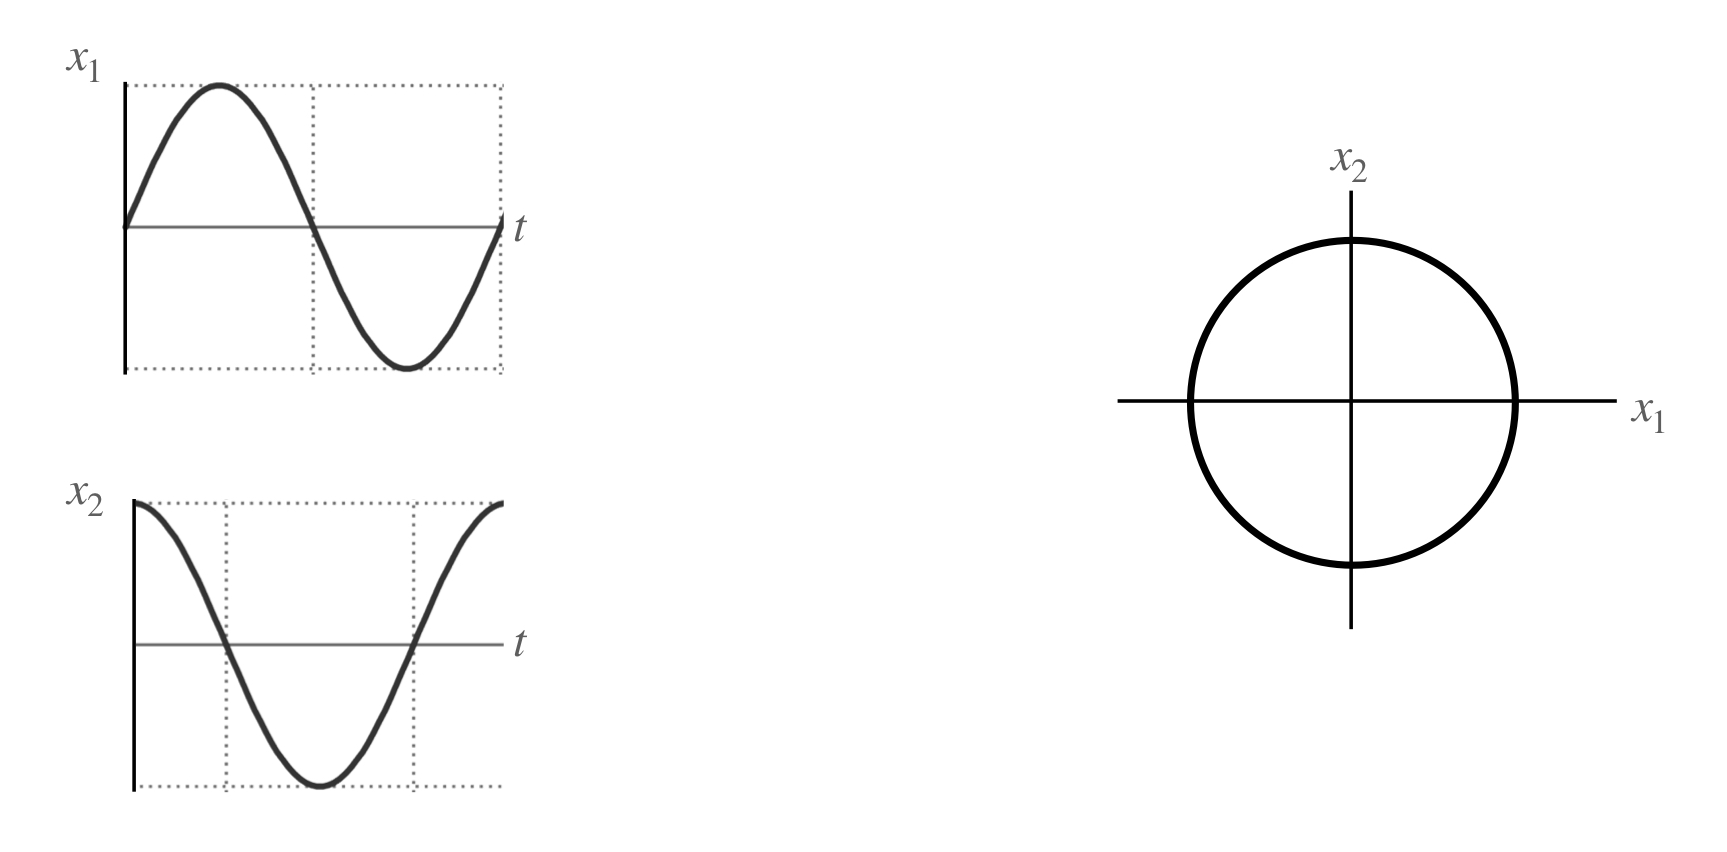
\includegraphics[width=\textwidth]{./Figs/circle_dynamical_system.jpeg}
        \label{fig:dynamical_system}
    \end{subfigure}
    \begin{subfigure}[b]{0.67\textwidth}
        \centering
        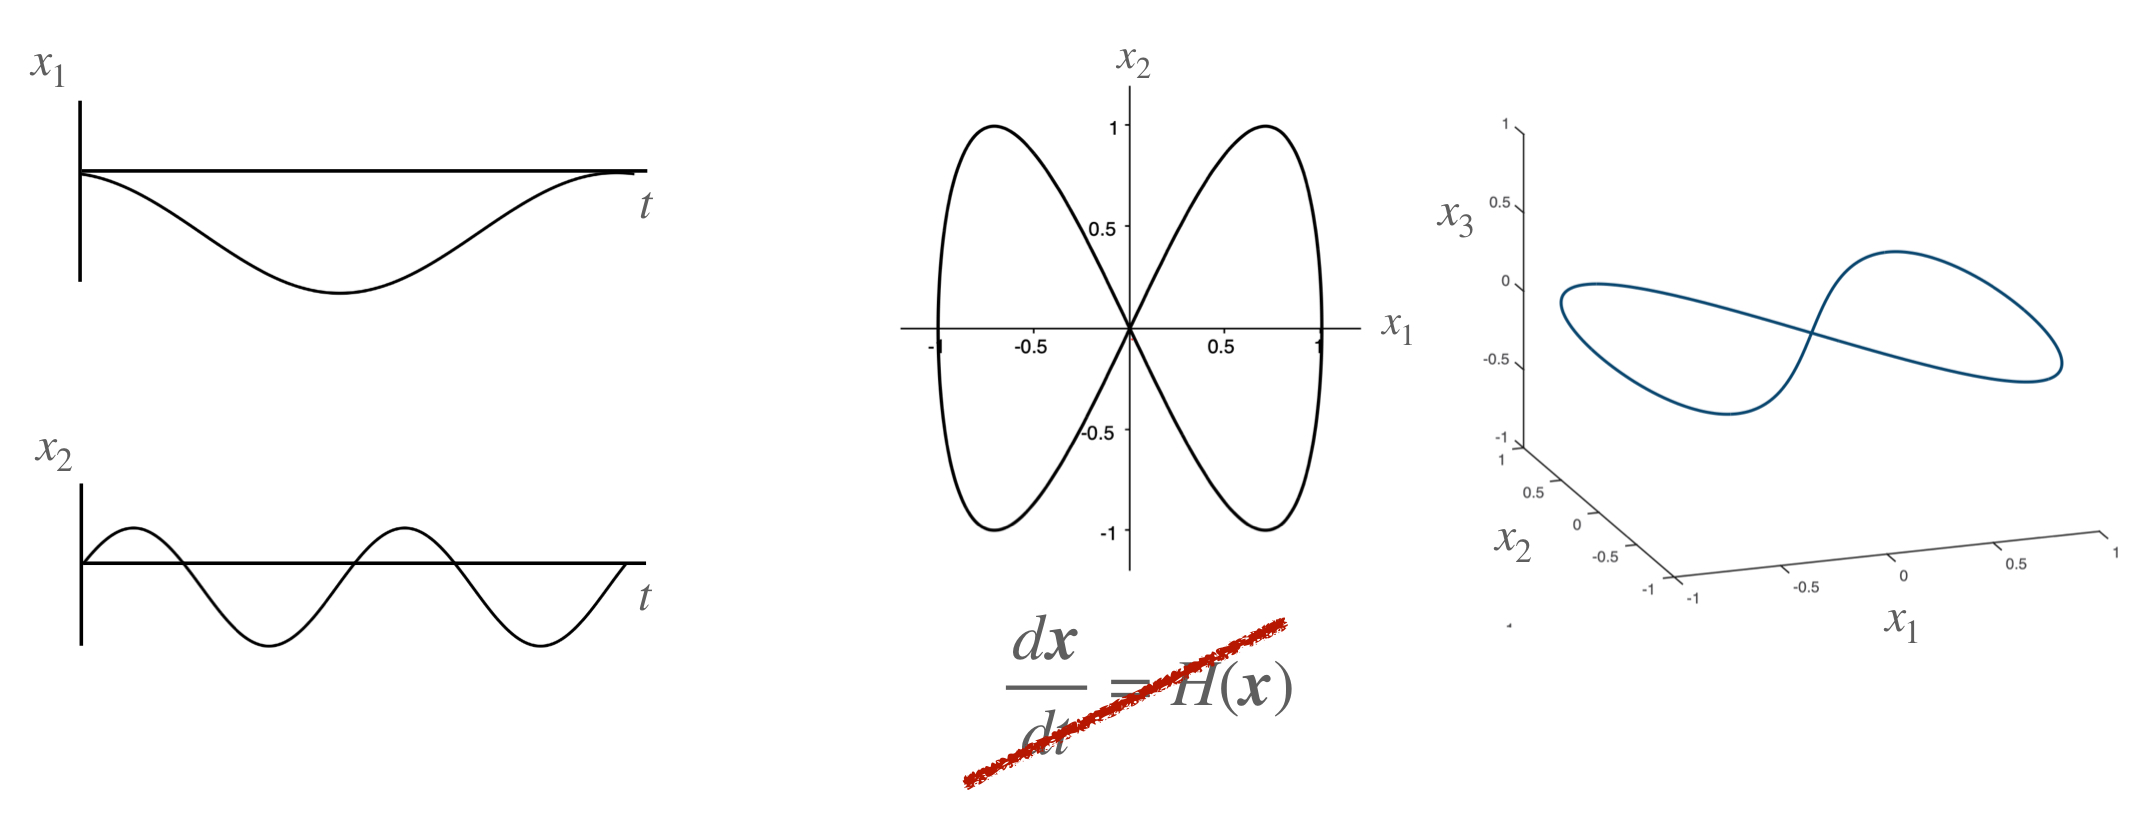
\includegraphics[width=\textwidth]{./Figs/dynamics_2_neurons.jpeg}
        \label{fig:dynamical_system_2_neurons}
    \end{subfigure}
    \caption{Dynamical system of the activity of 2 neurons.}
    \label{fig:dynamical_system}
\end{figure}

\begin{definition}[Measure of entanglement]
    \begin{align}
        Q(t) = \max_{t'} \frac{ \lVert \dot{x_t} - \dot{x_{t'}} \rVert^2 }{ \lVert x_t - x_{t'} + \epsilon \rVert }
    \end{align}
    Where:
    \begin{itemize}
        \item \( x_t \) is the state of the system at time \( t \) (for example, the position of a particle in space)
        \item \( \dot{x_t} \) is the derivative of the state at time \( t \) (for example, the velocity)
        \item \( \epsilon \) is a small constant
    \end{itemize}
    The intuition behind this measure is that if the system is highly entangled, even if the states are close, the derivatives can be very different.
\end{definition}

\begin{definition}[Dynamic system hypothesis]\ \\
    \begin{itemize}
        \item A computation can be described in a low-dimensional state space.
        \item In its basic representation, trajectories may be entangled (not a state space).
        \item By adding some dimensions, we can untangle the trajectory and create a dynamical system landscape.
        \item We want the trajectories to be untangled enough to be robust to noise (Luckily, we have many neurons that can do that).
        \item A recurrent neural network may implement many separate dynamical systems (because they are very high-D). We chose between them using proper initial conditions.
    \end{itemize}    
\end{definition}

\subsection{Motor cortex untangles muscles trajectory}

\subsubsection{Entanglement}
\begin{definition}[Entanglement]\ \\
    A situation where different features or aspects of the data are not clearly separated in the representation space. 
    That means, the learned features are mixed together in such a way that they cannot be easily distinguished or interpreted separately. 
    This can make the model's decisions harder to understand and can affect the model's ability to generalize well to unseen data. 
\end{definition}

\begin{definition}[Untangle]
    The process or the effect of making the learned representations less entangled. 
    This could involve techniques or approaches that aim to separate out the features more distinctly within the model, 
    improving interpretability and possibly the model's performance on certain tasks. 
    It's about making the model's internal representations more structured in a way that different features or aspects of the data are more clearly delineated.
\end{definition}

\begin{definition}[Tangeling]
    The measure of how intertwined the features within a model are
\end{definition}

\begin{definition}[Disentangled]
    The condition where the features or factors of variation in the data are represented in a separated and distinct manner within the model.
\end{definition}

\begin{figure}[h]
    \begin{subfigure}[b]{0.5\textwidth}
        \centering
        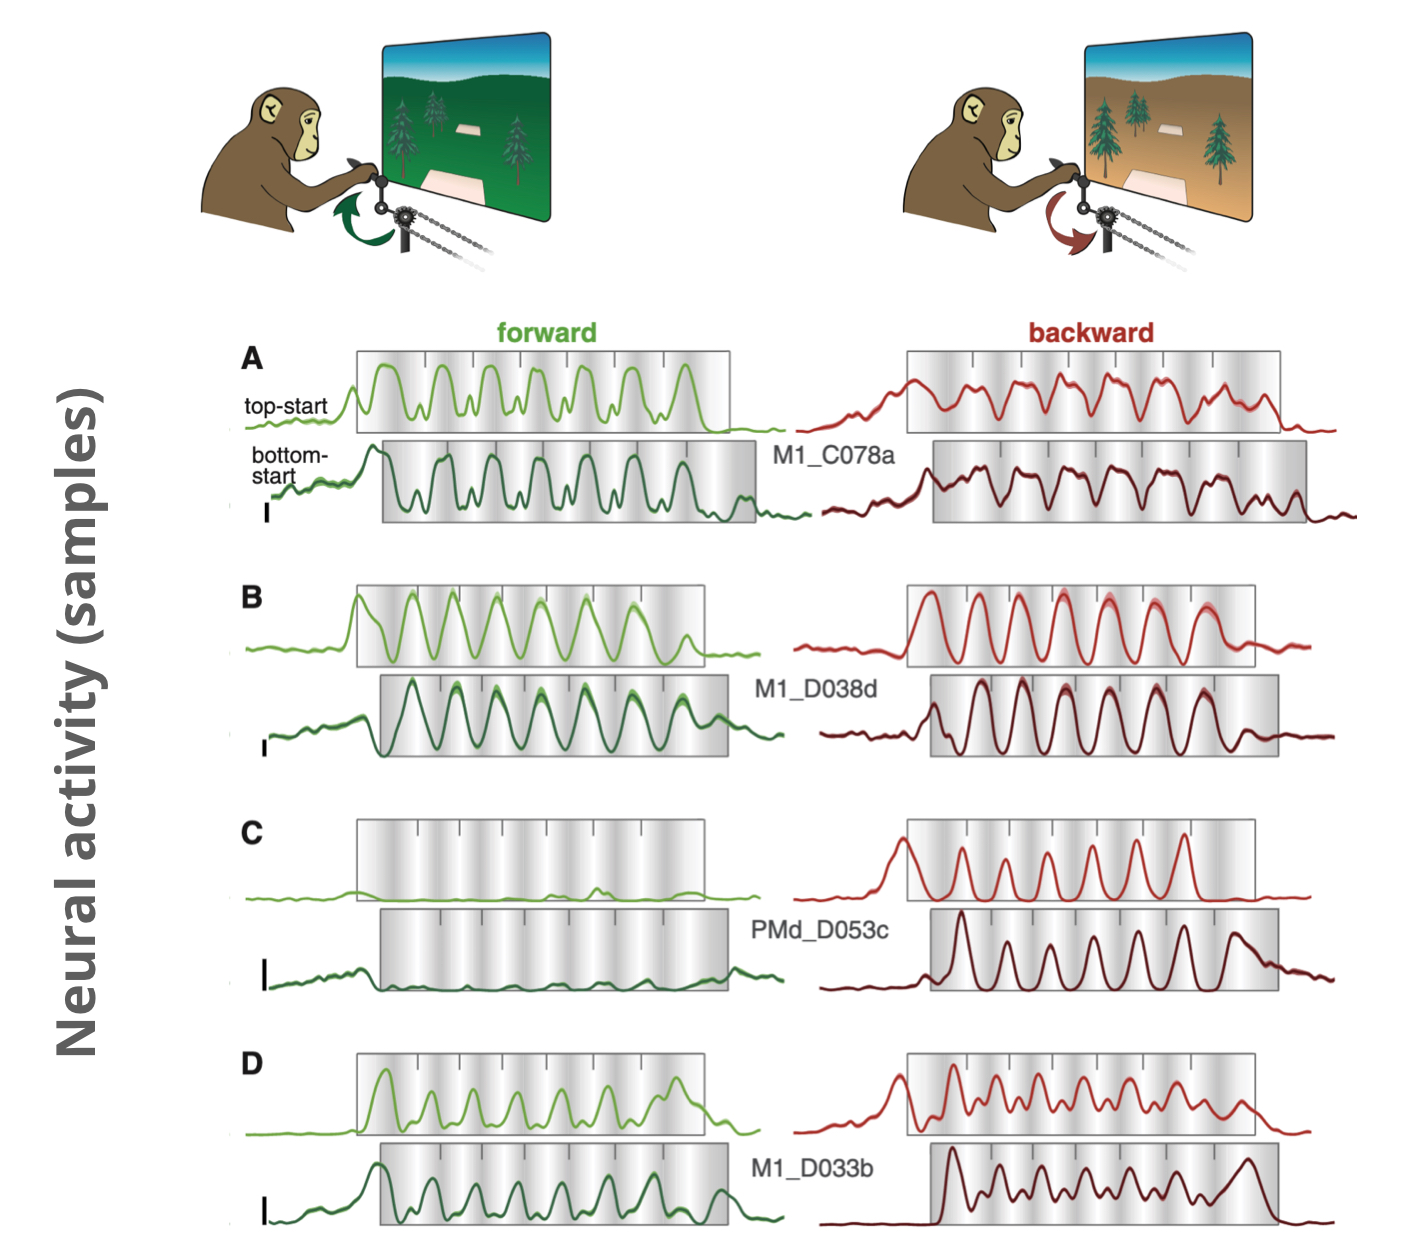
\includegraphics[width=\textwidth]{./Figs/monkey1.jpeg}
        \label{fig:entanglement}
    \end{subfigure}
    \begin{subfigure}[b]{0.5\textwidth}
        \centering
        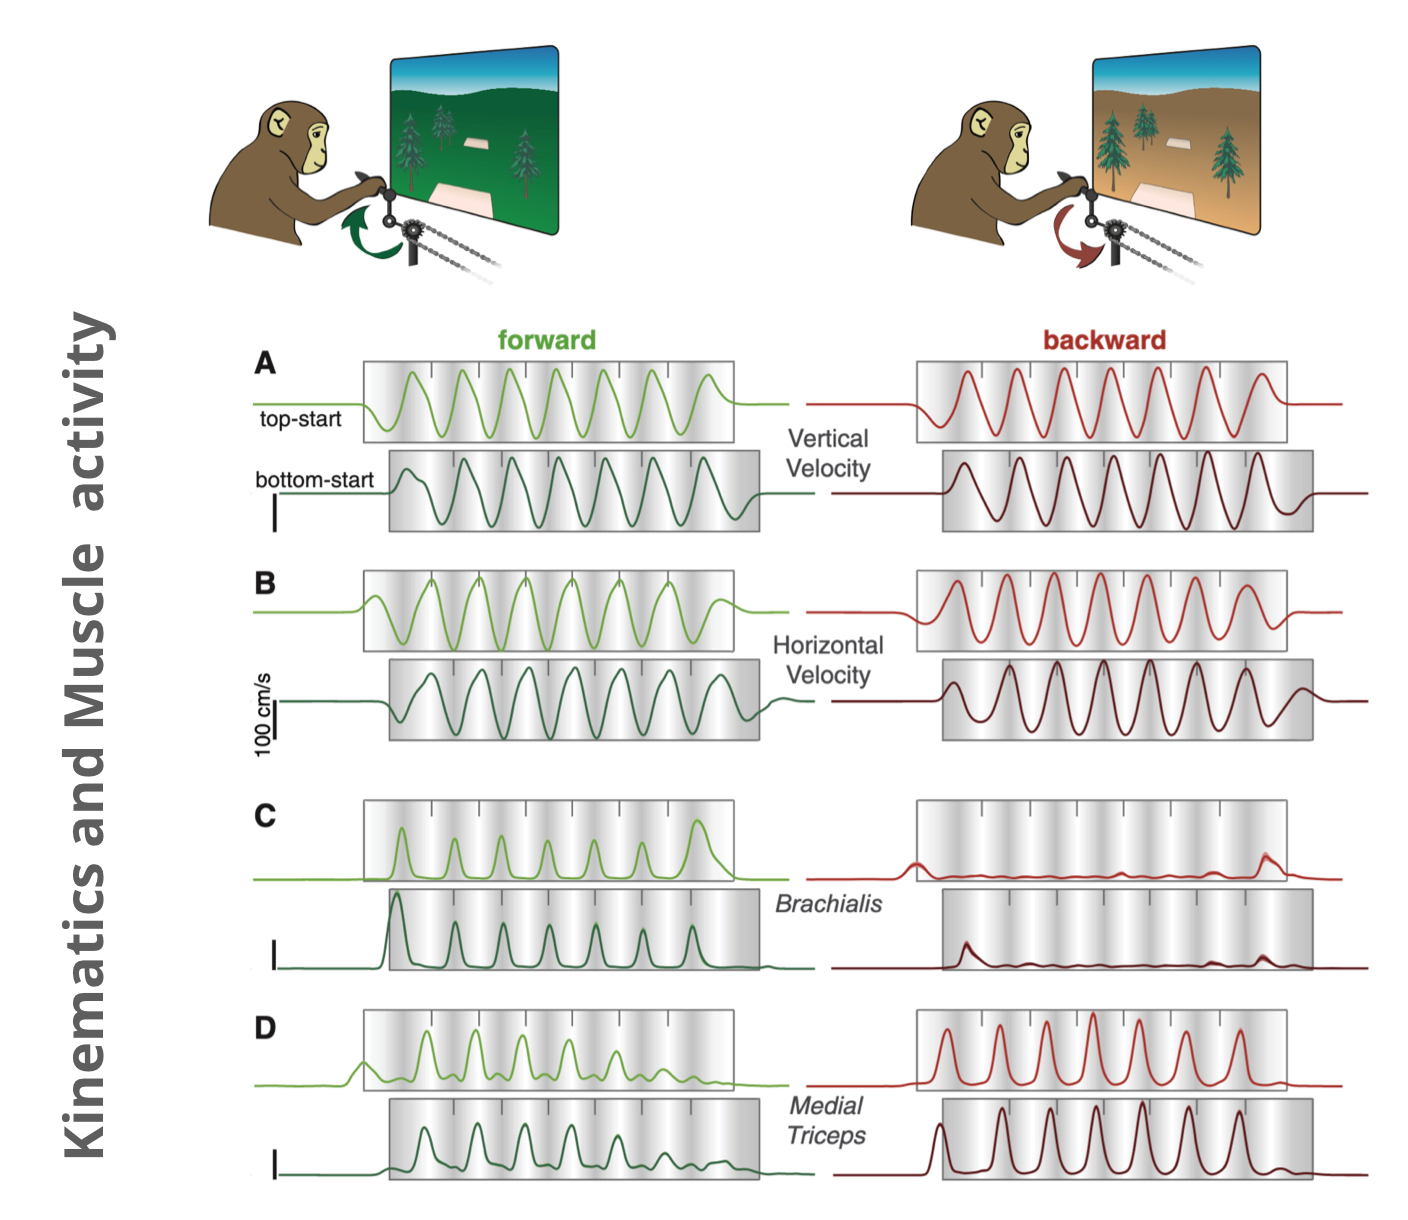
\includegraphics[width=\textwidth]{./Figs/monkey2.jpeg}
        \label{fig:untangling}
    \end{subfigure}
    \caption{Russo et al. (2018) - Entanglement and untangling of muscle trajectories.}
    \label{fig:entanglement_untangling}
\end{figure}


\begin{definition}[EMG (Electromyography)]\ \\
    Electromyography (EMG) is a technique for evaluating and recording the electrical activity produced by skeletal muscles. 
    EMG is performed using an instrument called an electromyograph to produce a record called an electromyogram. 
    An electromyograph detects the electric potential generated by $\textbf{muscle cells when these cells are electrically or neurologically activated}$.
\end{definition}

\begin{figure}[h]
    \centering
    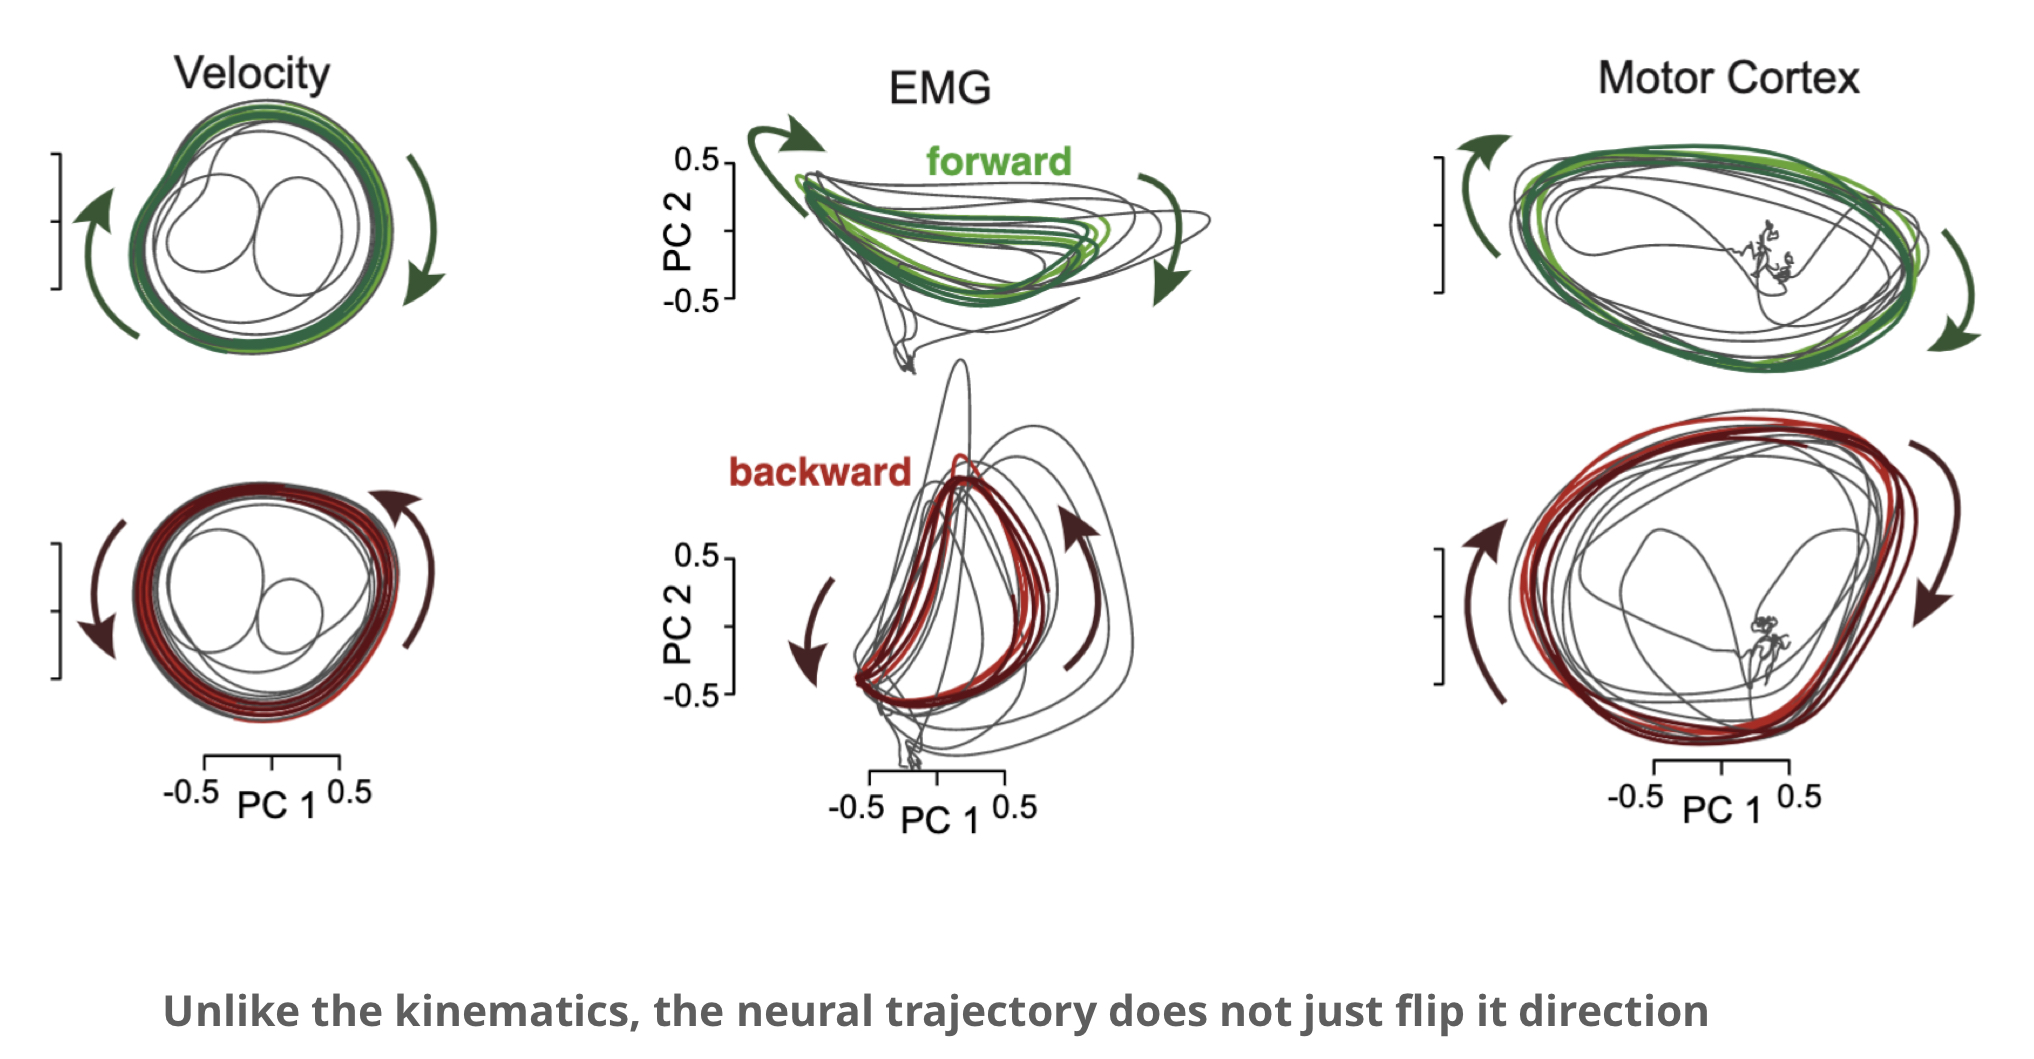
\includegraphics[width=\textwidth]{./Figs/monkey4.jpeg}
    \caption{The first 2 PCs of the velocity, EMG, and motor cortex activity.}
    \label{fig:entanglement_untangling}
\end{figure}

\begin{figure}[h]
    \centering
    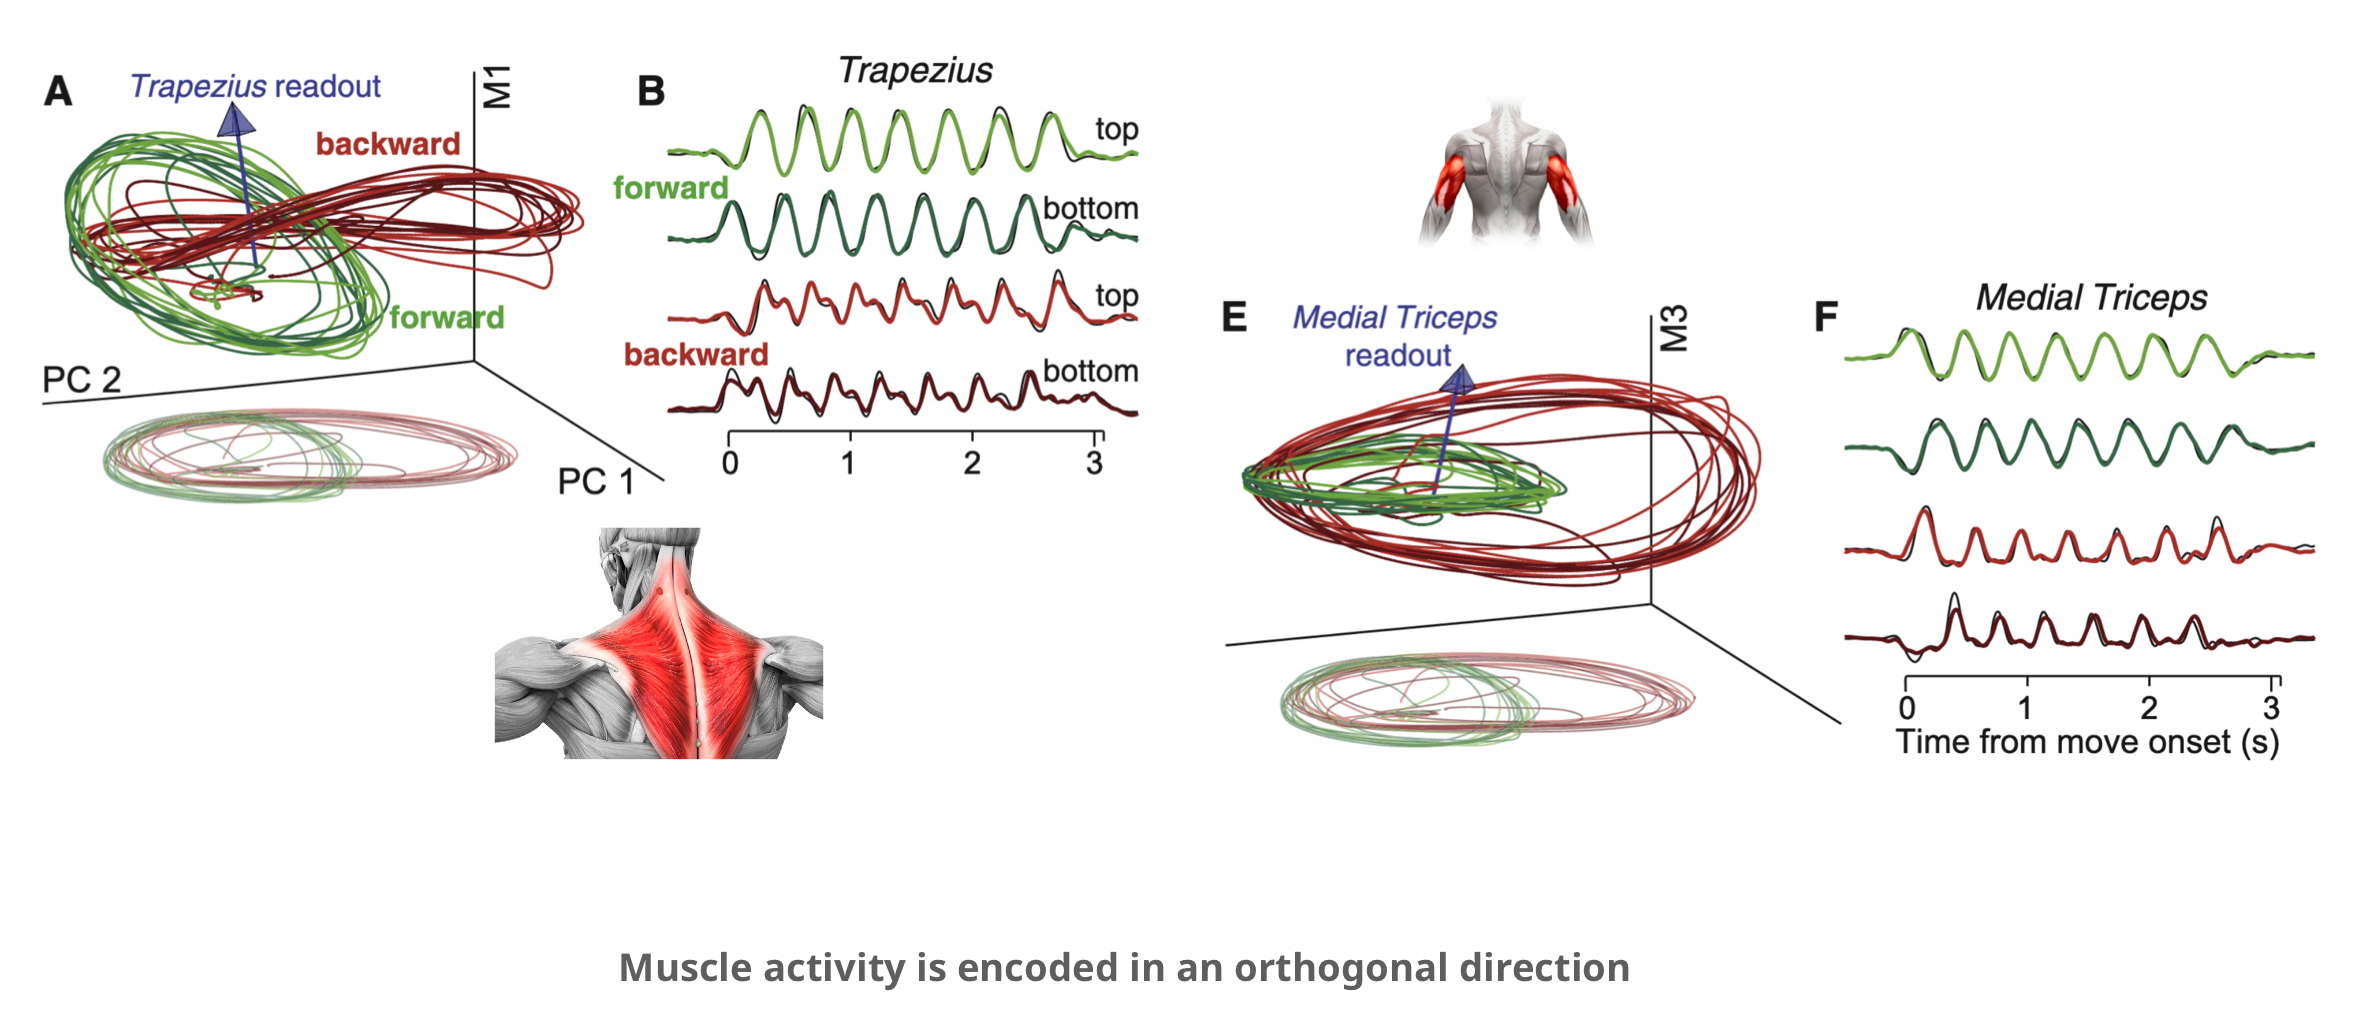
\includegraphics[width=\textwidth]{./Figs/monkey3.jpeg}
    \caption{The trajectories can still be represented as dynamical systems - when we consider higher dimension's representation of the trajectories,
    we can see that the trajectories are disentangled.}    
    \label{fig:entanglement_untangling}
\end{figure}

The researchers wondered if the disentanglement of the trajectories is unique to the motor cortex or if it is a general property of the brain.
The Q parameter on the axis represents the entanglement of the trajectories (Q is the measure of entanglement as shown in the previous section).
They took activities from different areas in the brain (Motor cortex, V1, S1) and checked the entanglement of the nureal activity and EMG trajectories.
The idea of disentanglement is seem to be unique to the motor cortex.

\begin{figure}[h]
    \centering
    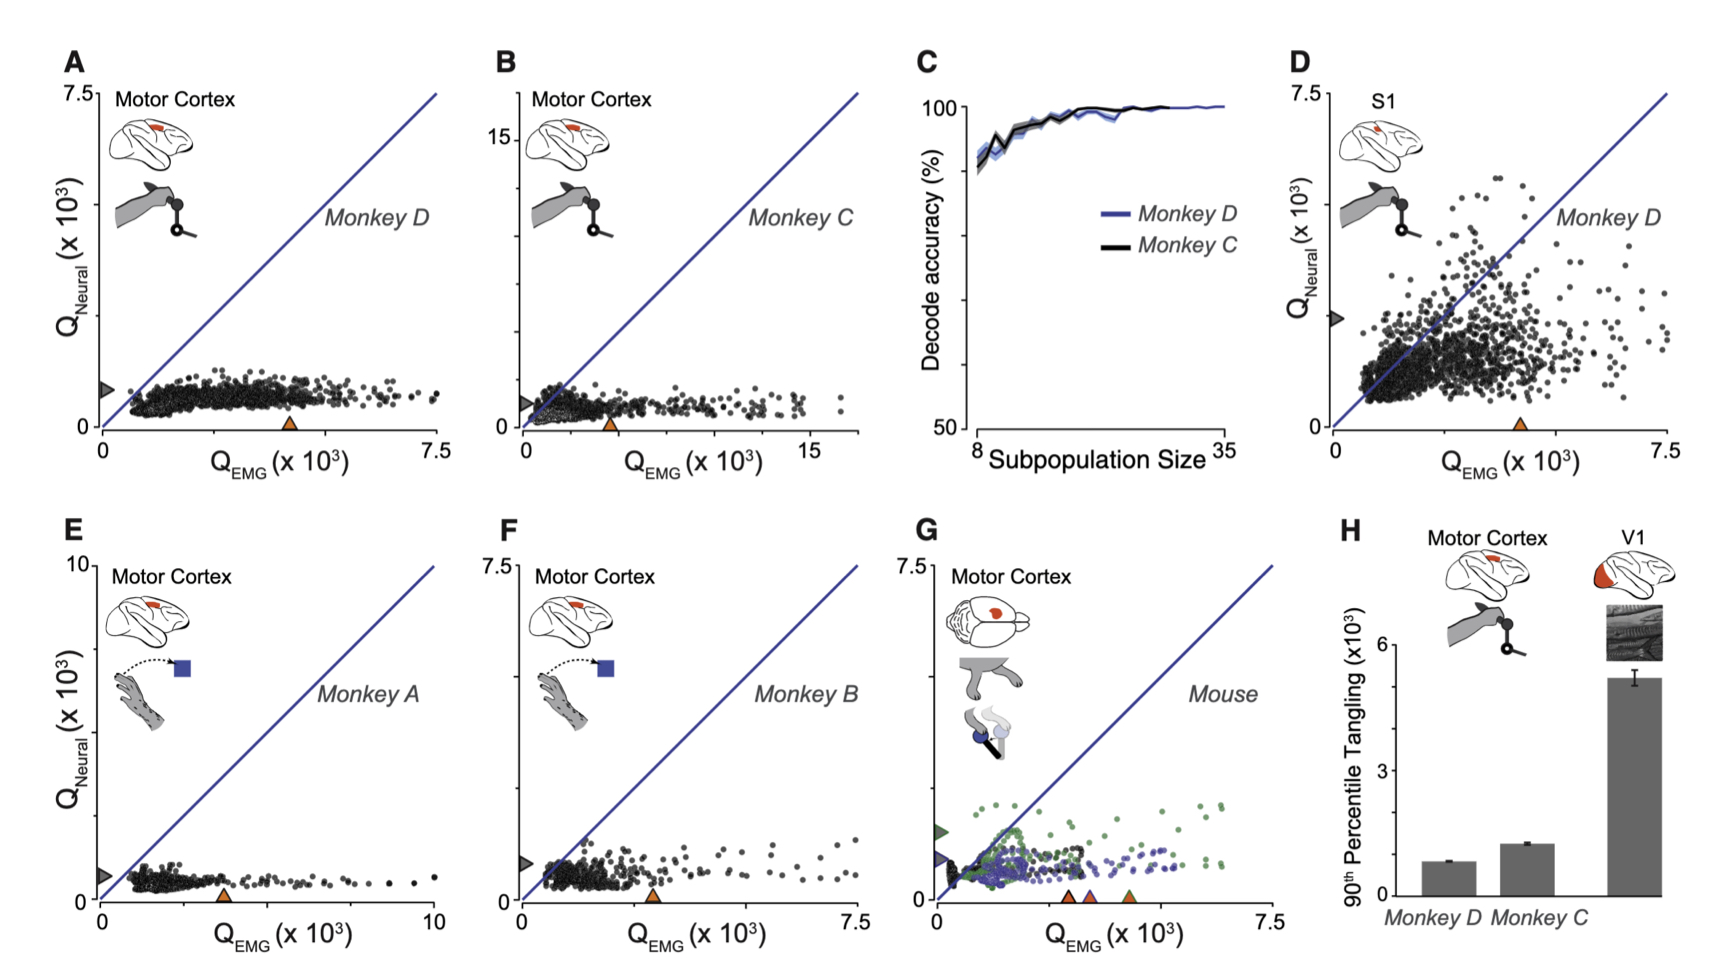
\includegraphics[width=\textwidth]{./Figs/monkey6.jpeg}
    \caption{The activity's trajectory is disentangled in the motor cortex}
    \label{fig:entanglement_untangling}
\end{figure}



\subsection{Neural trajectories in the SMA and Motor Cortex}

The key ideas: 
\begin{itemize}
    \item Tracking of the context is presumably particulary important during temporally extended actions.
    \item The Supplementary Motor Area (SMA) is involved in high-order aspects of motor control: tracking progress throught an action.
    \item Analogous population- trajectory geometry naturally arose in trained networks.
    \item Reveals dynamical and geometrical principles by which neural networks can perform higher-order motor control.
    \item Single neurons do not show the whole picture $\rightarrow$ geometry of population dynamics.
    \item By training NN on an abstraction of the task, the neural mechanisms and dynamics are discovered.
\end{itemize}

\begin{figure}[h]
    \centering
    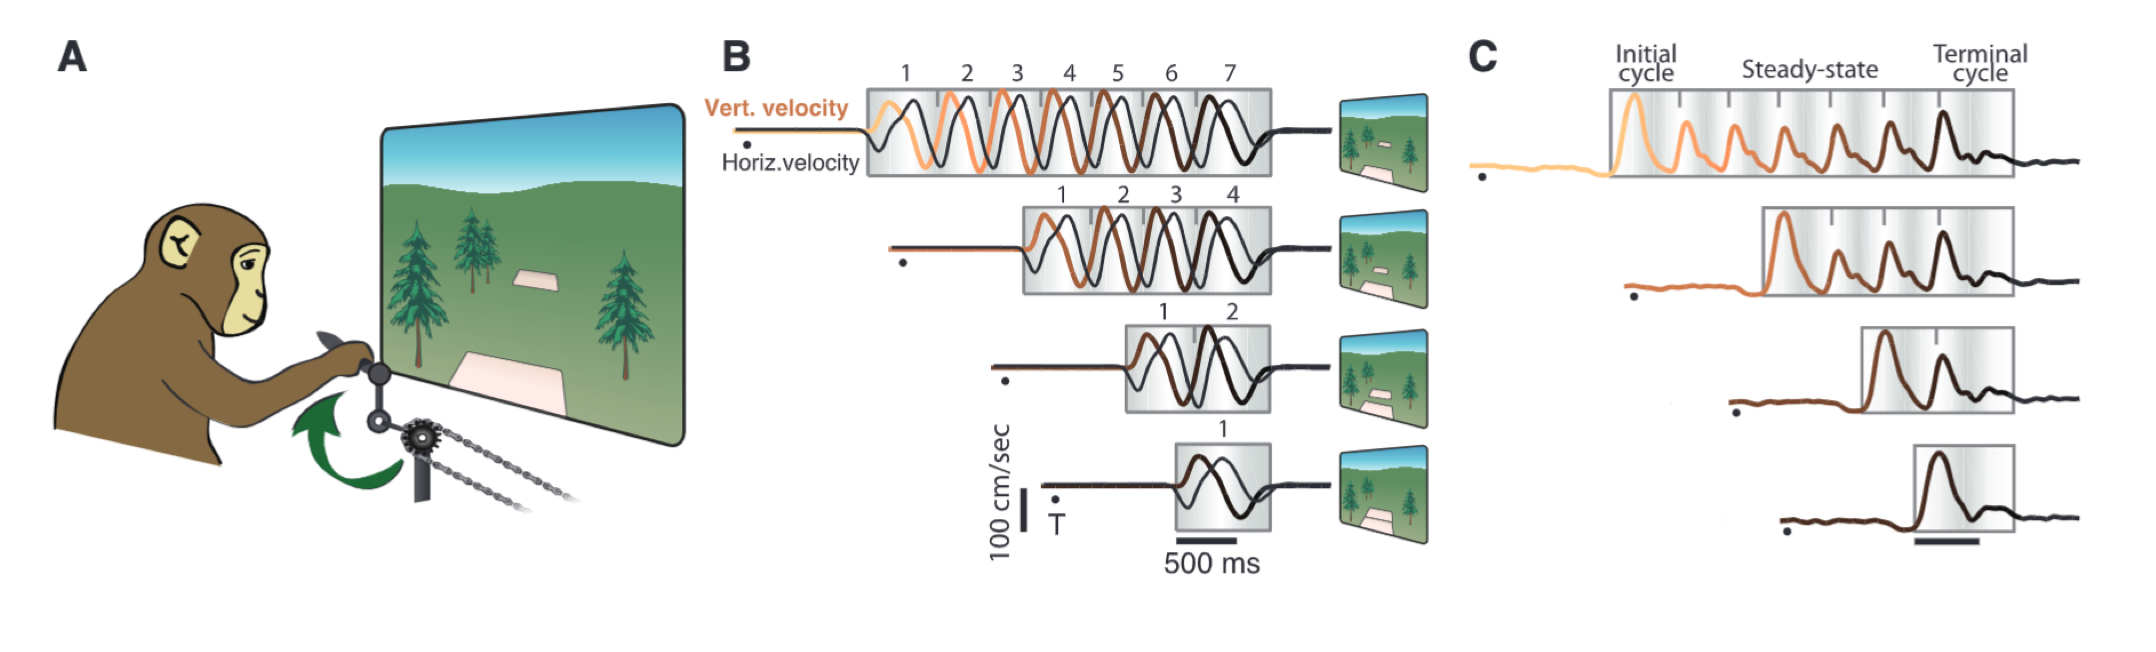
\includegraphics[width=\textwidth]{./Figs/monkeyb1.jpeg}
    \caption{The experiment}
    \label{fig:entanglement_untangling}
\end{figure}

Environment appears (green $\rightarrow$ Forword, desert $\rightarrow$ Backward) in initial position. \\
$\longrightarrow$  every 1000ms, the target appears in the corresponding position to the cycling \\
$\longrightarrow$  the monkey has to reach the target \\



\subsubsection{Supplementary motor area (SMA)}

\begin{figure}[h]
    \centering
    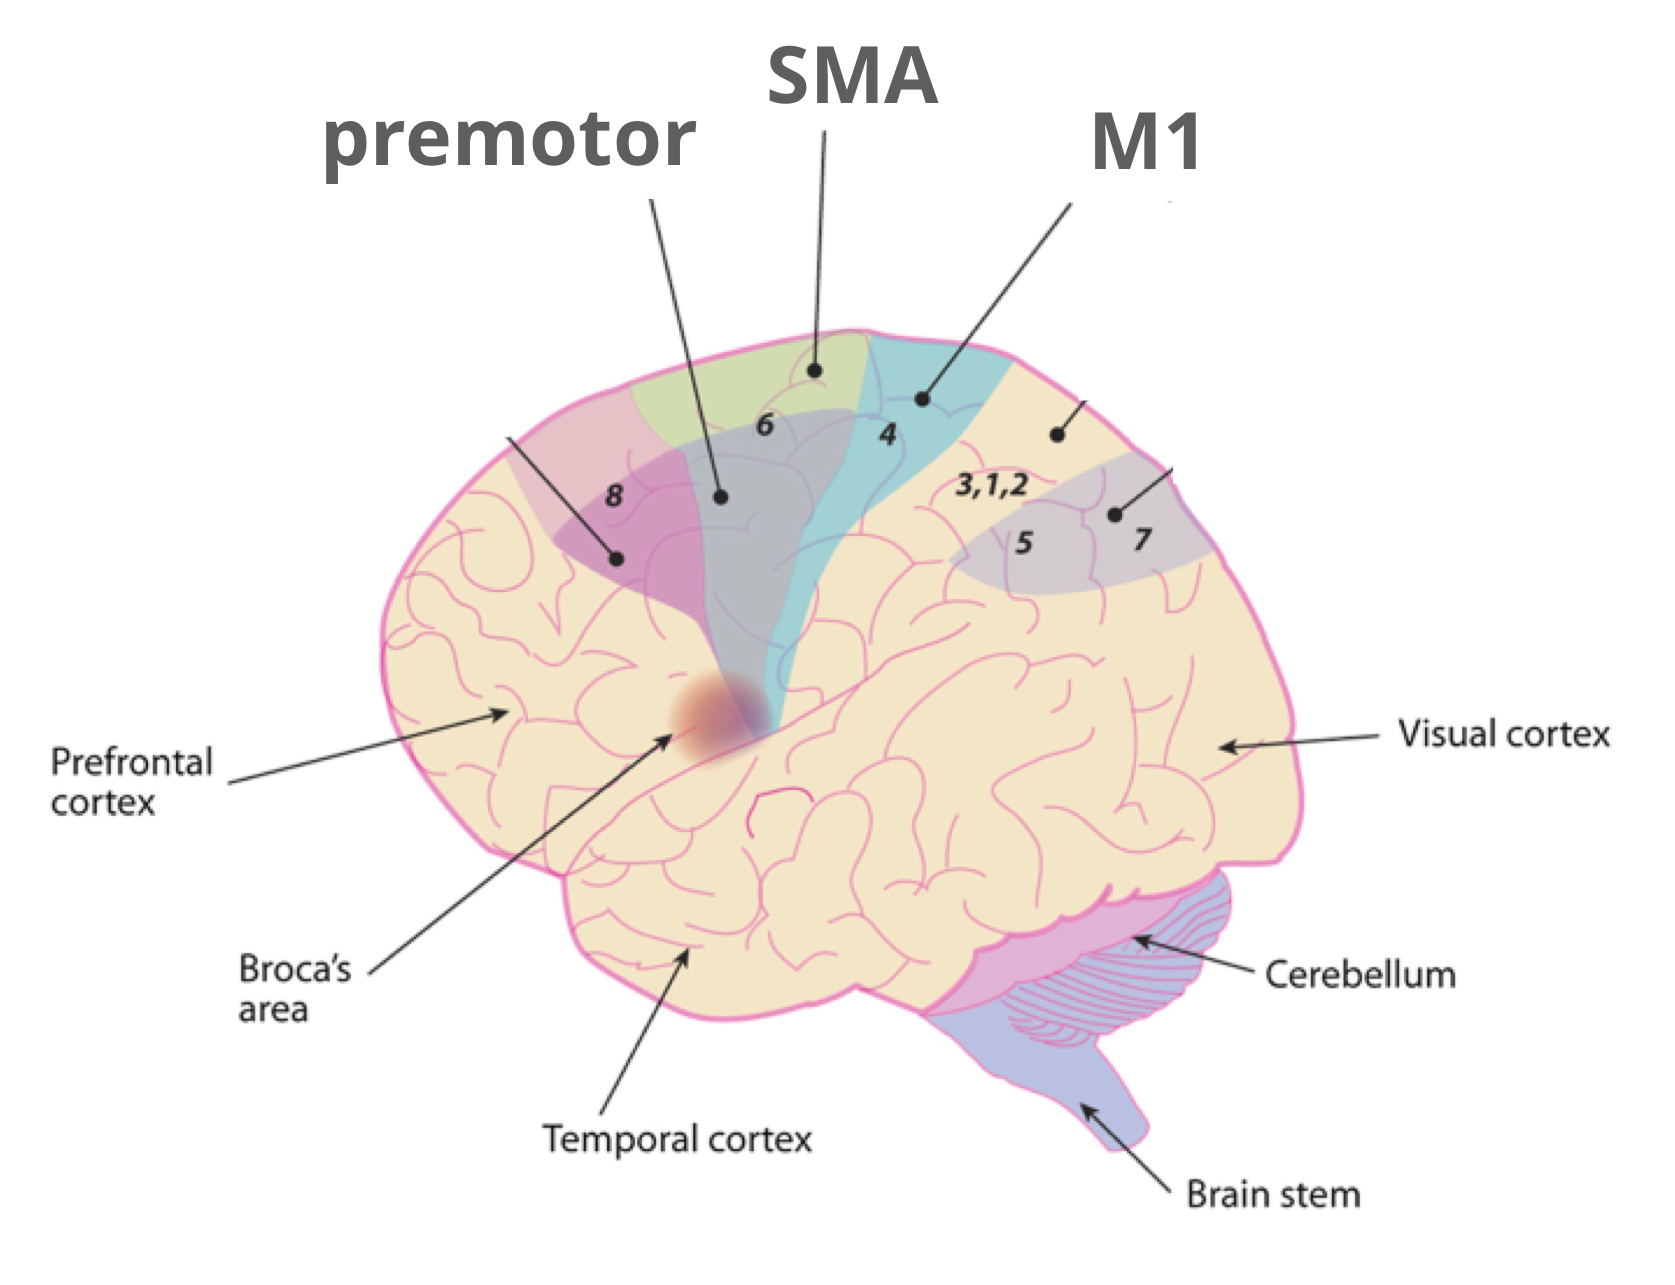
\includegraphics[width=0.6\textwidth]{./Figs/monkey5.jpeg}
    \caption{The motor cortex - M1 (the primary motor cortex), SMA (the supplementary motor area), the permotor cortex, and the prefrontal cortex.}
    \label{fig:entanglement_untangling}
\end{figure}

\begin{itemize}
    \item Part of the motor cortex of primates that contributes to the control of movement.
    \item In monkeys (in hummans similar ideas), the SMA contains a rough map of the body.
    \item Control of internally generated movements and not triggered by sensory events.
    \item Control of sequences of movements.
\end{itemize}

\begin{figure}[h]
    \centering
    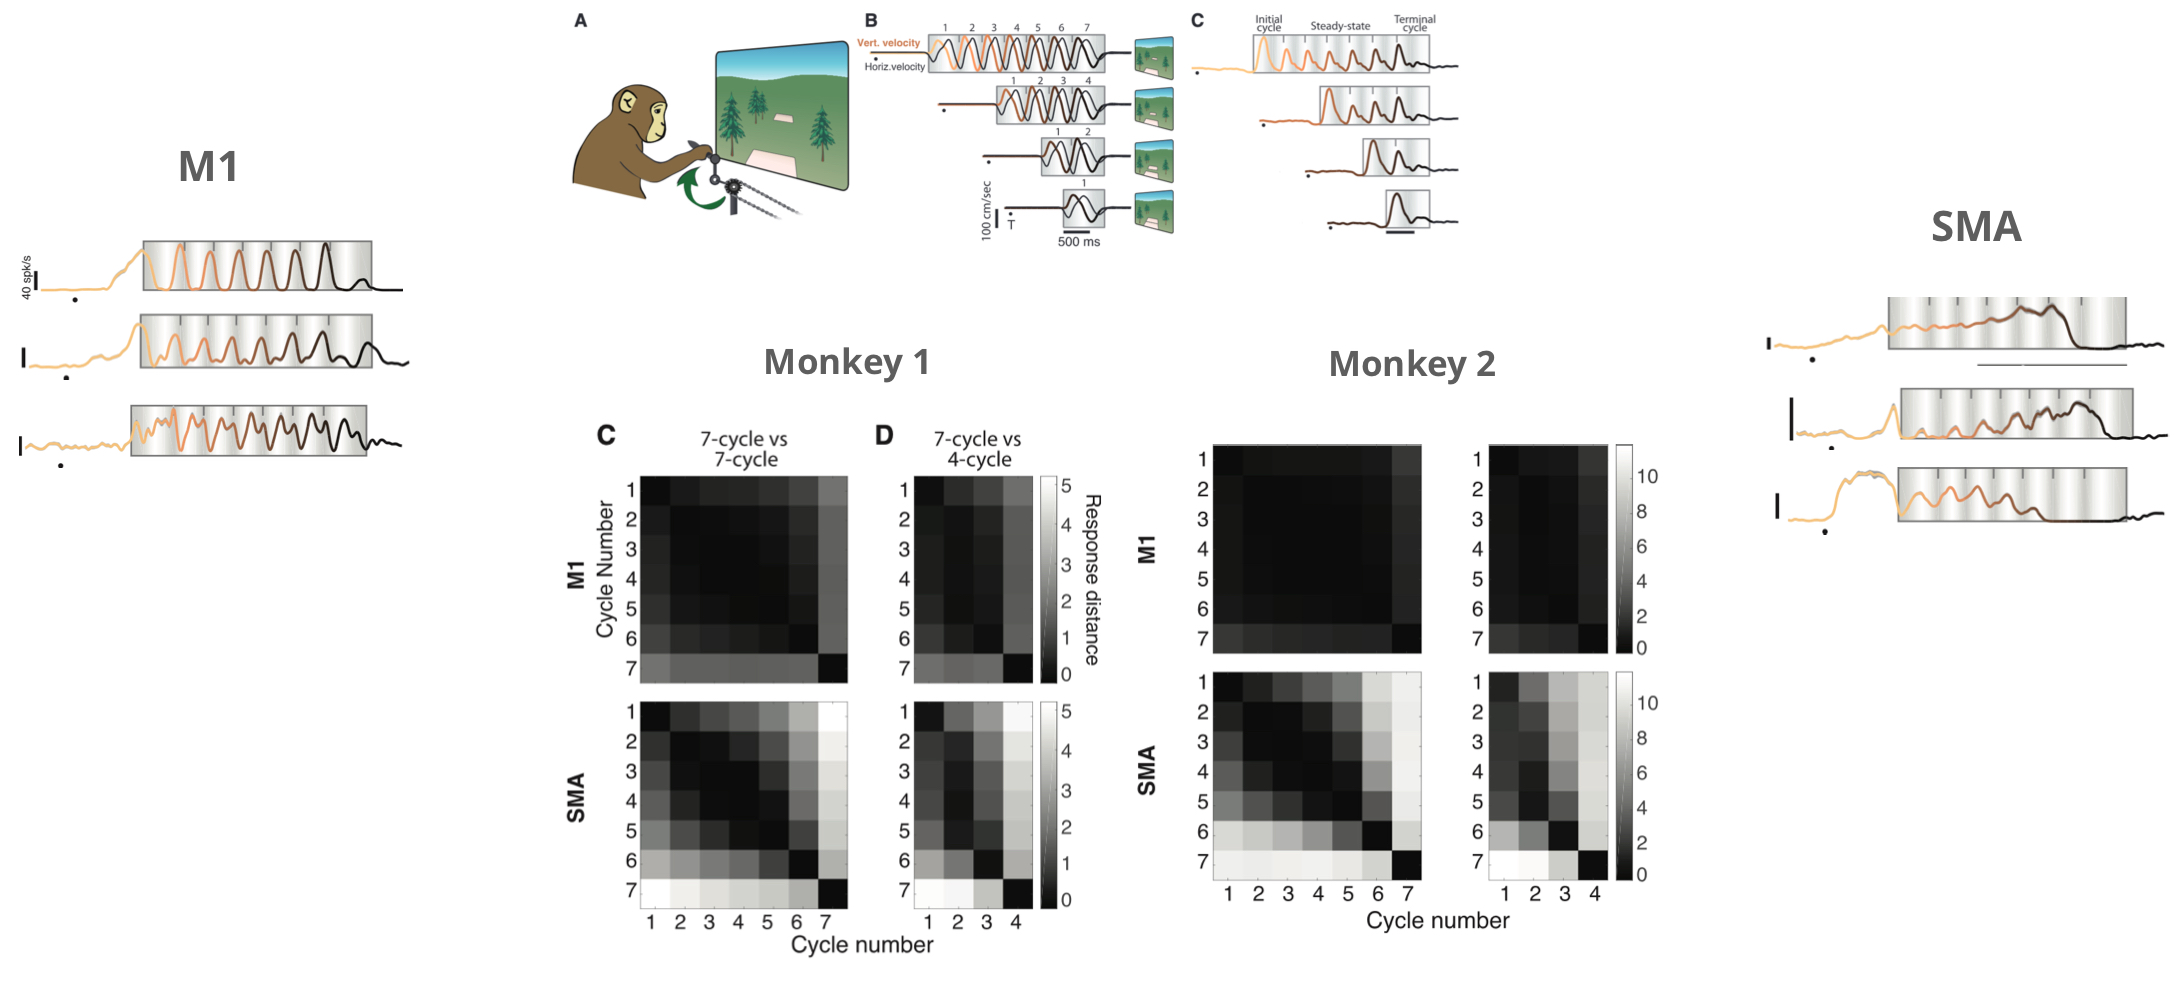
\includegraphics[width=\textwidth]{./Figs/monkeyb2.jpeg}
    \caption{The correlation between different cycles' neural activity in the SMA and M1. In M1 the correlation is high 
    (meaning that the activity is similar in different cycles), while in the SMA the correlation is low (meaning that the activity is different in different cycles).}
    \label{fig:entanglement_untangling}
\end{figure}

The hypothesis - SMA guides movement by tracking contextual factors. 

\begin{figure}[h]
    \centering
    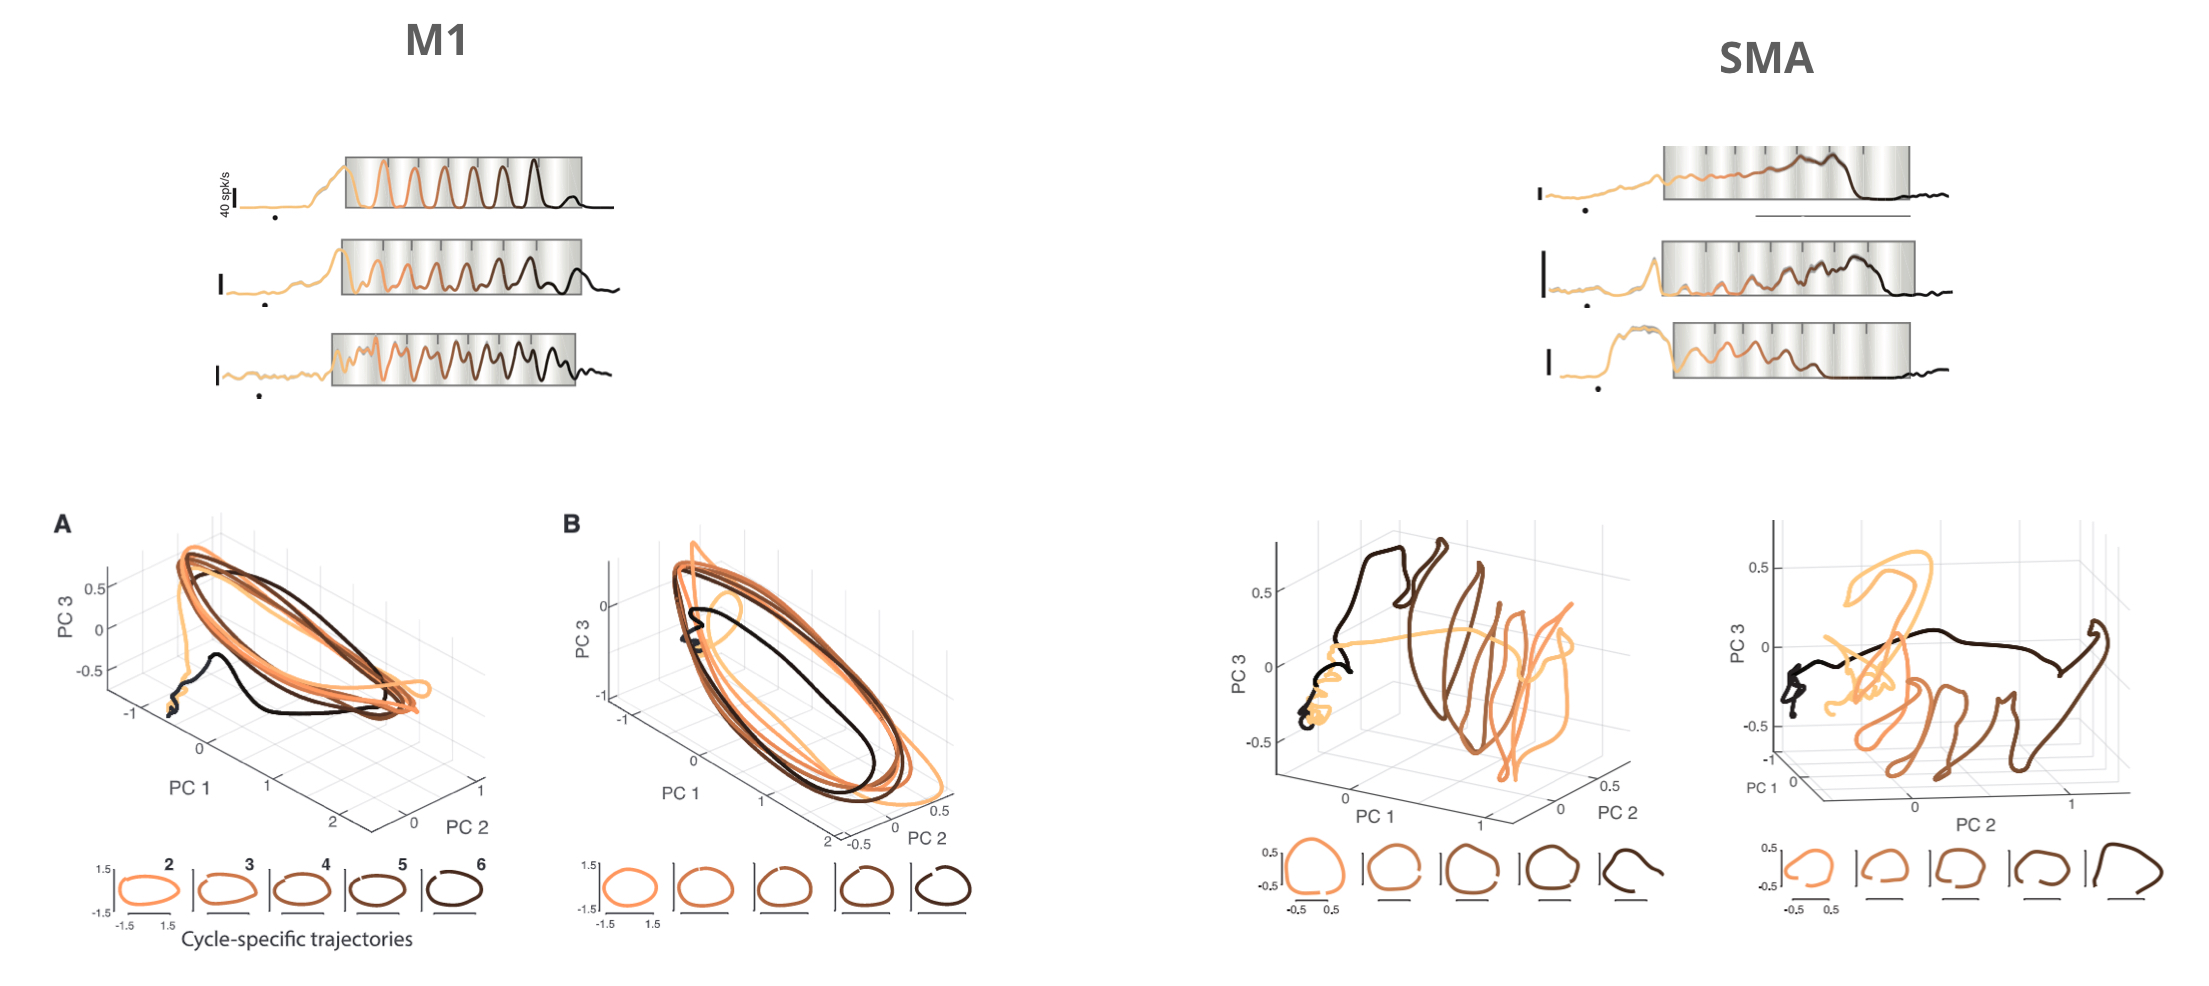
\includegraphics[width=\textwidth]{./Figs/monkeyb3.jpeg}
    \caption{The difference between the PCA of the neural activity in the SMA and M1.}
    \label{fig:entanglement_untangling}
\end{figure}

\textbf{Hypothesis:} A helical SMA population trajectory is a natural solution to the problem of internally tracking motor context during multi-cycle rhythmic movement.

Training RNN to generate the cycles of the experiment. \\
\begin{itemize}
    \item Backpropagation through time
    \item Naive networks: Pulse for initiation and pulse for termination separated by 4-7 cycles
    \item Context tracking: Only input pulse with information about the number of cycles to produce
\end{itemize}
  
\begin{figure}[h]
    \centering
    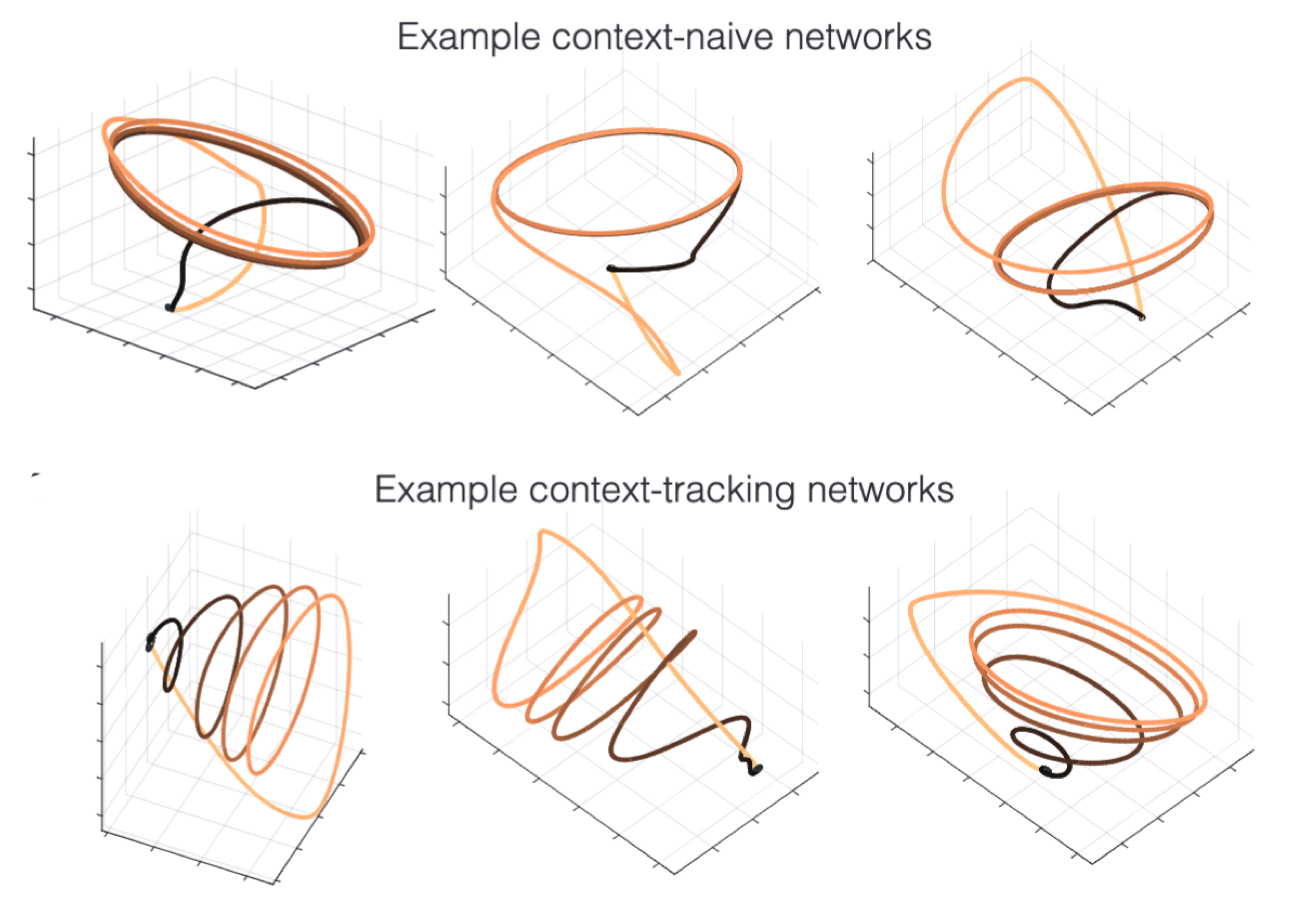
\includegraphics[width=0.5\textwidth]{./Figs/monkeyb4.jpeg}
    \caption{The PCA of the neural activity in the trained network (naive and context tracking).}
    \label{fig:entanglement_untangling}
\end{figure}

Assumptions/Criticisms:
\begin{itemize}
    \item What is the role of visual cues vs internal tracking of motion?
    \item What happens in non-motor areas? Is the prefrontal cortex involved in tracking the context?
    \item Why do we need two different areas? It seems that the SMA has the required information 
    (The answer could be anathomy (M1 really controls the movement) or flexibility (M1 should perform other tasks)).
\end{itemize}


\subsection{Context-dependent computation by recurent dynamics in Prefrontal Cortex (PFC)}

\subsubsection{Key ideas}

\begin{enumerate}
    \item The prefrontal cortex (PFC) performs context-dependent integration.
    \item Individual neurons have very complex activity patterns, and it is hard to understand anything from them.
    \item Study the population dynamics of PFC of macaques performing a context-dependent integration task.
    \item Activity can be understood as part of a dynamical system that controls the population activity.
    \item By training artificial networks, they can reproduce the population dynamics.
    \item Compare data and trained neural networks to different models.
    \item The analysis suggests a new mechanism for context-dependent integration.
\end{enumerate}

\subsubsection{Background}

\begin{itemize}
    \item What is context-dependent integration?
    \begin{itemize}
        \item Ability to gather to process information depending on external/internal state.
        \item Behavior involves top-down modulation from PFC, which is known for representing and maintaining contextual knowledge.
    \end{itemize}
    \item It was believed that the effects of context are already apparent in the sensory input stage (integration), 
    and unnecessary inputs are ignored at that stage (until this paper it was believed that all the things that aren't important for a task are ignored but it showed 
    that even higher areas in the brain receives all the input).
\end{itemize}

\subsubsection{Main findings}

\begin{itemize}
    \item They find no evidence that irrelevant sensory inputs are gated, or filtered out before the integration stage.
    \item The selection is made later in the processing (meaning all information is preserved at first).
    \item The same circuit (in PFC) that performs the integration holds the information relevant to the two contexts.
    \item A recurrent neural network model shows dynamics similar to data and explains the underlying mechanism.
\end{itemize}


\subsubsection{The prefrontal cortex}

The prefrontal cortex (PFC) is a cerebral cortex region located at the front of the brain. 
$\textbf{The PFC}$ is instrumental in higher cognitive functions, such as decision-making, planning, and moderating social behavior. 
It is considered the neural substrate for executive functions, orchestrating thoughts and actions in accordance with internal goals.
Its intricate connectivity with other brain regions supports its role as a coordinator of cognitive processes.

\begin{figure}[h]
    \centering
    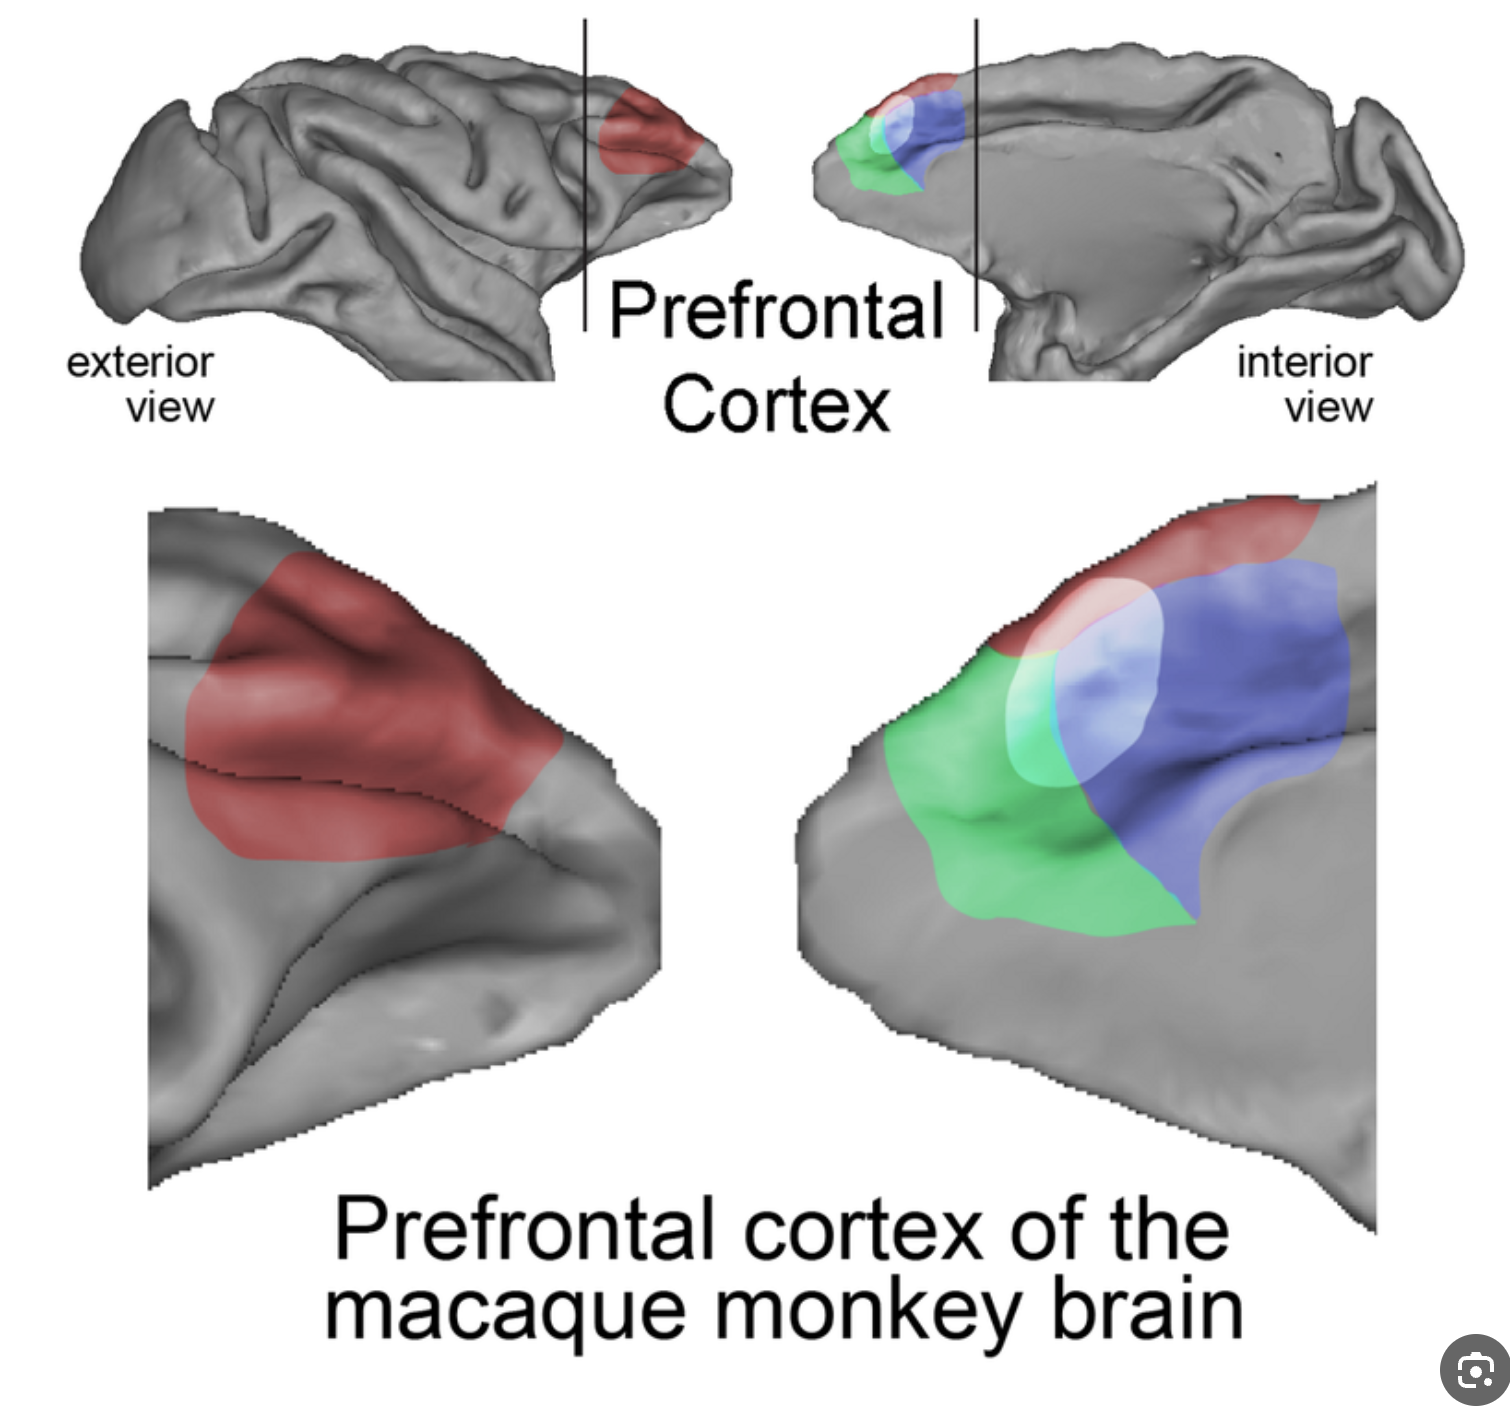
\includegraphics[width=0.3\textwidth]{./Figs/PFC2.png}
    \caption{The prefrontal cortex.}
\end{figure}


\subsubsection{The experiment}


\begin{enumerate}
    \item \textbf{Training and Task}: The monkeys were trained to perform visual discrimination tasks that required them to selectively process and integrate 
    sensory inputs based on the given context. The task required the monkeys to decide based on either the color 
    or the direction of moving dots on a screen, indicated by a contextual cue.

    \item \textbf{Stimuli Presentation}: During the experiments, the monkeys were shown a random-dot motion display where
     they had to discriminate the direction of motion or the color of the dots, depending on the context cue given at the start.

    \item \textbf{Saccadic Responses}: The monkeys had to indicate their decision by making a saccadic eye movement to 
    one of two targets after a delay period. The targets represented the two choices corresponding 
    to the task's context—either motion or color discrimination.

    \item \textbf{Recording Neuronal Activity}: While the monkeys performed these tasks, neuronal activity was recorded from the PFC, 
    specifically around the frontal eye field area, which is known to be involved in saccade planning and execution.

    \item \textbf{Contextual Modulation}: The experiments aimed to understand how irrelevant sensory information is filtered out and 
    how relevant information is enhanced in the PFC during task performance. 
    The hypothesis was that the PFC dynamically selects relevant sensory inputs and integrates them to guide the decision-making process.

    \item \textbf{Data Analysis}: The research involved analyzing the dynamics of neuronal populations in the PFC 
    and developing computational models to understand how neurons in the PFC process different types of information based on context.
    
    \item \textbf{Conclusions}: This study provides insights into the flexible, context-dependent behavior facilitated by the PFC, 
    illustrating that rather than sensory information being pre-filtered, the selection of relevant information occurs within the 
    PFC itself through dynamic processes. The results challenge traditional models of early sensory selection, 
    proposing that selection and integration are aspects of a single dynamical process within the prefrontal circuits.
\end{enumerate}


\begin{figure}[h]
    \centering
    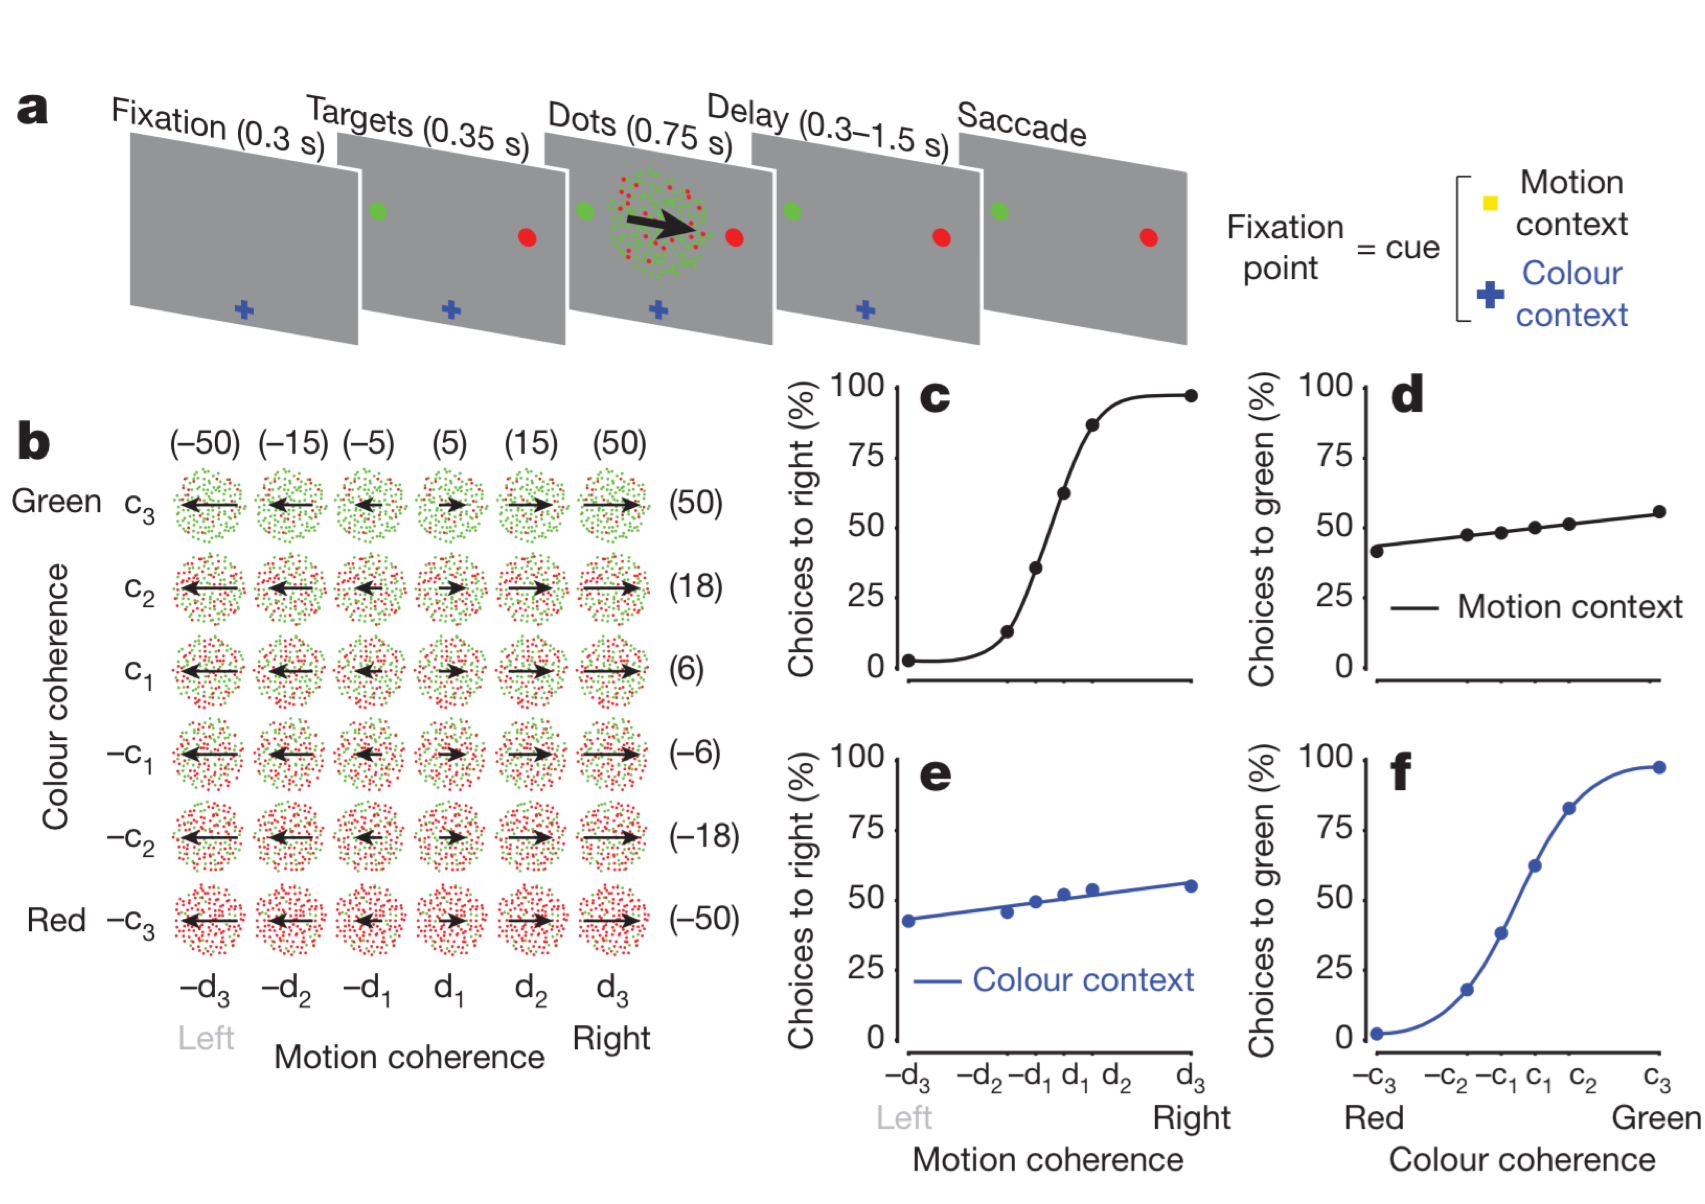
\includegraphics[width=\textwidth]{./Figs/PFC1.jpeg}
    \caption{The experiment task and basic results.}
\end{figure}


\subsubsection{Dynmics of population responses in PFC}

\begin{definition}[Targeted-aligned PCA]
    Targeted-aligned Principal Component Analysis (PCA) is a dimensionality reduction technique applied to neural data to isolate the variance most relevant to the task at hand. 
    In the context of PFC dynamics, this method aligns the axes of the principal components with task-specific variables - such as choice, motion, color, and context. 
\end{definition}


\begin{figure}[h]
    \centering
    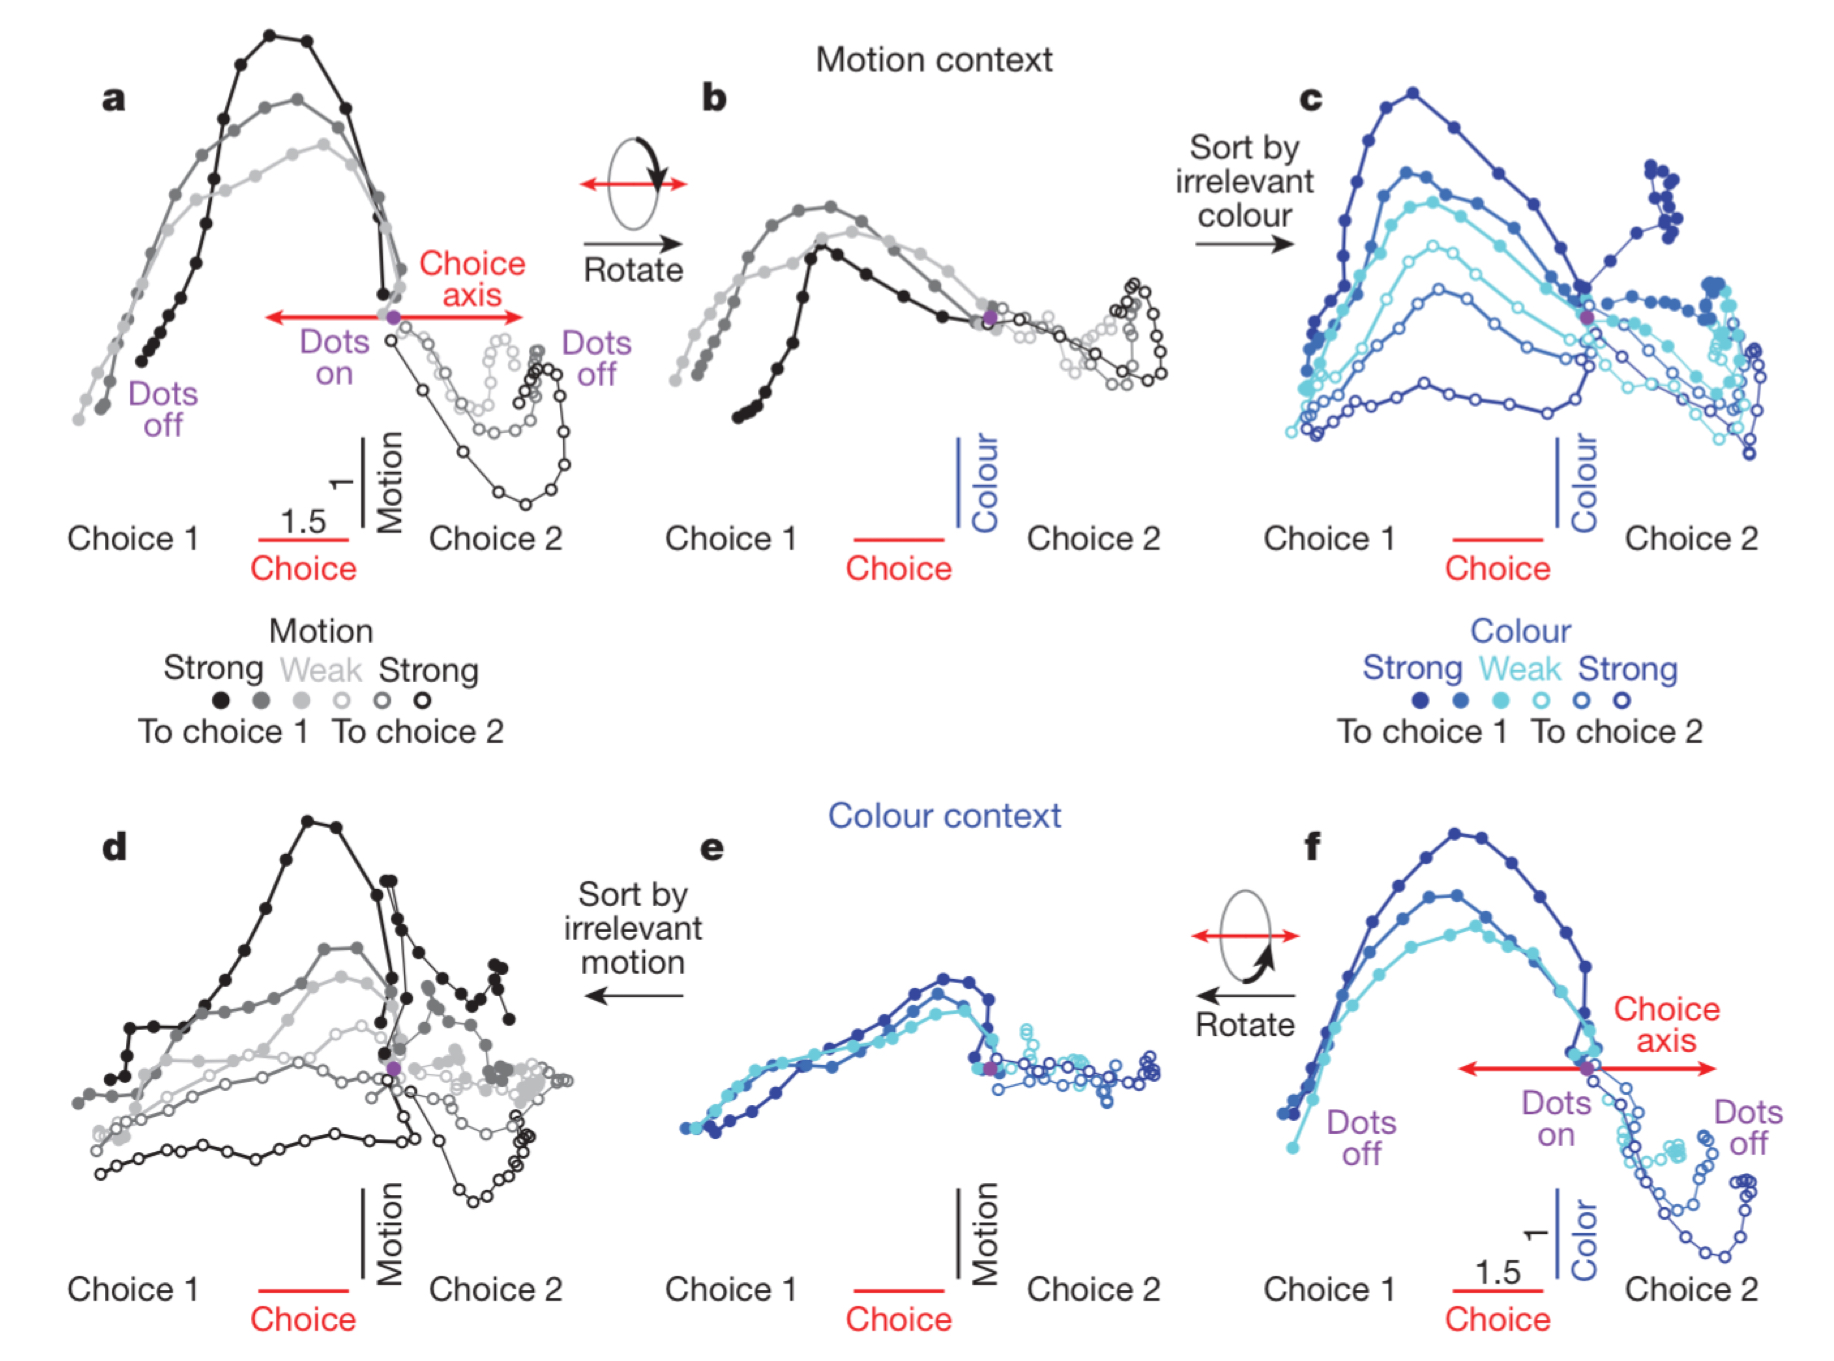
\includegraphics[width=\textwidth]{./Figs/PFC3.jpeg}
    \caption{The dynamics of population responses in the PFC.}
    \label{fig:PFC_PCA}
\end{figure}

What can we infer from the graphs in Figure \ref{fig:PFC_PCA}?
\begin{itemize}
    \item Neural activity does act according as we would expect, but we can see that the entire information is preserved while the decision is made.
    \item Graph c: This shows the sorting of neural responses by irrelevant color in the motion context. 
    Surprisingly, even though color should not influence the choice in the motion context, there's still a distinct separation of neural responses 
    based on the color information. This suggests that the PFC does not entirely filter out irrelevant sensory information before the decision-making stage.
    \item Graph d: This shows the sorting of neural responses by irrelevant motion in the color context.
\end{itemize}

\begin{figure}[h]
    \centering
    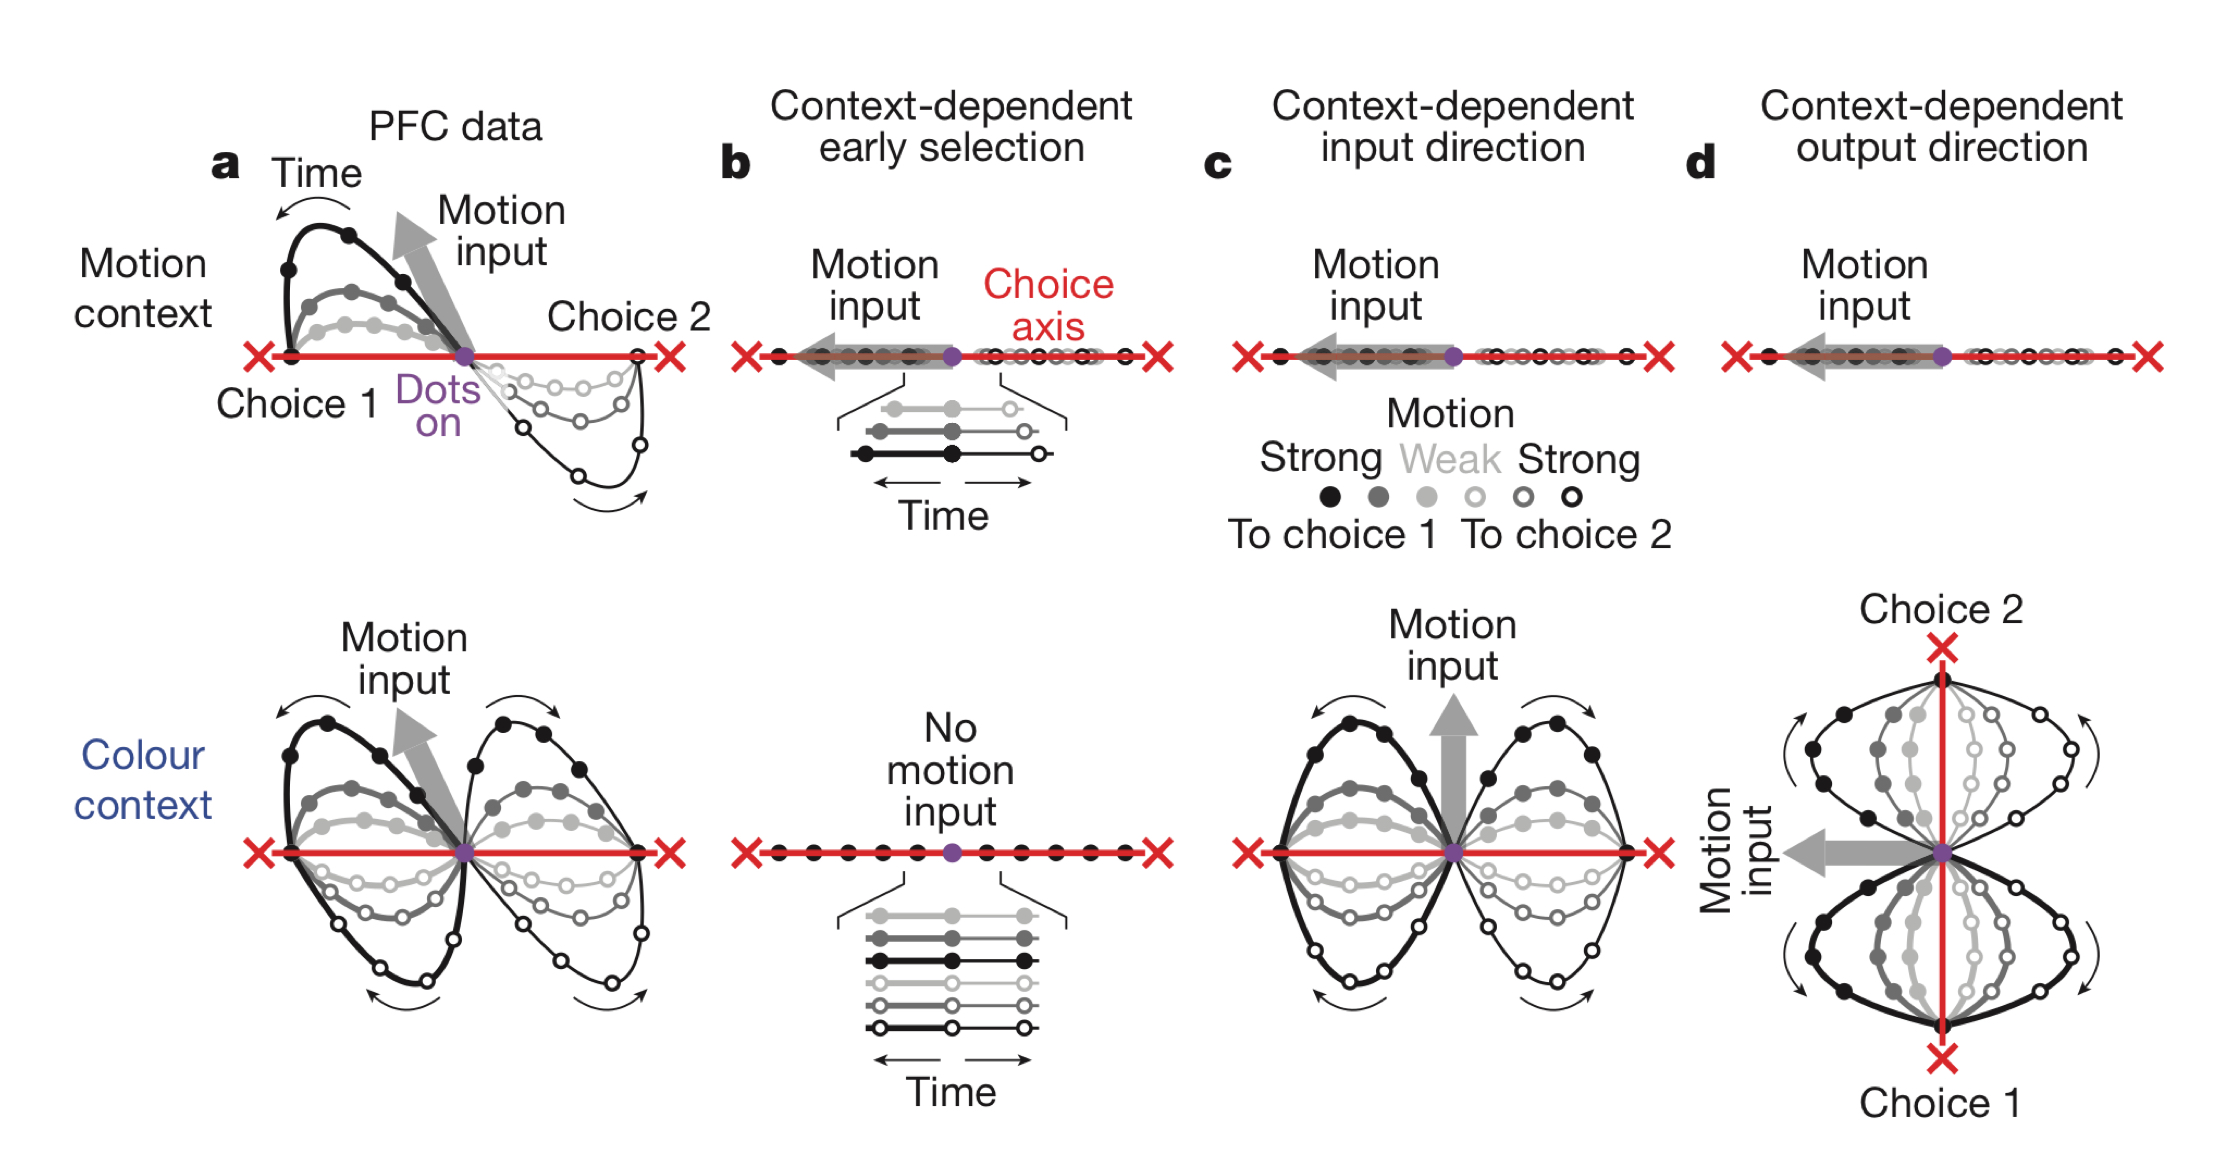
\includegraphics[width=\textwidth]{./Figs/PFC4.jpeg}
    \caption{Models of selective integration inconsistent with PFC responses.}
    \label{fig:PFC_models}
\end{figure}

Figure \ref{fig:PFC_models} illustrates different models of selective integration and compares them to actual PFC (prefrontal cortex) data, 
showcasing how these models are inconsistent with the observed neural responses in the PFC.
\begin{itemize}
    \item $\textbf{Column a - PFC data}$ - where trajectories depict neural activation paths during decision-making in both motion and color contexts.
    The data shows curved trajectories that suggest the PFC processes both relevant and irrelevant sensory information before reaching a decision.
    \item $\textbf{Column b - Context-dependent early selection}$ - posits that the PFC filters out irrelevant sensory information early in the process, 
    allowing only relevant sensory inputs to influence the choice axis. This model is inconsistent with PFC data because the PFC appears 
    to retain and process irrelevant information to some extent, contrary to the filtering-out mechanism suggested by this model.
    \item $\textbf{Column c - Context-dependent input direction}$ - suggests that the relevance of sensory input is determined by its 
    alignment with a choice axis that remains stable across contexts.
    The neural responses are expected to directly align with the choice axis when inputs are relevant. 
    This model is inconsistent with PFC data because the neural trajectories in the PFC do not realign with the choice axis in different contexts—irrelevant inputs still cause deviations.
    \item $\textbf{Column d - Context-dependent output direction}$ - proposes that the choice axis itself shifts depending on the context, aligning with the relevant sensory 
    input to guide decision-making. This too does not align with the PFC data, as the actual neural trajectories do not show a shift 
    in the choice axis with different contexts; instead, both relevant and irrelevant inputs influence trajectories, demonstrating a more complex 
    interaction than a simple shift in the choice axis.
\end{itemize}




They trained a recurrent neural network to perform the task. 
The network was trained to generate the correct saccade based on the context cue (and by that they wanted to get a deeper understanding of the neural activity in the PFC).

\begin{figure}[h]
    \centering
    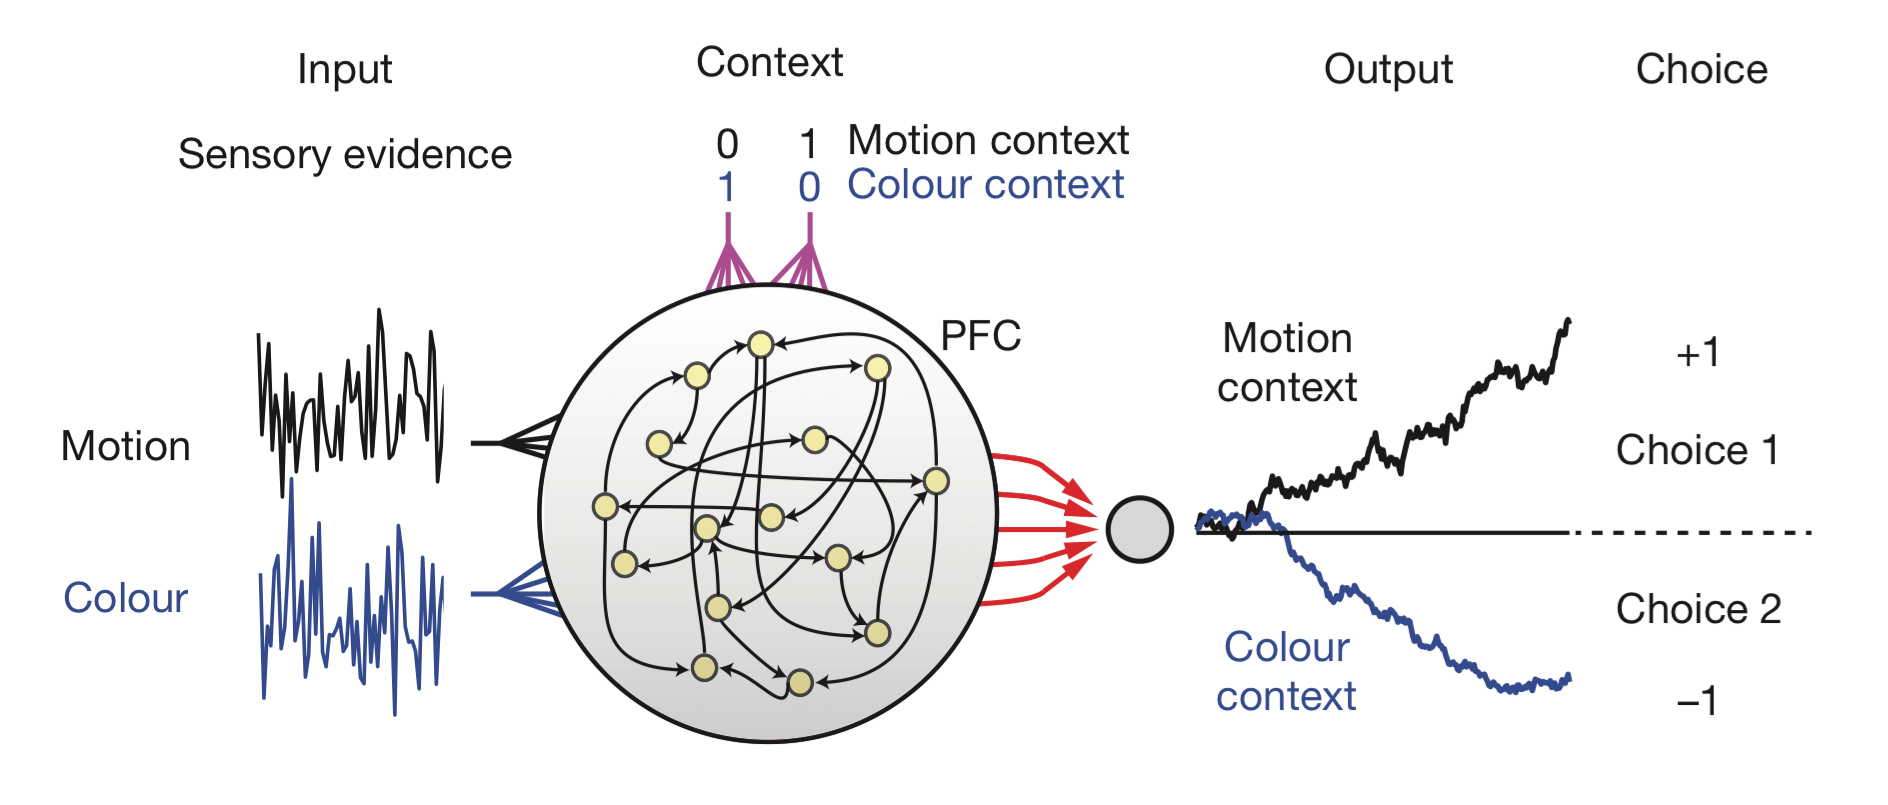
\includegraphics[width=0.8\textwidth]{./Figs/PFC5.jpeg}
    \caption{Artifical neural network model.}
    \label{fig:PFC_NN}
\end{figure}

\begin{figure}[h]
    \centering
    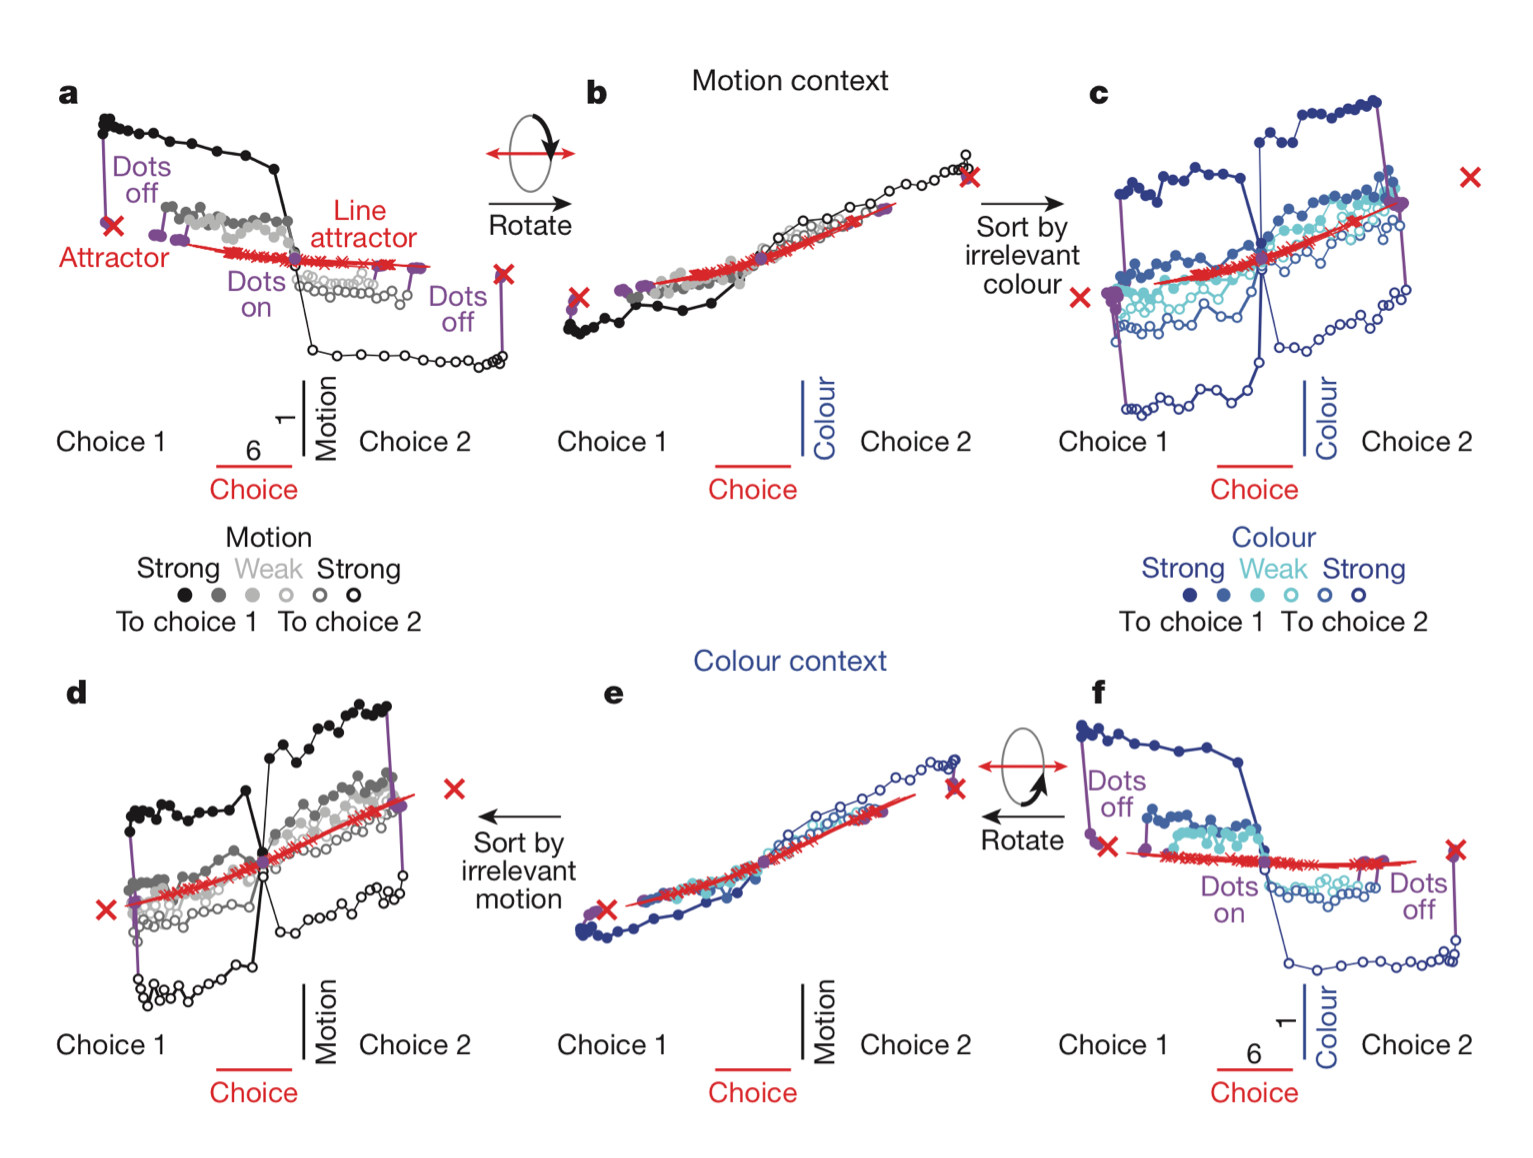
\includegraphics[width=0.8\textwidth]{./Figs/PFC6.jpeg}
    \caption{The PCA of the neural activity in the trained network gave similar results to the data from the PFC.}
    \label{fig:PFC_NN_results}
\end{figure}

\begin{definition}[Line attractor]
    A line attractor is a type of neural network architecture where the neural activity forms a stable trajectory along a line in the state space. 
    This line represents a continuum of possible states or representations, and the neural activity moves along this line to encode different information or states.     
\end{definition}

\begin{figure}[h]
    \centering
    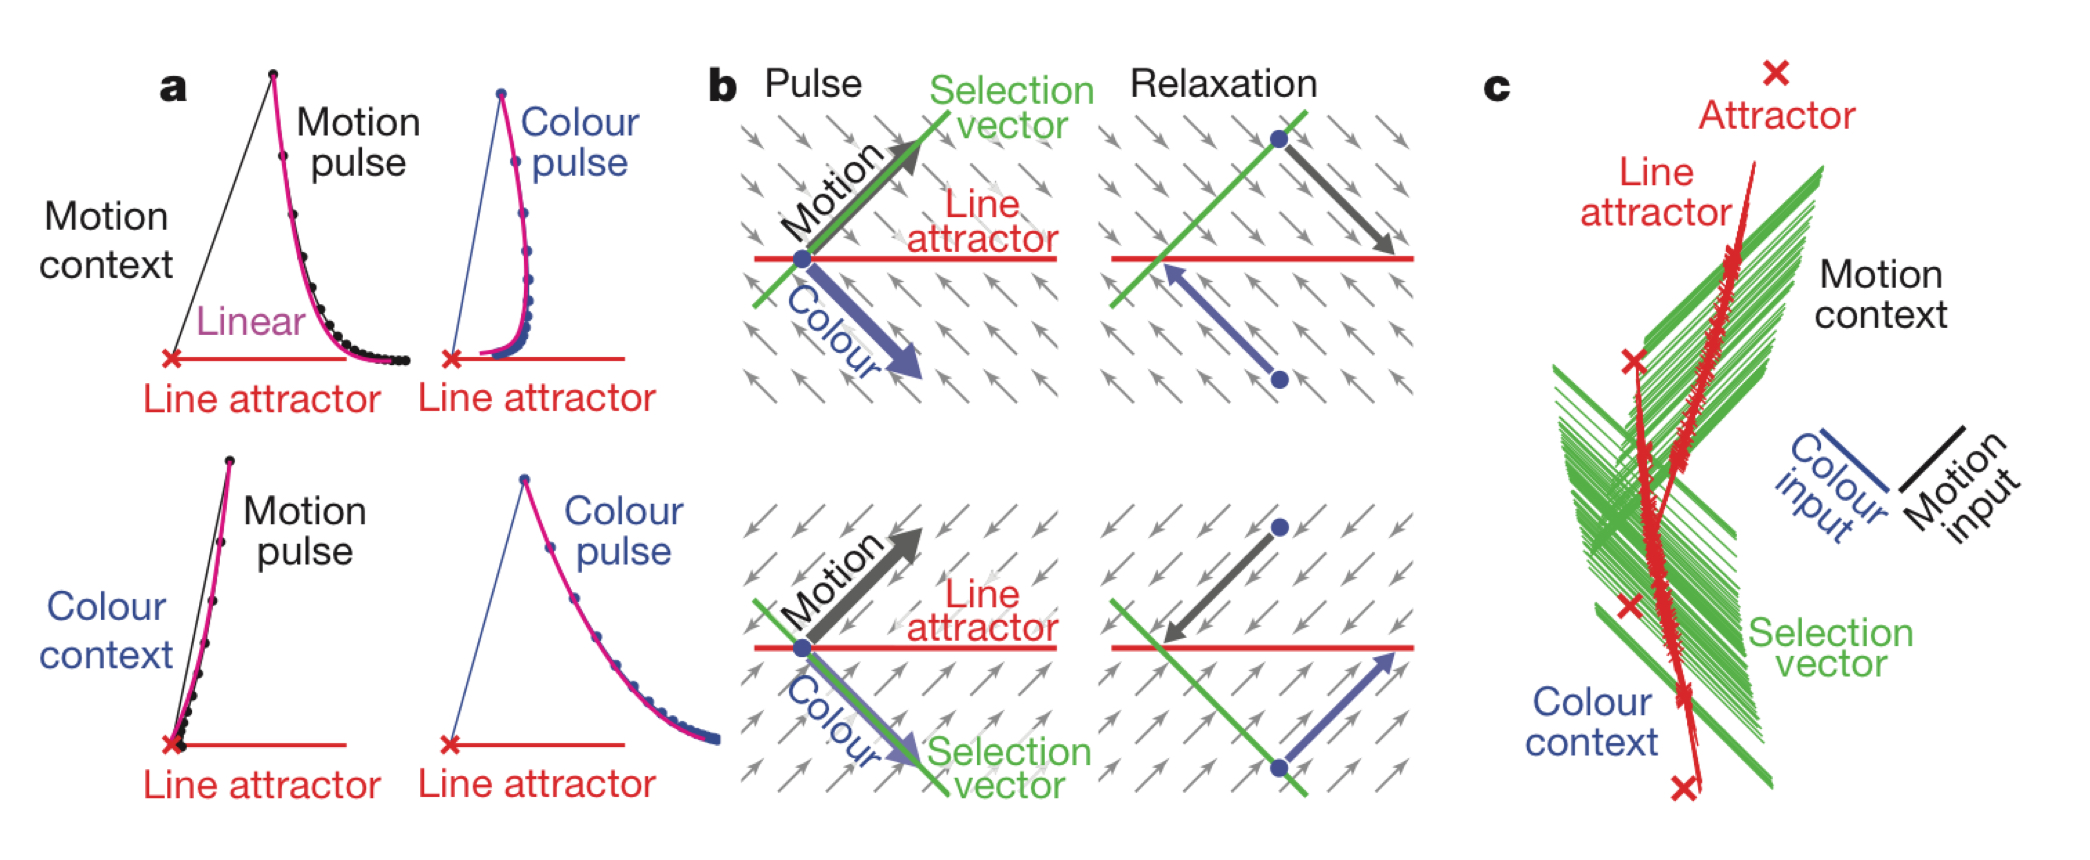
\includegraphics[width=0.8\textwidth]{./Figs/PFC7.jpeg}
    \caption{Interpretation of the dynamics - the context changes the landscape of the Line attractor. 
    The inputs directons are preserved, but the way the trajectories relax back to the line attractor is different.}
    \label{fig:PFC_NN_explained}
\end{figure}

\subsubsection{Assumptions/Criticisms/Questions}
\begin{enumerate}
    \item Are more areas other than PFC take part in the decision-making?
    \item How realistic is the trained network? For example, having two channels for inputs.
    \item If our artificial network found a solution, what can we say about the brain? How robust is the solution to different details/parameters?
    \item Are the RNN results influenced by the design of the network?
\end{enumerate}


%
%
%
%
%
%
%
%
%
%
%
%
%
%
%
%


\chapter{Reinforcement Learning}

\section{Pavlovian conditioning and the delta rule (Rescorla-Wagner)}

\subsection{Pavlovian Conditioning}

Pavlovian conditioning, also known as classical conditioning, was first described by Ivan Pavlov in 1904, earning him the Nobel Prize. 
The fundamental concept involves pairing a neutral stimulus, known as the conditioned stimulus (CS), with an unconditioned stimulus (US) that naturally triggers a response. 
Over time, the conditioned stimulus alone is able to evoke a similar response.
Before training, the US alone provokes an unconditioned response, while the CS does not. During training, the CS and US are presented together, leading to the conditioned response after training when the CS is presented alone.

\begin{figure}[ht]
\centering
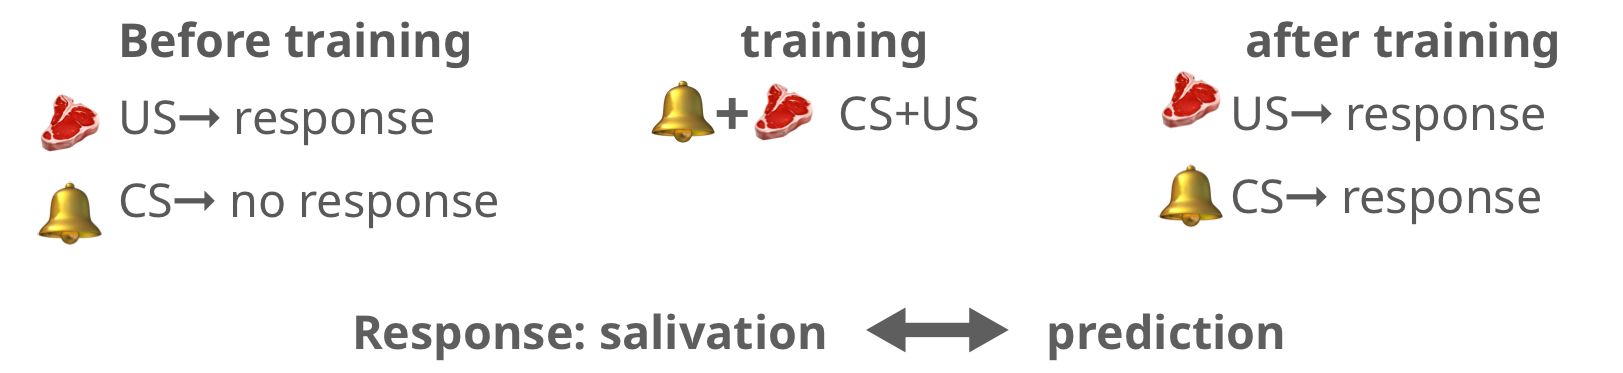
\includegraphics[width=\textwidth]{./Figs/pavlov.jpeg}
\caption{Pavlovian conditioning.}
\label{fig:pavlovian_conditioning}
\end{figure}

%
%
%

\subsection{The Rescorla-Wagner Model}
The Rescorla-Wagner model, introduced in 1972, provides a formal framework to predict the strength of learning and conditioning based on stimulus presentation. It is encapsulated by the delta rule, which is expressed mathematically as:
\begin{equation}
    \Delta w_i = \eta \delta s_i \quad \text{where} \quad \delta = u - r
\end{equation}
Here, 
\begin{itemize}
    \item \( r = \sum_i s_i w_i \) (response) represents the linear prediction of an unconditioned stimulus based on the conditioned stimuli
    \item \( w_i \) denotes the weight or strength of association of the \( i \)-th CS with the US
    \item u signifies the actual unconditioned stimulus 
    \item \( \delta \) signifies the prediction error 
    \item \( \eta \) is the learning rate. 
\end{itemize}

The key findings from experiments using this model include:
\begin{itemize}
    \item \textbf{Acquisition:} The strength of the CS-US association increases over conditioning trials.
    \item \textbf{Extinction:} If the CS is presented without the US in subsequent trials, the conditioned response gradually weakens.
    \item \textbf{Partial Reinforcement:} A CS presented with and without the US intermittently leads to a slower acquisition but a more resilient response.
    \item \textbf{Overshadowing:} If two CSs are presented together with the US, the stronger CS will acquire a greater association with the US.
    \item \textbf{Blocking:} If a CS is established as a predictor of the US, introducing a second CS does not lead to association with the US.
    \item \textbf{Inhibitory Conditioning:} A CS can be associated with the absence of a US, leading to a conditioned response of reduced probability.
    \item \textbf{Secondary Conditioning:} A CS associated with the US can in turn be used to condition another neutral stimulus. (The delta model falied to predict this phenomenon.)
\end{itemize}

These principles demonstrate that the Rescorla-Wagner model is a powerful tool for understanding basic learning processes, but it is not without limitations. 
The model does not fully account for more complex behaviors observed in associative learning, 
such as higher-order conditioning, where associations are built between stimuli without direct reinforcement. 
The linear framework of the Rescorla-Wagner model also struggles with complex, non-stationary environments where actions alter the state of the environment.

\begin{figure}[ht]
    \begin{subfigure}[b]{0.33\textwidth}
        \centering
        \includegraphics[width=\textwidth]{./Figs/acquisiton_exp.jpeg}
        \caption{Acquisition.}
        \label{fig:rescorla_wagner}
    \end{subfigure}
    \begin{subfigure}[b]{0.31\textwidth}
        \centering
        \includegraphics[width=\textwidth]{./Figs/extinction_exp.jpeg}
        \caption{Extinction.}
        \label{fig:overshadowing}
    \end{subfigure}
    \begin{subfigure}[b]{0.31\textwidth}
        \centering
        \includegraphics[width=\textwidth]{./Figs/partial_exp.jpeg}
        \caption{Partial reinforcement.}
        \label{fig:blocking}
    \end{subfigure}
    \begin{subfigure}[b]{0.5\textwidth}
        \centering
        \includegraphics[width=\textwidth]{./Figs/overshadow_exp.png}
        \caption{Overshadowing.}
        \label{fig:rescorla_wagner}
    \end{subfigure}
    \begin{subfigure}[b]{0.5\textwidth}
        \centering
        \includegraphics[width=\textwidth]{./Figs/blocking_exp.jpeg}
        \caption{blocking.}
        \label{fig:overshadowing}
    \end{subfigure}
    \begin{subfigure}[b]{0.5\textwidth}
        \centering
        \includegraphics[width=\textwidth]{./Figs/inhibitory_exp.jpeg}
        \caption{Inhibitory conditioning.}
        \label{fig:blocking}
    \end{subfigure}
    \begin{subfigure}[b]{0.5\textwidth}
        \centering
        \includegraphics[width=\textwidth]{./Figs/secondary_exp.jpeg}
        \caption{Secondary conditioning.}
        \label{fig:blocking}
    \end{subfigure}
    \label{fig:rescorla_wagner}
    \caption{Rescorla-Wagner model and associated phenomena.}
\end{figure}

%
%
%
%
%


\section{Definitions}

\begin{definition}[Markov decision process (MDP)]\ \\
    A Markov Decision Process (MDP) is a tuple $(S, A, P_{s,a}(\cdot) , R_s(\cdot), \gamma)$, where:
    \begin{itemize}
        \item $S$ is the state space.
        \item $A$ is the action space.
        \item $P_{s,a}(\cdot)$ is the transition probability function, $P_{s,a}(s') = \mathbb{P}(s_{t+1} = s' | s_t = s, a_t = a)$.
        \item $R_s(\cdot)$ is the reward function, $R_s(a) = \mathbb{E}[r_{t+1} | s_t = s, a_t = a]$.
        \item $\gamma$ is the discount factor.
    \end{itemize}    
    
\end{definition}

\begin {definition}[Policy]\ \\
    A policy $\pi$ is a mapping from state to probability distribution over actions, \\
    $\pi(s, a) = \mathbb{P}(a_t = a | s_t = s)$.

\end{definition}
The sum of all future rewards may theoretically be infinite, for a reasonable maximimization problem in such cases we can consider a fixed horizon $T$.

\begin {definition}[Expected return]\ \\
    The goal of an agent is to find a policy that maximizes the expected return -
    \begin{align*}
        &G_t = \sum_{k=0}^{\infty} \gamma^k r_{t+k+1} \quad &\text{where} \quad 0 \leq \gamma \leq 1 \\
        \text{or} \quad &G_t = \sum_{k=1}^{T-t}  r_{t+k} \quad &\text{where} \quad 0 \leq \gamma \leq 1
    \end{align*}
\end{definition}


\begin{definition}[Value function]\ \\
    The value function $V^{\pi}(s)$ is the expected return starting from state $s$ and following policy $\pi$.
    \begin{align*}
        v^{\pi}(s) = \mathbb{E}_{\pi} \left[ G_t | s_t = s \right]
    \end{align*}
\end{definition}


\begin{definition}[q function (value-action function)]\ \\
    The Q function $q^{\pi}(s, a)$ is the expected return starting from state $s$, taking action $a$, and following policy $\pi$.
    \begin{align*}
        q^{\pi}(s, a) = \mathbb{E}_{\pi} \left[ G_t | s_t = s, a_t = a \right]
    \end{align*}
\end{definition}


\subsection{Bellman equation}
\begin{definition}[Bellman equation]\ \\
    The Bellman equation for the value function is given by:
    \begin{align*}
        &v^{\pi}(s) = \mathbb{E}_{\pi} \left[ R_{t+1} + \gamma G_{t+1} | s_t = s \right] = \mathbb{E}_{\pi} \left[ R_{t+1} \right] + \gamma \mathbb{E} \left[ v^{\pi}(s_{t+1}) \right]  = \\
        &\sum_{a \in A} \pi(s, a) \left[ R_s(a) + \gamma \sum_{s' \in S} P_{s,a}(s') v^{\pi}(s') \right] = \\
        &\sum_{a \in A} \pi(s, a) q^{\pi}(s, a)
    \end{align*}
    The Bellman equation for the q function is given by:
    \begin{align*}
        q^{\pi}(s, a) = R_s(a) + \gamma \sum_{s' \in S} P_{s,a}(s') \sum_{a' \in A} \pi(s', a') q^{\pi}(s', a')
    \end{align*}
\end{definition}

\begin{figure}
    \begin{subfigure}[b]{0.5\textwidth}
        \centering
        \includegraphics[width=\textwidth]{./Figs/bellman-value.png}
        \caption{Value function.}
        \label{fig:mdp}
    \end{subfigure}
    \begin{subfigure}[b]{0.5\textwidth}
        \centering
        \includegraphics[width=\textwidth]{./Figs/bellman-q.png}
        \caption{Q function.}
        \label{fig:mdp_graph}
    \end{subfigure}
    \label{fig:mdp}
    \caption{Bellman equations}
\end{figure}

\begin{corollary}[Bellman equation (Matrix form)]\ \\
    The Bellman equation can be written in matrix form as:
    \begin{align*}
        \vec{v}^{\pi} = \vec{R}^{\pi} + \gamma \mathcal{T}^{\pi} \vec{v}^{\pi}
    \end{align*}
    where:
    \begin{itemize}
        \item $\vec{v}^{\pi}$ is the value function vector (entry $i$ is the value of state $i$ under policy $\pi$).
        \item $\vec{R}_s^{\pi} = \sum_{a \in A} \pi(s, a) R_s(a)$ is the expected reward vector for each state under policy $\pi$.
        \item $\mathcal{T}_{ss'}^{\pi} = \sum_{a \in A} \pi(s, a) P_{s,a}(s')$ is the transition probability matrix under policy $\pi$.
    \end{itemize}
    And the solution is given by:
    \begin{align*}
        \vec{v}^{\pi} = (I - \gamma \mathcal{T} ^{\pi})^{-1} \vec{R}^{\pi}
    \end{align*}

\end{corollary}


\subsection{Bellman optimality}
\begin{remark*}
    The value of a state depends on the policy, and induce a partial order over the policies: 
    \begin{align*}
        \pi \geq \pi' \quad \iff \quad v^{\pi}(s) \geq v^{\pi'}(s) \quad \forall s \in S
    \end{align*}
\end{remark*}

\begin{definition}[Optimal value function]\ \\
    The optimal value function $v^*(s)$ is the maximum expected return starting from state $s$.
    \begin{align*}
        v^*(s) = \max_{\pi} v^{\pi}(s) = \max_{\pi} q(s, \pi(s)) = \max_{a} \{R_s(a) + \gamma \sum_{s' \in S} P_{s,a}(s') v^*(s') \} \forall s \in S
    \end{align*}
\end{definition}

\begin{theorem}[Bellman optimality equation]\ \\
    \begin{enumerate}
        \item The optimal value function $v^*(s)$ satisfies the Bellman optimality equation, and is unique on condition that S, A are finite and $0 < \gamma < 1$.
        \item There exists an optimal policy $\pi^*$ s.t. $v^*(s) = v^{\pi^*}(s)$, i.e., $\pi^* \geq \pi \quad \forall \pi $. \\
        Moreover, $\pi^*$ is deterministic and is given by:
        \begin{align*}
            \pi^*(s) = \argmax_{a} \{R_s(a) + \gamma \sum_{s' \in S} P_{s,a}(s') v^{\pi^*}(s') \}
        \end{align*}
    \end{enumerate}
\end{theorem}

\section{Model-based methods}

\begin{definition}[Model-based RL]
    In model-based RL, we have a working model of the environment, and we use this model to plan ahead and make decisions.
    In the MDP framework, this means we know the transition probabilities $P_{s,a}(s')$ and the reward distribution $R_s(a)$.
\end{definition}

\begin{figure}
    \centering
    \includegraphics[width=0.5\textwidth]{./Figs/model_based_RL.jpeg}
    \caption{Model-based RL.}
    \label{fig:model_based}
\end{figure}

\subsection{Dynamic programming}

\begin{definition}[Dynamic programming]\ \\
    Dynamic programming is a method for solving complex problems by breaking them down into simpler subproblems. 
\end{definition}

For example, the shortest path problem can be solved using dynamic programming by breaking it down into subproblems of finding the shortest path from each node to the destination.

In the context of reinforcement learning, dynamic programming algorithms compute the value function by iteratively applying the Bellman optimality equation.

\subsection{Iterative policy evaluation}
\begin{algorithm}[H] 
    \SetAlgoLined
    \KwIn{MDP $(S, A, P_{s,a}(\cdot), R_s(\cdot), \gamma)$, policy $\pi$} 
    \KwOut{Value function $v^{\pi}(s)$}
    Initialize $v(s) \quad \forall s \in S$ \\
    \While{not converged}{
        \For{each state $s \in S$}{
            $v(s) \leftarrow \sum_{a \in A} \pi(s, a) \{R_s(a) + \gamma \sum_{s' \in S} P_{s,a}(s') v(s') \}$
        }
    }
    \caption{Iterative policy evaluation\label{Iterative policy evaluation}}
\end{algorithm}

%
%

\subsection{Policy iteration}
\begin{algorithm}[H] 
    \SetAlgoLined
    \KwIn{MDP $(S, A, P_{s,a}(\cdot), R_s(\cdot), \gamma)$}
    Initialize $\pi(s) \quad \forall s \in S$ \\
    \While{not converged}{
        \For{each state $s \in S$}{
            $\pi(s) \leftarrow \argmax_{a} \{R_s(a) + \gamma \sum_{s' \in S} P_{s,a}(s') v(s') \}$
        }
        Evaluate $v^{\pi}(s)$ using iterative policy evaluation.
    }
    \caption{Policy iteration\label{Policy iteration}}
\end{algorithm}

\begin{figure}
    \centering
    \includegraphics[width=0.9\textwidth]{./Figs/policy_iteration.png}
    \caption{Policy iteration.}
    \label{fig:policy_iteration}
\end{figure}

\begin{figure}
    \centering
    \includegraphics[width=0.5\textwidth]{./Figs/policy_iter.png}
    \caption{Policy iteration in a small Gridworld.}
    \label{fig:policy_iter}
\end{figure}
%
%

\subsection{Value iteration}

The idea behind value iteration is to iteratively update the value function until convergence, in contrast to policy iteration, 
which alternates between policy evaluation and policy improvement.

\begin{algorithm}[H] 
    \SetAlgoLined
    \KwIn{MDP $(S, A, P_{s,a}(\cdot), R_s(\cdot), \gamma)$} 
    \KwOut{Optimal value function $v^*(s)$}
    Initialize $v(s) \quad \forall s \in S$ \\
    \While{not converged}{
        \For{each state $s \in S$}{
            $v(s) \leftarrow \max_{a} \{R_s(a) + \gamma \sum_{s' \in S} P_{s,a}(s') v(s') \}$
        }
    }
    \caption{Value iteration\label{Value iteration}}
\end{algorithm}


%
%
%
%
%
%


\section{Model-free methods}

\begin{definition}[Model-free RL]
    In model-free RL, there is no explicit knowledge of the environment, and the agent learns by interacting with the environment.
    In the MDP framework, this means we do not know the transition probabilities $P_{s,a}(s')$ or the reward distribution $R_s(a)$.
    The goal is to learn a policy while interacting with the environment, using trial and error.
\end{definition}



\subsection{Value-based methods VS Policy-based methods}
\begin{definition}[Value-based methods]\ \\
    Value-based methods learn the optimal value function $v^*(s)$ or the optimal Q function $q^*(s, a)$ and derive the optimal policy from it.
\end{definition}

\begin{definition}[Policy-based methods]\ \\
    Policy-based methods learn the optimal policy directly without learning any value function.
\end{definition}


\subsection{Value-based Model-free methods}


\subsubsection{Monte Carlo}
The most straightforward model-free method is Monte Carlo (MC) learning, which estimates the value function by averaging the returns from multiple episodes.

\begin{algorithm}[H] 
    \SetAlgoLined
    \KwIn{MDP $(S, A, P_{s,a}(\cdot), R_s(\cdot), \gamma)$} 
    \KwOut{Value function $v^{\pi}(s)$}
    Initialize $v(s) \quad \forall s \in S$ \\
    \While{not converged}{
        Generate an episode $(s_1, r_1) \rightarrow (s_2, r_2) \ldots \rightarrow (s_n, r_n)$ using policy $\pi$ \\
        $R \leftarrow \sum_{k=1}^{n} \gamma^k r_{k}$ \\
        \For{each state $s_k$ in the episode}{
            $v(s_k) \leftarrow v(s_k) + \frac{1}{n} (R - v(s_k))$
        }
    }
    \caption{Monte Carlo prediction\label{Monte Carlo prediction}}
\end{algorithm}
After many episodes, this procedure guarantees convergence to the true value function, but it can be computationally expensive.

\subsubsection{Temporal difference learning (TD)}
Temporal difference (TD) learning is a model-free method that learns from incomplete epsiodes, by bootstrapping from the current estimate of the value function.
TD can learn before knowing the final outcome or without any final outcome, and it is more efficient than MC learning.

\begin{algorithm}[H]
    \SetAlgoLined
    \KwIn{MDP $(S, A, P_{s,a}(\cdot), R_s(\cdot), \gamma)$} 
    \KwOut{Value function $v^{\pi}(s)$}
    Initialize $v(s) \quad \forall s \in S$ \\
    \While{not converged}{
        Initialize state $s_0, \quad t=0$ \\
        \While{not terminal}{
            Take action $a$ using policy $\pi$ \\
            Observe reward $r_{t+1}$ and next state $s_{t+1}$ \\
            $v(s_t)\leftarrow v(s_t) + \alpha (r_{t+1} + \gamma v(s_{t+1}) - v(s))$ \\
            $t \leftarrow t+1$
        }
    }
    \caption{Temporal difference learning (TD(0))\label{Temporal difference learning}}
    
\end{algorithm}

\begin{figure}
    \centering
    \includegraphics[width=0.8\textwidth]{./Figs/MC_vs_TD.png}
    \caption{Monte Carlo vs Temporal Difference learning.}
    \label{fig:TD_learning}
\end{figure}

The differences between MC and TD learning are: 
\begin{itemize}
    \item Bias and variance:
        \begin{itemize}
            \item MC has high variance and zero bias.
            \item TD has low variance and some bias (it is more sensitive to initial values).
        \end{itemize}
    \item Learning process:
        \begin{itemize}
            \item MC must wait until the end of the episode to update the value function. 
            Can learn only from complete sequences of episodic environments.
            \item TD can learn before knowing the final outcome, and online after each step. 
            Can learn from complete or incomplete sequences of continuing or episodic environments.
        \end{itemize}
    \item Convergence:
        \begin{itemize}
            \item MC converges to solution with minimum mean squared error (usually more effective in non-Markov environments).
            \item TD(0) converges to solution of max likelihood Markov model (usually more effective in Markov environments).
        \end{itemize}
\end{itemize}

\begin{figure}
    \begin{subfigure}[b]{0.3\textwidth}
        \centering
        \includegraphics[width=\textwidth]{./Figs/MC_tree.png}
        \caption{Monte Carlo.}
        \label{fig:MC_tree}
    \end{subfigure}
    \begin{subfigure}[b]{0.3\textwidth}
        \centering
        \includegraphics[width=\textwidth]{./Figs/TD0_tree.png}
        \caption{Temporal Difference (0).}
        \label{fig:TD_tree}
    \end{subfigure}
    \begin{subfigure}[b]{0.3\textwidth}
        \centering
        \includegraphics[width=\textwidth]{./Figs/DP_tree.png}
        \caption{Dynamic Programming.}
        \label{fig:DP_tree}
    \end{subfigure}
    \label{fig:variance}
    \caption{Prediction methods comparison.}
\end{figure}


\subsubsection{The TD(n) error and learning rule}
The TD error is the difference between the predicted value and the target value, and it is used to update the value function.
We can genralize the expected return to more than observing one step ahead: 
\begin{align*}
    G_t^{(1)} &= r_{t+1} + \gamma v(s_{t+1}) &\quad \textbf{(TD(0))} \\
    G_t^{(2)} &= r_{t+1} + \gamma r_{t+2} + \gamma^2 v(s_{t+2}) \\
    \ldots \\
    G_t^{(\infty)} &= r_{t+1} + \gamma r_{t+2} + \ldots + \gamma^{T-1} r_{T} &\quad \textbf{(MC)}
\end{align*}
And in general, the n-step return is given by:

\begin{definition}[n-step return]\ \\
    \begin{align*}
        G_t^{(n)} &= r_{t+1} + \gamma r_{t+2} + \ldots + \gamma^{n-1} r_{t+n} + \gamma^n v(s_{t+n})
    \end{align*}
\end{definition}

\begin{definition}[TD(n) error]\ \\
    The TD(n) error is the difference between the n-step return and the current estimate of the value function.
    \begin{align*}
        \delta_t^{(n)} = G_t^{(n)} - v(s_t)
    \end{align*}
\end{definition}

\begin{algorithm}[H]
    \SetAlgoLined
    \KwIn{MDP $(S, A, P_{s,a}(\cdot), R_s(\cdot), \gamma)$} 
    \KwOut{Value function $v^{\pi}(s)$}
        The same as TD(0) but with update rule: 
        \begin{align*}
            v(s_t) &\leftarrow v(s_t) + \alpha \delta_t^{(n)} \\ 
            &= v(s_t) + \alpha (G_t^{(n)} - v(s_t)) \\ 
            &= v(s_t) + \alpha (r_{t+1} + \gamma r_{t+2} + \ldots + \gamma^{n-1} r_{t+n} + \gamma^n v(s_{t+n}) - v(s_t))
        \end{align*}
    \caption{Temporal difference learning (TD(n)) (Forword view) \label{Temporal difference learning}}
\end{algorithm}

\subsubsection{Backward view of TD and eligibility traces}
The forward view of $TD(n)$ (or $TD(\lambda)$) requires storing the n-step return for each state, which can be computationally expensive.
The backward view of $TD(n)$ uses eligibility traces to update the value function, which is more computationally efficient - 
in that way we can update the value function online for all states at once, from incomplete sequences of episodes.


\begin{figure}[ht]
    \centering
    \includegraphics[width=0.5\textwidth]{./Figs/RL_credit_assignment.png}
    \caption{Credit assignment problem in RL.}
    \label{fig:eligibility_traces}
\end{figure}

When we are discussing the $\textbf{Credit assignment problem}$ in RL, we don't know which state was responsible for the reward at each time step,
so we consider 2 heuristics:
\begin{itemize}
    \item $\textbf{Frequence heuristic}$: The more often a state is visited, the more credit it gets.
    \item $\textbf{Recency heuristic}$: The more recent a state is visited, the more credit it gets.
\end{itemize}

\begin{definition}[Eligibility traces]\ \\
    The eligibility trace $E_t(s)$ is a vector that keeps track of the eligibility of each state for updating the value function.
    \begin{align*}
        \vec{E}_0(s) &= 0 \\
        \vec{E}_t(s) &= \gamma \lambda \vec{E}_{t-1}(s) + \mathds{1}(s = s_t)
    \end{align*}
    where:
    \begin{itemize}
        \item $\gamma$ is the discount factor that determines the importance of future rewards (it is given by the problem definition).
        \item $\lambda$ is the eligibility trace decay parameter.
        \item $\mathds{1}(s = s_t)$ is the indicator function.
    \end{itemize}
\end{definition}

\begin{figure}
    \centering
    \includegraphics[width=0.7\textwidth]{./Figs/Backword_TD.png}
    \caption{Backward view of TD learning.}
    \label{fig:eligibility_traces}
\end{figure}

\begin{algorithm}[H]
    \SetNoFillComment
    \SetAlgoLined
    \KwIn{MDP $(S, A, P_{s,a}(\cdot), R_s(\cdot), \gamma)$, $\lambda \in [0, 1]$, $\alpha > 0$, $\pi$} 
    \KwOut{Value function $v^{\pi}(s)$}
    Initialize $v(s) \quad \forall s \in S$ and $\vec{E}_0(s) = 0 \quad \forall s \in S$ \\
    \While{not converged}{
        Initialize state $s_0, \quad t=0$ \\
        \While{not terminal}{
            Take action $a$ using policy $\pi$ \\
            Observe reward $r_{t+1}$ and next state $s_{t+1}$  \\ 
            $\delta_t = r_{t+1} + \gamma v(s_{t+1}) - v(s_t)$  \tcp*[l]{Compute TD error}
            $v(s) \leftarrow v(s) + \alpha \delta_t E_t(s)$ \tcp*[l]{Update val fun based on the error and eligibility}
            $t \leftarrow t+1$ \\
            $\vec{E}_t(s) \leftarrow \gamma \lambda \vec{E}_{t-1}(s) + \mathds{1}(s = s_t)$ \tcp*[l]{Update eligibility trace}
        }
    }
    \caption{Temporal difference learning with eligibility traces (TD($\lambda$))} \label{Temporal difference learning}
\end{algorithm}

When $\lambda = 0$, the eligibility trace is a one-step trace, and the algorithm is equivalent to TD(0).
When $\lambda = 1$, the eligibility trace is a complete trace, and the algorithm is equivalent to MC in case of offline update (after the end of the episode).

\medbreak
$\textbf{Issues with value-based TD algorithms}$ \\
\begin{itemize}
    \item With TD(n) we can learn the optimal value function without knowing the model of the environment.
    \item But when we want to extract the optimal policy from the value function, there is a problem: we need to know the model of the environment.
    \begin{align*}
        \pi^*(a|s) = \argmax_{a} \{R_s(a) + \gamma \sum_{s' \in S} P_{s,a}(s') v^*(s') \}
    \end{align*}
    So we still need a model to extract the optimal policy (we don't know the transition probabilities $P_{s,a}(s')$).
\end{itemize}


\subsubsection{On-policy VS Off-policy}
\begin{definition}[On-policy methods]\ \\
    On-policy methods learn the value function for the policy that is used to make decisions. \\
    Learn about policy $\pi$ from experience sampled from policy $\pi$.
\end{definition}
\begin{definition}[Off-policy methods]\ \\
    Off-policy methods learn the value function for a different policy than the one used to make decisions. \\
    Learn about policy $\pi$ from experience sampled from policy $\mu$.
\end{definition}


\subsubsection{SARSA algorithm}
The SARSA algorithm is an on-policy TD control algorithm that learns the Q function for the policy that is used to make decisions. \\
The name SARSA comes from the sequence of states, actions, rewards, states, and actions. 
The idea is to apply the TD update rule to the Q function, and then update the policy based on the new Q function while using $\epsilon$-greedy exploration.

\begin{algorithm}[H]
    \SetNoFillComment
    \SetAlgoLined
    \KwIn{MDP $(S, A, P_{s,a}(\cdot), R_s(\cdot), \gamma)$, $\epsilon > 0$, $\alpha > 0$} 
    \KwOut{Q function $q(s, a)$}
    Initialize $q(s, a) \quad \forall s \in S, a \in A$ \\
    \While{not converged}{
        Initialize state $s_0, \quad t=0$ \\
        Choose action $a_0$ using $\epsilon$-greedy policy based on $q$ \\
        \While{not terminal}{
            Take action $a_t$ \\
            Observe reward $r_{t+1}$ and next state $s_{t+1}$  \\ 
            Choose action $a_{t+1}$ using $\epsilon$-greedy policy based on $q$ \\
            $\delta_t = r_{t+1} + \gamma q(s_{t+1}, a_{t+1}) - q(s_t, a_t)$  \tcp*[l]{Compute TD error}
            $q(s_t, a_t) \leftarrow q(s_t, a_t) + \alpha \delta_t$ \tcp*[l]{Update Q function}
            $t \leftarrow t+1$ \\
        }
    }
    \caption{SARSA algorithm} \label{SARSA algorithm}
\end{algorithm}

\begin{figure}[ht]
    \begin{subfigure}[b]{0.5\textwidth}
        \centering
        \includegraphics[width=\textwidth]{./Figs/SARSA.png }
        \label{fig:SARSA}
    \end{subfigure}
    \begin{subfigure}[b]{0.5\textwidth}
        \centering
        \includegraphics[width=\textwidth]{./Figs/SARSA2.png}
        \label{fig:SARSA_tree}
    \end{subfigure}
    \label{fig:SARSA}
    \caption{SARSA algorithm.}
\end{figure}

\begin{figure}[ht]
    \centering
    \includegraphics[width=0.8\textwidth]{./Figs/SARSA_grid.png}
    \caption{SARSA($\lambda$) algorithm in a small Gridworld.}
    \label{fig:SARSA}
\end{figure}


\subsubsection{Q-learning algorithm}
The Q-learning algorithm is an off-policy TD control algorithm that learns the Q function for the optimal policy,
regardless of the policy that is used to make decisions. \\
Key ideas of Q-learning:
\begin{itemize}
    \item Next action is chosen using behavior policy $a_{t+1} \approx \mu(\cdot|s)$ (e.g., $\epsilon$-greedy).
    \item We consider alternative successor action $a' \approx  \pi(a| s_{t})$.
    \item We update the Q function towards the value of the alternative action.
    \item We allow both behavior and target policies to improve -
    \begin{itemize}
        \item The target policy $\pi$ is greeady with respect to the Q function.
        \begin{align*}
            \pi(a|s_{t+1}) = \argmax_{a} q(s_{t+1}, a)
        \end{align*}
        \item The behavior policy $\mu$ is $\epsilon$-greedy with respect to the Q function.
    \end{itemize}
    \item The Q-learning them simplifies:
    \begin{align*}
        q(s_t, a_t) \leftarrow q(s_t, a_t) + \alpha (r_{t+1} + \gamma \max_{a'} q(s_{t+1}, a') - q(s_t, a_t))
    \end{align*}
    \item The Q-learning control converges to the optimal action-value function $q^*(s, a)$.
\end{itemize}

\begin{algorithm}[H]
    \SetNoFillComment
    \SetAlgoLined
    \KwIn{MDP $(S, A, P_{s,a}(\cdot), R_s(\cdot), \gamma)$, $\epsilon > 0$, $\alpha > 0$} 
    \KwOut{Q function $q(s, a)$}
    Initialize $q(s, a) \quad \forall s \in S, a \in A$ \\
    \While{not converged}{
        Initialize state $s_0, \quad t=0$ \\
        \While{not terminal}{
            Choose action $a_t$ using $\epsilon$-greedy policy based on $q$ \\
            Take action $a_t$ \\
            Observe reward $r_{t+1}$ and next state $s_{t+1}$  \\ 
            $\delta_t = r_{t+1} + \gamma \max_{a'} q(s_{t+1}, a') - q(s_t, a_t)$  \tcp*[l]{Compute TD error}
            $q(s_t, a_t) \leftarrow q(s_t, a_t) + \alpha \delta_t$ \tcp*[l]{Update Q function}
            $t \leftarrow t+1$ \\
        }
    }
    \caption{Q-learning algorithm} \label{Q-learning algorithm}
\end{algorithm}

\begin{figure}
    \centering
    \includegraphics[width=0.8\textwidth]{./Figs/Q_Learning.png}
    \caption{Q-learning algorithm.}
    \label{fig:Q_learning}
\end{figure}



\subsubsection{Stochatic policies}
Why would we need stochastic policies?
\begin{itemize}
    \item in MDP, there is always an optimal deterministic policy.
    \item However, modt problems are not fully observable, and the optimal policy may be stochastic.
    \item Search space is smoother for stochastic policies $\rightarrow$ we can use gradient-based optimization.
    \item Exploration: Stochastic policies allow the agent to explore the environment and learn more about it.
\end{itemize}

\begin{definition}[The exploration vs exploitation dilemma]\ \\
    The exploration vs exploitation dilemma is the trade-off between exploring the environment to learn more about it and exploiting the current knowledge to maximize rewards.
\end{definition}

some exploration strategies:
\begin{itemize}
    \item $\textbf{Epsilon-greedy}$: With probability $\epsilon$ choose a random action, otherwise choose the greedy action.
    \begin{align*}
        \pi(a|s) = \begin{cases}
            1 - \epsilon + \frac{\epsilon}{|A|} & \text{if } a = \argmax_{a} q(s, a) \\
            \frac{\epsilon}{|A|} & \text{otherwise}
        \end{cases}
    \end{align*}

    \item $\textbf{Softmax}$: Choose actions according to the Boltzmann policy.
    \begin{align*}
        \pi(a|s) = \frac{e^{\beta q(s, a)}}{\sum_{a'} e^{\beta q(s, a')}}
    \end{align*}
\end{itemize}
Where we would decrease $\epsilon$ or increase $\beta$ over time to decrease exploration and increase exploitation.

\begin{figure}[ht]
    \centering
    \includegraphics[width=0.4\textwidth]{./Figs/softmax_example.jpeg}
    \caption{Softmax mapping example.}
    \label{fig:softmax}
\end{figure}

\begin{figure}[ht]
    \begin{subfigure}[b]{0.48\textwidth}
        \centering
        \includegraphics[width=\textwidth]{./Figs/epsilon_greedy_q2.jpeg}
        \label{fig:epsilon_greedy}
        \caption{Distance from the optimal policy}
    \end{subfigure}
    \begin{subfigure}[b]{0.5\textwidth}
        \centering
        \includegraphics[width=\textwidth]{./Figs/epsilon_greedy_q.jpeg}
        \caption{Average reward per episode}
        \label{fig:softmax}
    \end{subfigure}
    \label{fig:exploration}
    \caption{$epsilon$-greedy policy for q-learning on a gridworld.}  
\end{figure}


%
%
%


\subsection{Policy-based Model-free methods}
We have seen that the optimal policy can be found using the action-state value function
\begin{align*}
    \pi^*(a|s) = \argmax_{a} q^{*}(s, a)
\end{align*}
Instead, we can define a policy that optimizes an arbitrary parameterized function 
\begin{align*}
    \pi_\theta(a|s) = \argmax_{a} H(s, a |\theta)
\end{align*}
where $\theta$ are the parameters of the policy,
and the optimal policy is learned by adjusting the parameters $\theta$ to maximize the expected return.

We can also define a stochastic policy, e.g., Softmax / Boltzmann policy:
\begin{definition}[Softmax policy (Boltzmann policy)]\ \\
    \begin{align*}
        \pi(a|s) = \frac{e^{\beta H(s, a |\theta)}}{\sum_{a'} e^{\beta H(s, a' |\theta)}}
    \end{align*} 
\end{definition}





\subsubsection{Policy Gradient}
A simple policy based method scheme:
\begin{enumerate}
    \item Run many trials with different perturbated parameter sets $\theta^{(1)}, \theta^{(2)}, \ldots, \theta^{(N)}$.
    \item Fit a function of the parameters to the return value: $J(\theta) = \mathbb{E}[G]$.
    \item Update the parameters $\theta$ using the gradient of the function: $\theta \leftarrow \theta + \alpha \nabla_{\theta} J(\theta)$.
\end{enumerate}

\begin{theorem}[Policy Gradient Theorem]\ \\
    For any differentiable policy $\pi_{\theta}(a|s)$, let $d_0$ be the initial state distribution over states at the beginning of an episode.
    The policy gradient of $J(\theta) = \mathbb{E}_{\pi_{\theta}}[G | {s} \sim  d_0 ]$ is given by:
    \begin{align*}
        \nabla_{\theta} J(\theta) = 
            \mathbb{E}_{\pi_{\theta}} \left[ \sum_{t=0}^T \gamma^t \quad q_{\pi_{\theta}}(s, a) \quad \nabla_{\theta} \pi_{\theta}(a|s) 
            \quad | \quad \{s\} \sim  d_0 \right]
    \end{align*}    
\end{theorem}

\subsubsection{Score function (likelihood ratio)}
Likelihood ratios exploits the following identity:
\begin{align*}
    \nabla_{\theta} \pi_{\theta}(a|s) = \pi_{\theta}(a|s)\frac{\nabla_{\theta} \pi_{\theta}(a|s)}{\pi_{\theta}(a|s)} = \pi_{\theta}(a|s) \nabla_{\theta} \log \pi_{\theta}(a|s)
\end{align*}

\begin{definition}[The score function]\ \\
    The score function is the gradient of the log-likelihood of the policy:
    \begin{align*}
        \nabla_{\theta} \log \pi_{\theta}(a|s)
    \end{align*}
\end{definition}


\subsubsection{REINFORCE (Monte Carlo policy gradient)}
The REINFORCE algorithm is a policy gradient method that uses the score function to update the policy parameters.
We will use softmax policy as an examplem, and actions using linear combination of features: $\pi_\theta(a|s) = H(s, a |\theta) = \theta^T \phi(s, a)$. \\
Then the probability of taking action $a$ in state $s$ is given by:
\begin{align*}
    \pi_{\theta}(a|s) = \frac{e^{\theta^T \phi(s, a)}}{\sum_{a'} e^{\theta^T \phi(s, a')}}
\end{align*}
And the score function is given by:
\begin{align*}
    \nabla_{\theta} \log \pi_{\theta}(a|s) = \phi(s, a) - \mathbb{E}_{a \sim \pi_{\theta}}[\phi(s, a)]
\end{align*}

\begin{proof}
    \begin{align*}
        \nabla_{\theta} \log \pi_{\theta}(a|s) &= \nabla_{\theta} \log \left( \frac{e^{\theta^T \phi(s, a)}}{\sum_{a'} e^{\theta^T \phi(s, a')}} \right) \\
        &= \nabla_{\theta} \left( \theta^T \phi(s, a) - \log \sum_{a'} e^{\theta^T \phi(s, a')} \right) \\
        &= \phi(s, a) - \nabla_{\theta} \log \sum_{a'} e^{\theta^T \phi(s, a')} \\
        &= \phi(s, a) - \frac{\nabla \sum_{a'} e^{\theta^T \phi(s, a')}}{\sum_{a'} e^{\theta^T \phi(s, a')}} \\
        &= \phi(s, a) - \frac{\sum_{a'} \phi(s, a') e^{\theta^T \phi(s, a')}}{\sum_{a'} e^{\theta^T \phi(s, a')}} \\
        &= \phi(s, a) - \sum_{a'} \pi_{\theta}(a'|s) \phi(s, a') \\
        &= \phi(s, a) - \mathbb{E}_{a \sim \pi_{\theta}}[\phi(s, a)]
    \end{align*}
\end{proof}

Consider a simple class of one-step MDPs: 
\begin{align*}
    &J(\theta) = \mathbb{E}_{\pi_{\theta}}[G] = \sum_{s \in S} d_0(s) \sum_{a \in A} \pi_{\theta}(a|s) R_s(a) \\ 
    \nabla_{\theta} J(\theta) &= \sum_{s \in S} d_0(s) \sum_{a \in A} \pi_{\theta}(a|s) \nabla_{\theta} \log \pi_{\theta}(a|s) R_s(a) \\
    &= \mathbb{E}_{\pi_{\theta}} \left[ \nabla_{\theta} \log \pi_{\theta}(a|s) R_s(a) \right]
\end{align*}

\begin{theorem}[Policy Gradient Theorem (2)]\ \\
    For any differentiable policy $\pi_{\theta}(a|s)$, for any policy objective funcion $J(\theta)$, the policy gradient is given by:
    \begin{align*}
        \nabla_{\theta} J(\theta) = \mathbb{E}_{\pi_{\theta}} \left[ \nabla_{\theta} \log \pi_{\theta}(a|s) Q^{\pi_\theta}(s, a) \right]
    \end{align*}
    
\end{theorem}

\begin{algorithm}[H]
    \SetNoFillComment
    \SetAlgoLined
    \KwIn{MDP $(S, A, P_{s,a}(\cdot), R_s(\cdot), \gamma)$, $\alpha > 0$} 
    \KwOut{Policy parameters $\theta$}
    Initialize $\theta$ \\
    \While{not converged}{
        Generate an episode $(s_1, a_1, r_1) \rightarrow (s_2, a_2, r_2) \ldots \rightarrow (s_n, a_n, r_n)$ using policy $\pi_{\theta}$ \\
        \For{each step $t$ in the episode}{
            $G \leftarrow \sum_{k=t}^{n} \gamma^{k-t} r_{k}$ \\
            $\theta \leftarrow \theta + \alpha \nabla_{\theta} \log \pi_{\theta}(a_t|s_t) G$
        }
    }
    \caption{REINFORCE algorithm} \label{REINFORCE algorithm}
\end{algorithm}

\subsubsection{REINFORCE for neural networks}
\begin{figure}[ht]
    \centering
    \includegraphics[width=0.3\textwidth]{./Figs/single_neuron_reinforce.jpeg}
    \caption{Single neuron REINFORCE.}
    \label{fig:REINFORCE_NN}
\end{figure}

The setup: 
\begin{itemize}
    \item The activity of each neuron is given by a probability function $P(y_i = y | \vec{w}, \vec{x}) = g(y, \vec{w}, \vec{x})$. 
        \begin{itemize}
            \item Linear-nonlinear transformation: $P(y_i = y | \vec{w}^T \vec{x}) = g(y, \vec{w}^T\vec{x})$ where $g$ is a non linear function.
            \item Bernoulli neurons: $P(y_i = 1 | \vec{w}^T \vec{x}) =  \text{sign}(\vec{w}^T \vec{x})$.
            \item Logistic neurons: $P(y_i = 1 | \vec{w}, \vec{x}) = \frac{1}{1 + e^{-\vec{w}^T \vec{x}}}$.
        \end{itemize}
    \item At each step of the learning process:
    \begin{itemize}
        \item The environment provides input $\vec{x}^t \sim P_{input}(\vec{x})$.
        \item The system finds an output $\vec{y}^t$ that is understood as an action.
        \item The environment provides a reward $r^t \sim P(r | \vec{x}^t, \vec{y}^t)$ (a scalar value).
        \item Every neuron in the network receives the reward signal $r^t$ and updates its weights.
    \end{itemize}
    \item The goal of the network is to maximize the expected reward: $\langle r \rangle = R(W)$.
    \item We are averaging over few things:
    \begin{itemize}
        \item The input distribution $\vec{x}^t \sim P_{input}(\vec{x})$.
        \item The output distribution $\vec{y} \sim P(\vec{y} | \vec{x}, \vec{w}, g)$.
        \item The reward distribution $r^t \sim P(r | \vec{x}^t, \vec{y}^t)$.
    \end{itemize}
\end{itemize}

\begin{algorithm}[H]
    \SetNoFillComment
    \SetAlgoLined
    Initialize $\theta$ \\
    For each episode $t$ \\
    \begin{align*}
        \bigtriangleup W_{ij} = \alpha_{ij}(r - b_{ij})e_{ij} = \alpha_{ij}(r - b_{ij})\frac{\partial \ln  g_i}{\partial W_{ij}}
    \end{align*}
    where:
    \begin{itemize}
        \item $r$ is the reward signal.
        \item $b_{ij}$ is the baseline (reward threshold).
        \item $e_{ij}$ is the eligibility trace. The responsibility of a particular connection with respect to the output.
        \item $\alpha_{ij}$ is the learning rate (can be different for each synapse).
    \end{itemize}
    \caption{REINFORCE algorithm (of a NN)} \label{REINFORCE algorithm}
\end{algorithm}

\medbreak

Example: binary neuron with logistic activation function:
\begin{align*}
    P(y_i = 1 | \vec{w}, \vec{x}) = \frac{1}{1 + e^{-\vec{w}^T \vec{x}}}
\end{align*}
The eligibility trace is given by (here we take the derivative without log to simplify the expression):
\begin{figure}[ht]
    \centering
    \includegraphics[width=0.6\textwidth]{./Figs/sigmoid_function_derivative.png}
    \caption{Logistic neuron.}
    \label{fig:logistic_neuron}
\end{figure}

\begin{align*}
    e_{ij} = \frac{\partial P(y_i = 1 | \vec{w}, \vec{x})}{\partial w_{ij}} = P_i (1 - P_i) x_j
\end{align*}

\subsubsection{The analysis of the REINFORCE algorithm}
\textcolor{red}{TODO - stuff from homework assignment}

%
%
%
%
%
%
%
%
%
%
%
%
%
%
%
%

\chapter{Things that were not covered}

\section{Convergence of the perceptron learning algorithm}

\section{Uniqueness of the SVM solution (Vapnik, 1998)}

\section{Upper bound on the generalization error of the SVM}

\backmatter
% Add any appendices or references here

\end{document}







        

